\chapter{Kinematic weighting}
\label{chap:cpv:kinematic_weighting}

For the assumptions in \cref{eqn:cpv:theory:dacp} to hold, the
kinematics of the particles contributing to the background asymmetries must be 
equal between the \pKK\ and \ppipi\ final states.
These are the kinematics of the \PLambdab, the muon from the \PLambdab, and the 
proton from the \PLambdac.
Within a particular \phh\ final state, it must also be the case that the \Php\ 
and \Phm\ kinematics are equal for $\ADf(f)$ to only contain contributions from 
the proton detection asymmetry $\AD(\Pproton)$.
A comparison of these distributions between the 2012 magnet down \pKK\ and 
\ppipi\ datasets is given in 
\cref{fig:cpv:kinematic_weighting:pre:Lb,fig:cpv:kinematic_weighting:pre:Lb_mu,fig:cpv:kinematic_weighting:pre:Lc,fig:cpv:kinematic_weighting:pre:Lc_p,fig:cpv:kinematic_weighting:pre:pKK_h1h2,fig:cpv:kinematic_weighting:pre:ppipi_h1h2}.
The signal distributions are shown, where the contents of each bin is defined 
as the sum of signal sWeights within that bin, as computed from the result of 
the mass fit to the charge-combined samples described in 
\cref{chap:cpv:prelim_fits}.
The correlation of the variables with the \PLambdac\ mass is seen to be small, 
with a correlation coefficient less than \SI{2}{\percent} for all variables.
Only the muon kinematics across the modes and the \hmhp\ kinematics within the 
modes agree, and so a weighting is necessary.

A \acf{BDT} is used to equalise the relevant particle kinematics between the 
two modes.
This is an uncommon technique in physics analyses, with ratios of 
multi-dimensional histograms being used more often, and so it will be briefly 
summarised in the following, preceded by a introduction to decision trees in 
order to established the required terminology.
The creation of the specific models using for weighting will then be presented, 
followed by a discussion on weighting validation.

\section{Decision trees}
\label{chap:cpv:kinematic_weighting:bdt_theory}

Decision trees~\cite{breiman1984classification,Louppe:14077502} are one 
algorithm in the set of \acl{MVA} tools that also includes \acl{kNN} and 
\aclp{ANN}.
In \acl{HEP}, such tools are commonly used for the task of 
\emph{classification}, where one wishes to discriminate between several species 
that are mixed together, usually in unknown proportions, in the data.
Most generally, the algorithms try to estimate some function whose parameters 
are a set of variables $\vec{x}$, or \emph{features}, and when used for binary 
classification the function is the decision boundary, either side of which is a 
pure sample of each of the two species.
In practice, the generating \acp{PDF} for the species overlap to some degree, 
or the algorithm cannot distinguish them with certainty across the entire 
feature space.
For a given set of values of the features, the algorithm then returns a 
probability that the point $\vec{x}$ belongs to a particular species.
Throughout this \lcnamecref{chap:cpv:kinematic_weighting:bdt_theory}, only the 
problem of binary classification will be considered.

The rectangular cuts used in the selection described in 
\cref{chap:cpv:selection} are a crude attempt at a estimating the 
multidimensional decision boundary that separates signal from background, with 
the decision being either zero if at least one cut is not passed, or one if all 
cuts are passed.
A decision tree refines this approach by defining cuts which are conditional on 
the outcome of those preceding it.
This begins with a single \emph{node}, the \emph{root}, which defines a cut on 
a single feature $x$, say $x > y$ for some value $y$, by which the input sample 
is split in two.
The sample passing the cut is passed a node in the next \emph{layer}, whilst 
the failing sample is passed to another node in that layer.
Each of these nodes defines some other cut, possibly on a different feature, 
and the samples are further split and passed to nodes in the next layer.
Each of the $N$ layers can have up to $2^{n - 1}$ nodes, where $n$ is the 
\emph{depth} or layer number.
Eventually the sub-samples can proceed no further and reside in a \emph{leaf}, 
or terminal, node at which point a per-species probability is assigned to them.
An example decision tree is illustrated in 
\cref{fig:cpv:kinematic_weighting:decision_tree}.

\begin{figure}
  \centering
  % Adapted from http://www.texample.net/tikz/examples/decision-tree/
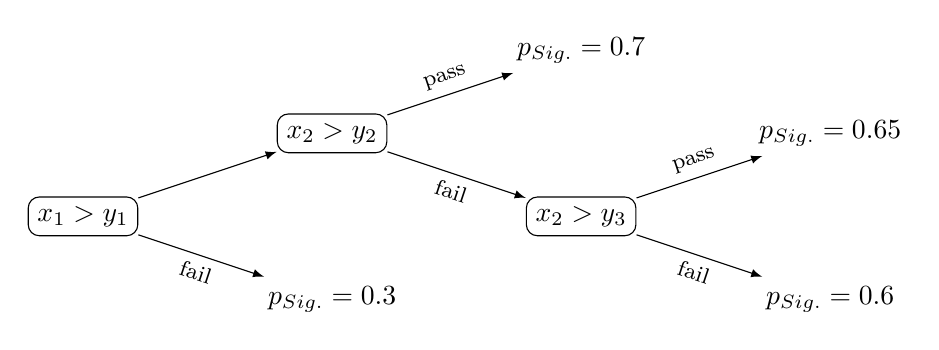
\begin{tikzpicture}
  [
    grow                    = right,
    sibling distance        = 6em,
    level distance          = 9em,
    edge from parent/.style = {draw, -latex,font=\footnotesize},
    sloped,
    treenode/.style = {shape=rectangle, rounded corners,
      draw, align=center},
    root/.style     = {treenode},
    env/.style      = {treenode},
    leaf/.style      = {treenode, draw=white}
  ]
  \node [root] {$x_{1} > y_{1}$}
    child { node [leaf] {$p_{\text{Sig.}} = 0.3$}
      edge from parent node [below] {fail} }
    child { node [env] {$x_{2} > y_{2}$}
      child { node [env] {$x_{2} > y_{3}$}
        child { node [leaf] {$p_{\text{Sig.}} = 0.6$}
          edge from parent node [below] {fail} }
        child { node [leaf] {$p_{\text{Sig.}} = 0.65$}
          edge from parent node [above] {pass} }
        edge from parent node [below] {fail} }
      child { node [leaf] {$p_{\text{Sig.}} = 0.7$}
        edge from parent node [above, align=center]
        {pass} }
    };
\end{tikzpicture}

  \caption{%
    A decision tree, computing signal probabilities $p_{\text{Sig.}}$ in the 
    leaf nodes using a set of features $x_{i}$ and cut values on those features 
    $y_{i}$.
  }
  \label{fig:cpv:kinematic_weighting:decision_tree}
\end{figure}

The construction, or growth, of a single decision tree is the process to 
determine which features and cut values are used in what nodes, and what the 
assigned probabilities should be in the terminal nodes.
There are many parameters available for tuning during construction, including: 
the maximum depth; the figure of merit the cut at each node should optimise; 
and the stopping criteria that determines whether additional nodes can be 
created.
Both tuning of these \emph{hyper-parameters} and of the features and cuts to 
use is a complex optimisation problem~\cite{Louppe:14077502}, the details of 
which are not necessary for understanding the classification problem at hand.
The important feature of the construction is that it is performed using an 
ensemble of individual \emph{events}, feature vectors $\vec{x}$, called the 
\emph{training} sample, in which the true species of each event is known.
This is typically a combination of some simulated \ac{MC} sample, known to be 
signal is known through truth-matching, and some sample from a control region 
in the data which is known to contain no signal, such as mass sidebands.
The decision tree then tries to fit the set of cuts and values such that the 
samples can be classified as cleanly as possible, given the hyper-parameters.
The probability of the terminal nodes can then be taken as, for example, the 
ratio of the two species that remain after the training sample has been passed 
through the final tree.

The discriminating power of a decision tree is driven by two factors: how 
discriminatory the set of features is between the two species; and what the 
values of the hyper-parameters are.
The exact choice of these is dependent on the nature of the classification 
problem, however the hyper-parameters should be chosen such that the decision 
tree is not \emph{over-fitted} to the training data.
This occurs when the tree is too sensitive to the statistical fluctuations in 
the features in the training sample.
It is possible that a tree with infinitely many layers would be able to 
perfectly classify the training sample, for example, but a new signal sample 
not present in the training may be classified as background, as the values of 
the features do not exactly match those in the training sample.
In general, over-fitting results in the performance of the tree being worse on 
an independent \emph{testing} sample, within which the true species are also 
known, than on the training sample.
When tuning the set of hyper-parameters, the performance of the tree should 
then be evaluated on the testing sample.
This is comparable with the normal fitting of functions to data with maximum 
likelihood or \chisq\ methods, in that more complex models can describe the 
data well, to an arbitrary degree for higher complexities, but the models begin 
to offer less general insight, instead being tailored to a specific dataset 
that happens to have been observed.
Measures of performance include the \emph{accuracy}, the number of correctly 
classified events relative to the total number, and the \emph{error rate}, the 
number of wrong predictions relative to the total number.
In the worst case, a classifier does no better at guessing event species than 
uniform random guessing.

The benefit of using decision trees over some other \ac{MVA} algorithms is that 
they can be intuitively interpreted: the tree can be visualised as such, and 
the decisions can be reasoned with by seeing how different features influence 
the lower depths of the tree.
However, a tree that fits the training sample well is in general very deep, as 
only one feature enters the decision in each node.
Deep trees are particularly susceptible to over-fitting, and so \emph{ensemble} 
methods are often used.

\subsection{Ensembles of trees and boosting}
\label{chap:cpv:kinematic_weighting:bdt_theory:ensembles}

The error rate of a decision tree, the fraction of incorrectly classified 
events, is due to two properties of the classifier: the bias, the consistent 
deviation away from the true values, and the variance, the spread around the 
mean value~\cite{Breiman96biasvariance}.
A complex model, prone to over-fitting, may have a low bias but a high 
variance, whereas a simple model may have a high bias but a low variance.

To reduce the variance of a tree-based classifier, ensembles of complex trees 
can be created, where each tree is grown using a subset of the training 
data~\cite{Breiman1996}.
The classification for an event is then determined using the set of 
classifications produced by the ensemble, such as by taking the mean of that 
set.
This does not increase the bias of the model if the predictions of the 
individual trees are uncorrelated.
To guard against this possibility, the technique of \emph{random 
  forests}~\cite{Breiman2001,Louppe:14077502} can be used, in which each node 
splitting can only use information from a random subset of the features, in 
addition to the random sub-sampling of the training data used to grow each tree 
in the ensemble.

The bias can be decreased by employing \emph{boosting}, for which 
\adaboost~\cite{Freund1997119} is commonly used algorithm.
Rather than training an ensemble of complex models in parallel, \adaboost\ 
trains a \emph{sequence} of \emph{weak learners} (decisions trees here), whose 
predictions are only slightly better than random guessing, and returns a 
weighted sum of their predictions as the final classification.
This begins by growing a single, shallow tree where the $i$th vector in the 
training sample is weighted with a weight $w_{i} = 1/N$.
The training sample is fed through the tree, and events which were classified 
incorrectly are assigned a larger weight, and those which were classified 
correctly are assigned a smaller weight.
A new tree is grown using the new weights, and the procedure is iterated.
With each iteration, events that are consistently incorrectly classified are 
given a greater importance in the training.

The generalisation of the \adaboost\ algorithm is \emph{gradient 
  boosting}~\cite{friedman2001}.
With \adaboost, additional weak learners compensate for previous incorrect 
classifications by being trained with specially weighted data.
In gradient boosting, additional weak learners try to correct the 
classification of the previous learners by fitting a regression model 
$f(\vec{x})$ to the residuals ${(\hat{y}_{i} - f(\vec{x}_{i}))}^2$ of the 
predicted classification $f(\vec{x}_{i}) = y_{i}$ and the true classification 
$\hat{y}_{i}$.
In this way, gradient boosting tries to minimise the \emph{loss function} that 
characterises how poorly the classifier is performing, and can be generalised 
by considering an arbitrary loss function $L(\hat{y}, f(x))$, which can be the 
residual.

\section{Weighting with decision trees}
\label{chap:cpv:kinematic_weighting:bdt_method}

It is common in \acl{HEP} to want to be able to bring two distributions into 
agreement, as is the case in this analysis where particle kinematics should be 
equal between the \pKK\ and \ppipi\ data.
Call one possibly multi-dimensional distribution the \emph{target} $f_{t}$ and 
the other the \emph{original} distribution $f_{o}$.
To transform $f_{o}$ to have the same form as $f_{t}$, there is some 
transformation function $W$
\begin{equation}
  f_{t}(x) = W(x)f_{o}(x),
\end{equation}
where $x$ is a possibly multi-dimensional parameter.
As the true distributions of $f_{t}$ and $f_{o}$ are not known in the data, 
they are approximated as histograms, partitioning the data in $x$ and counting 
the number of events that fall in each bin.
The transformation function is quantised as $w$ in bins, where in the $i$th bin
\begin{equation}
  f_{t}(x_{i}) = w(x_{i})f_{o}(x_{i}),
\end{equation}
and where $f_{t(o)}(x_{i})$ is the count of the target (original) distribution 
in the $i$th bin.
The histogram of $f_{o}$ can be transformed to that of $f_{t}$ by computing the 
per-bin \emph{weights}
\begin{equation}
  w(x_{i}) = \frac{f_{t}(x_{i})}{f_{o}(x_{i})}.
\end{equation}
This is valid assuming there are no bins where $f_{o}(x_{i}) = 0$.

To model the true \aclp{PDF} in $x$ as closely as possible, the histogram must 
have a fine enough binning that all structures are resolved.
Specifically, as in the determination of the \ac{PID} efficiency in 
\cref{chap:prod:effs:pid}, the binning must be fine enough such that difference 
between the true \acp{PDF} of the two distribution within any given bin are 
small.
This must be balanced with the limited statistical precision available in each 
bin: too fine a binning will result in the original distribution being weighted 
to match the statistical fluctuations in the target, rather than the physical 
features.
Limited sample sizes become particularly problematic for higher-dimensional 
weighting, when even 10 equally spaced bins per dimension in a 
three-dimensional binning requires $1,000$ bins.
Given physical distributions such as momentum and pseudorapidity, which have 
long tails, it can be difficult to invent a binning that avoids sparsely 
populated or empty bins whilst still accounting for differences in the 
distributions.

To overcome the limitations of histogram-based weighting, this analysis defers 
the computation of the per-event weights $w_{i}$ to a decision tree with 
gradient boosting~\cite{Rogozhnikov:2016bdp}.
The classifier is trained as in the gradient boosting method described in 
\cref{chap:cpv:kinematic_weighting:bdt_theory}, with the loss function
\begin{equation}
  L = \sum_{l \in \text{Leaves}} \frac{%
    {(w_{l,o} - w_{l,t})}^{2}
  }{%
    w_{l,o} + w_{l,t}
  },
\end{equation}
where $w_{l,t(o)}$ is the sum of target (original) weights in the $l$th leaf 
node of the regression tree.
For the initial iteration, and an unweighted set of training events, this is 
equal to the number of target (original) events in the leaf node.
This metric has the tree split the samples into regions where the differences 
between the sample sizes is maximal, and is chosen because these are the 
regions with the largest differences, and so the classifier should focus on 
weighting them.
Predictions $p_{l}$ within a leaf are computed as
\begin{equation}
  p_{l} = \log{\frac{w_{l,t}}{w_{l,o}}}.
\end{equation}
At the end of the $i$th iteration, each event from the `original' sample is 
weighted by $w_{i} = w_{i - 1}e^{p_{l}}$, where $l$ is the leaf node the event 
falls in.
The target distribution is assigned unit weights $w_{i} = w_{0}$.
This weighting has the same effect as the weighting in the \adaboost\ 
algorithm, increasing the importance of events in the original distribution 
that are in regions with a large original/target difference.

The actual weighting of events is identical to that in the histogram weighting: 
it is the ratio of target to original events in some region.
The use of gradient boosting allows for a more intelligent way of finding the 
`bins' in which the weights are computed, and iteratively improves the weights 
based on that method.

\section{Evaluation}
\label{chap:cpv:kinematic_weighting:evaluation}

The decision tree with gradient boosting is trained with the \ppipi\ data as 
the `original' sample and the \pKK\ data as the `target'.
The weighting procedure is performed separately for each data sub-sample in 
year and magnet polarity.
As it is expected that the \PLambdab\ and muon kinematics are correlated with 
that of the \PLambdac, the \PLambdac\ transverse momentum \pT\ and 
pseudorapidity \Eta\ are included as inputs to the \ac{BDT}.
Also included are the proton \pT\ and \Eta, as these distributions are seen to 
disagree after weighting when only the \PLambdac\ kinematics are used.
To avoid biases due to fluctuations in the data, two classifiers $A$ and $B$ 
are trained, and the \pKK\ and \ppipi\ data are each randomly split into two 
sub-samples 1 and 2: classifier $A$ is trained using sub-sample 1, and the 
weights for sub-sample 2 are computed using $A$; likewise, classifier $B$ is 
trained using sub-sample 2, and the weights for sub-sample 1 are computed using 
$B$.
Sub-samples 1 and 2 are then combined for the remainder of the analysis.
The input training data are weighted by signal sWeights, as computed from the 
result of the mass fits described in \cref{chap:cpv:prelim_fits}.
Each classifier is boosted in 300 iterations, the maximum number of leaf nodes 
allow in the regression tree is four, and the criteria for splitting includes 
the requirement that any new nodes must contain at least 200 events.
The choice of these hyper-parameters will be discussed in 
\cref{chap:cpv:kinematic_weighting:validation}, as well as the specific choice 
of original and target samples.

\Cref{fig:cpv:kinematic_weighting:post:Lb,fig:cpv:kinematic_weighting:post:Lb_mu,fig:cpv:kinematic_weighting:post:Lc,fig:cpv:kinematic_weighting:post:Lc_p} 
show the \PLambdab, muon, \PLambdac, and proton kinematics after weighting with 
the product of signal sWeights and the kinematic weights.
\Cref{fig:cpv:kinematic_weighting:post:pKK_h1h2,fig:cpv:kinematic_weighting:post:ppipi_h1h2} 
show the $\Phm\Php$ kinematics, \emph{within} the modes, after the same 
weighting.
There is a considerable improvement in the agreement between the \pKK\ and 
\ppipi\ data in the \PLambdab\ and proton kinematics.
The good agreement in the muon kinematics between the datasets and the 
$\Phm\Phm$ kinematics within the datasets does not change,
It is noted that the \PLambdac\ kinematic agreement also improves, although 
this does not affect the measurement of \dACP\ as there is no associated 
asymmetry.

\section{Validation}
\label{chap:cpv:kinematic_weighting:validation}

The purpose of the kinematic weighting is to make the particle kinematics 
indistinguishable between the \pKK\ and \ppipi\ modes.
\Cref{fig:cpv:kinematic_weighting:post:Lb,fig:cpv:kinematic_weighting:post:Lb_mu,fig:cpv:kinematic_weighting:post:Lc,fig:cpv:kinematic_weighting:post:Lc_p} 
show good agreement `by eye', but a quantitative assessment is needed.
What affects the measurement of \dACP\ is not so much the absolute level of 
disagreement the two histograms, for example, but the disagreement in a 
particular region combined with both the size of the respective asymmetries 
involved and the density of the data in that region.
The effect of the remaining differences on \dACP\ is discussed in the context 
of systematic uncertainties in \cref{chap:cpv:syst}.

To provide some quantitative estimate of the agreement, a \ac{BDT} is employed.
If the two samples, the target weighted with signal sWeights and the original 
weighted with the product of signal sWeights and kinematic weights, are truly 
identical, then a \ac{BDT} designed to \emph{discriminate} between them should 
perform no better than random guessing.
The performance of a \ac{BDT} trained for binary classification can be 
evaluated by computing the area under the \ac{ROC} curve, or just \ac{AUC}.
The \ac{ROC} curve compares the \ac{FPR} of the classifier with the \ac{TPR} as 
a function of the classifier output probability.
The \ac{TPR} is defined as the fraction of true signal events that are 
correctly classified as such, whilst the \ac{FPR} is the fraction of background 
events that are classified as signal.
Plotting the \ac{FPR} increasing along the $x$-axis and the \ac{TPR} increasing 
along the $y$-axis, the \ac{ROC} curve for an optimal classifier passes through 
the top-left corner of the plot, where a large fraction of the signal is 
accepted and a correspondingly large background fraction is rejected.
A classifier that cannot distinguish between signal and background any better 
than random guessing will have a \ac{ROC} curve of the form $x = y$.
In these two extreme cases, the \ac{AUC} is 1 and 0.5, respectively.

A \ac{BDT}, with gradient boosting, is trained to discriminate between the 
weighted \pKK\ and \ppipi\ data, using three-quarters of the available 2012 
magnet down data as input.
The \PLambdab, muon, and proton \ptot, \pT, \Eta, and azimuthal angle $\phi$ 
are used as features.
The \PLambdac\ kinematics are not included as there is no asymmetry associated 
to any residual differences there might be.
The maximum number of leaf nodes for any one regression tree is 11, the number 
of boosting iterations performed is 400, and the minimum number of samples 
allowed in a leaf node is 200.
The performance of the \ac{BDT} is evaluated using the remaining quarter of the 
dataset, and the resulting \ac{ROC} curve is shown in 
\cref{fig:cpv:kinematic_weighting:post:roc}.
For comparison, it is shown along with a curve obtained when the same 
classifier is trained using data with no kinematic weighting, as well as a 
curve when a rudimentary, two-dimensional, $10\times10$ histogram weighting in 
\PLambdac\ \pT\ and \Eta\ is used.
It is seen that the inclusion of the kinematic weights significantly reduces 
the \ac{AUC}, from 0.61 with no kinematic weights to 0.52 for the \ac{BDT} 
weighting.
This shows that the \ac{BDT} weighting does increase the similarity between the 
kinematic distributions across the modes, and that it can be significantly more 
powerful than a two-dimensional histogram weighting.

It is the \ac{AUC} metric evaluated on the training sample that was maximised 
when choosing the hyper-parameters to use for the weighting.
A grid search was performed where the following hyper-parameter values were 
tested in all combinations: 100, 200, 300, and 400 boosting iterations; a 
minimum of 50, 100, 200, 300, 500, and 1000 events required to create a new 
node; and a maximum number of allowed leaf nodes per regression tree of 2, 3, 
4, 5, 6, 7, and 8.
The hyper-parameters used for the weighting (300 iterations, a minimum of 200 
events per node, and a maximum of 4 leaf nodes per tree) were those for which 
the \ac{AUC} was smallest.

\section{Weight statistics}
\label{chap:cpv:kinematic_weighting:stats}

Weighting can increase the statistical contribution of individual entries 
within a dataset, but it should not increase the overall statistical power.
The number of entries $N'$ in a weighted dataset can be computed as the sum of 
the per-entry weights $w_{i}$, and the variance on this quantity is given as 
the sum of the squares of the weights
\begin{equation}
  N' = \sum_{i}^{N} w_{i},\quad (\unc{N'})^{2} = \sum_{i}^{N} w_{i}^{2}
\end{equation}
For certain values of $w_{i}$, it can be that $\unc{N'} < \unc{N}$.
To prevent this, the number of `effective' entries in the weighted dataset is 
computed, under the relation that the relative variance on the effective 
entries is equal to the relative variance on the weights
\begin{equation}
  \frac{\neff}{\unc{\neff}} =
    \frac{\sum_{i}^{N} w_{i}}{\sqrt{\sum_{i}^{N} w_{i}^{2}}},
\end{equation}
where \neff\ is assumed to be Poisson-distributed, and so $(\unc{\neff})^{2} = 
\neff$, giving
\begin{equation}
  \neff = \frac{%
    {\left(\sum_{i}^{N}{w_{i}}\right)}^{2}
  }{%
    \sum_{i}^{N}{w_{i}^{2}},
  }.
  \label{eqn:cpv:kinematic_weighting:neff}
\end{equation}
This relation can be enforced by redefining the weights $w_{i}$ by a factor $W 
= \sum_{i} w_{i}/\sum_{i} w_{i}^{2}$.
For unit weights, $\neff = N$ add $\unc{\neff} = \sqrt{N}$.
Otherwise, \neff\ is the size of the hypothetical dataset that has the same 
statistical power as the weighted dataset.
For this analysis, it provides a handle on how well the two data samples agree 
in the weighting variables before the weighting, as, in general, a higher level 
of disagreement requires a larger fraction of candidates to be `thrown away' by 
the weighting, reducing the statistical power.

\Cref{tab:cpv:kinematic_weighting:validation:stats} gives several statistics 
related to the weighting procedure.
The statistics relate to the \ppipi\ data, as it is that which is weighted.
For all data sub-samples, the effective number of candidates is no less than 
\SI{80}{\percent} the number of candidates entering the weighting procedure.
As there are around five times more \ppipi\ candidates than \pKK, the 
statistical uncertainty of the \dACP\ measurement will still be dominated by 
the \pKK\ sample size, even with an effective \SI{20}{\percent} reduction in 
the \ppipi\ sample size.
It is this fact that motivates the choice of the \ppipi\ mode as the source of 
the `original' distributions in the weighting and the \pKK\ mode as the 
`target'.

\begin{sidewaystable}
  \centering
  \caption{%
    Statistics computed on the weighted \ppipi\ data for all data sub-samples 
    used in the analysis.
    The quantities are defined in \cref{chap:cpv:kinematic_weighting:stats}.
  }
  \label{tab:cpv:kinematic_weighting:validation:stats}
  \begin{tabular}{ccccccccc}
  \toprule
  Year & Polarity & $N$    & $\sum{w_{i}}$ & $\sum{w_{i}^{2}}$ & $\sqrt{\sum{w_{i}^{2}}}$ & \neff  & $\unc{\neff}$ & $\frac{\neff}{N}$ \\
  \midrule
  2011   & Up       & 42688  & 39408         & 44801             & 211                      & 34663  & 186           & 0.812             \\
  2011   & Down     & 59044  & 53627         & 58867             & 242                      & 48853  & 221           & 0.827             \\
  2012   & Up       & 147064 & 137461        & 155696            & 394                      & 121362 & 348           & 0.825             \\
  2012   & Down     & 148218 & 138168        & 153675            & 392                      & 124227 & 352           & 0.838             \\
  \bottomrule
\end{tabular}

\end{sidewaystable}

\clearpage

\begin{figure}
  \begin{subfigure}[b]{0.4\textwidth}
    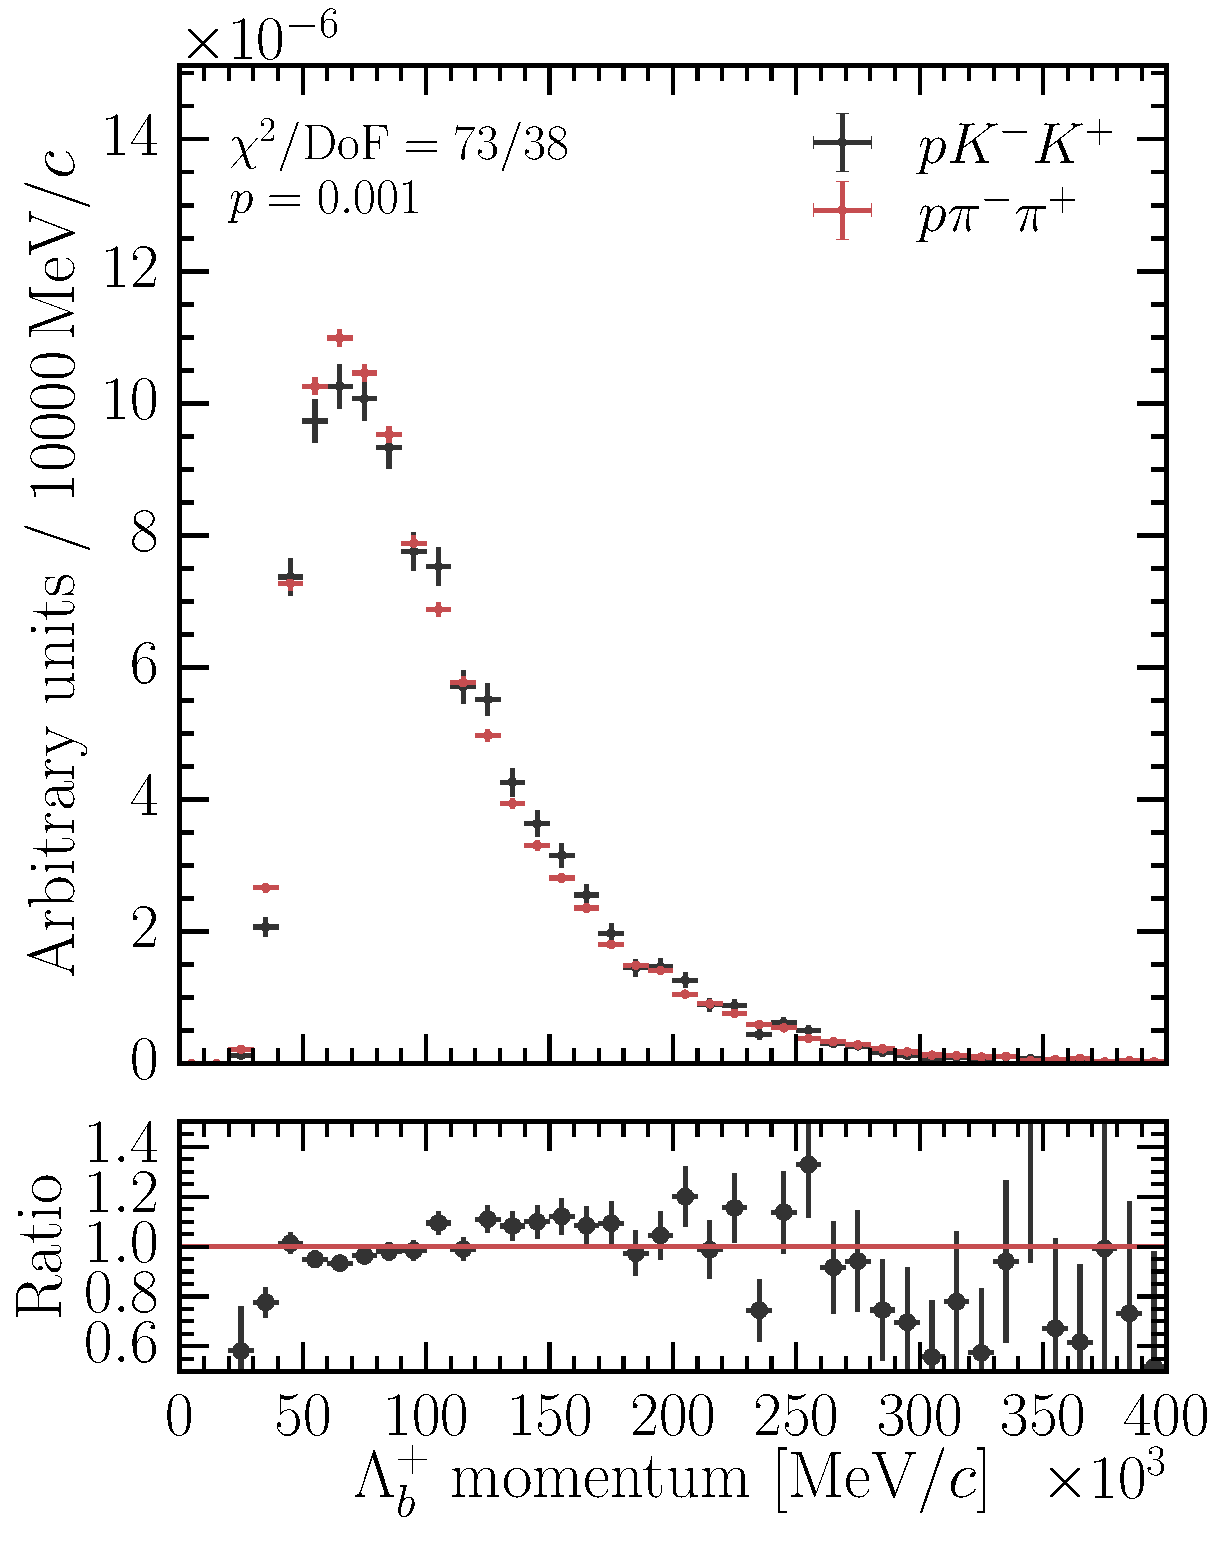
\includegraphics[width=\textwidth]{cpv/kinematic_weighting/preweighting_kinematics/LcToppipi_2012_MagDown_Lb_P}
    \label{fig:cpv:kinematic_weighting:pre:Lb:P}
  \end{subfigure}
  \begin{subfigure}[b]{0.4\textwidth}
    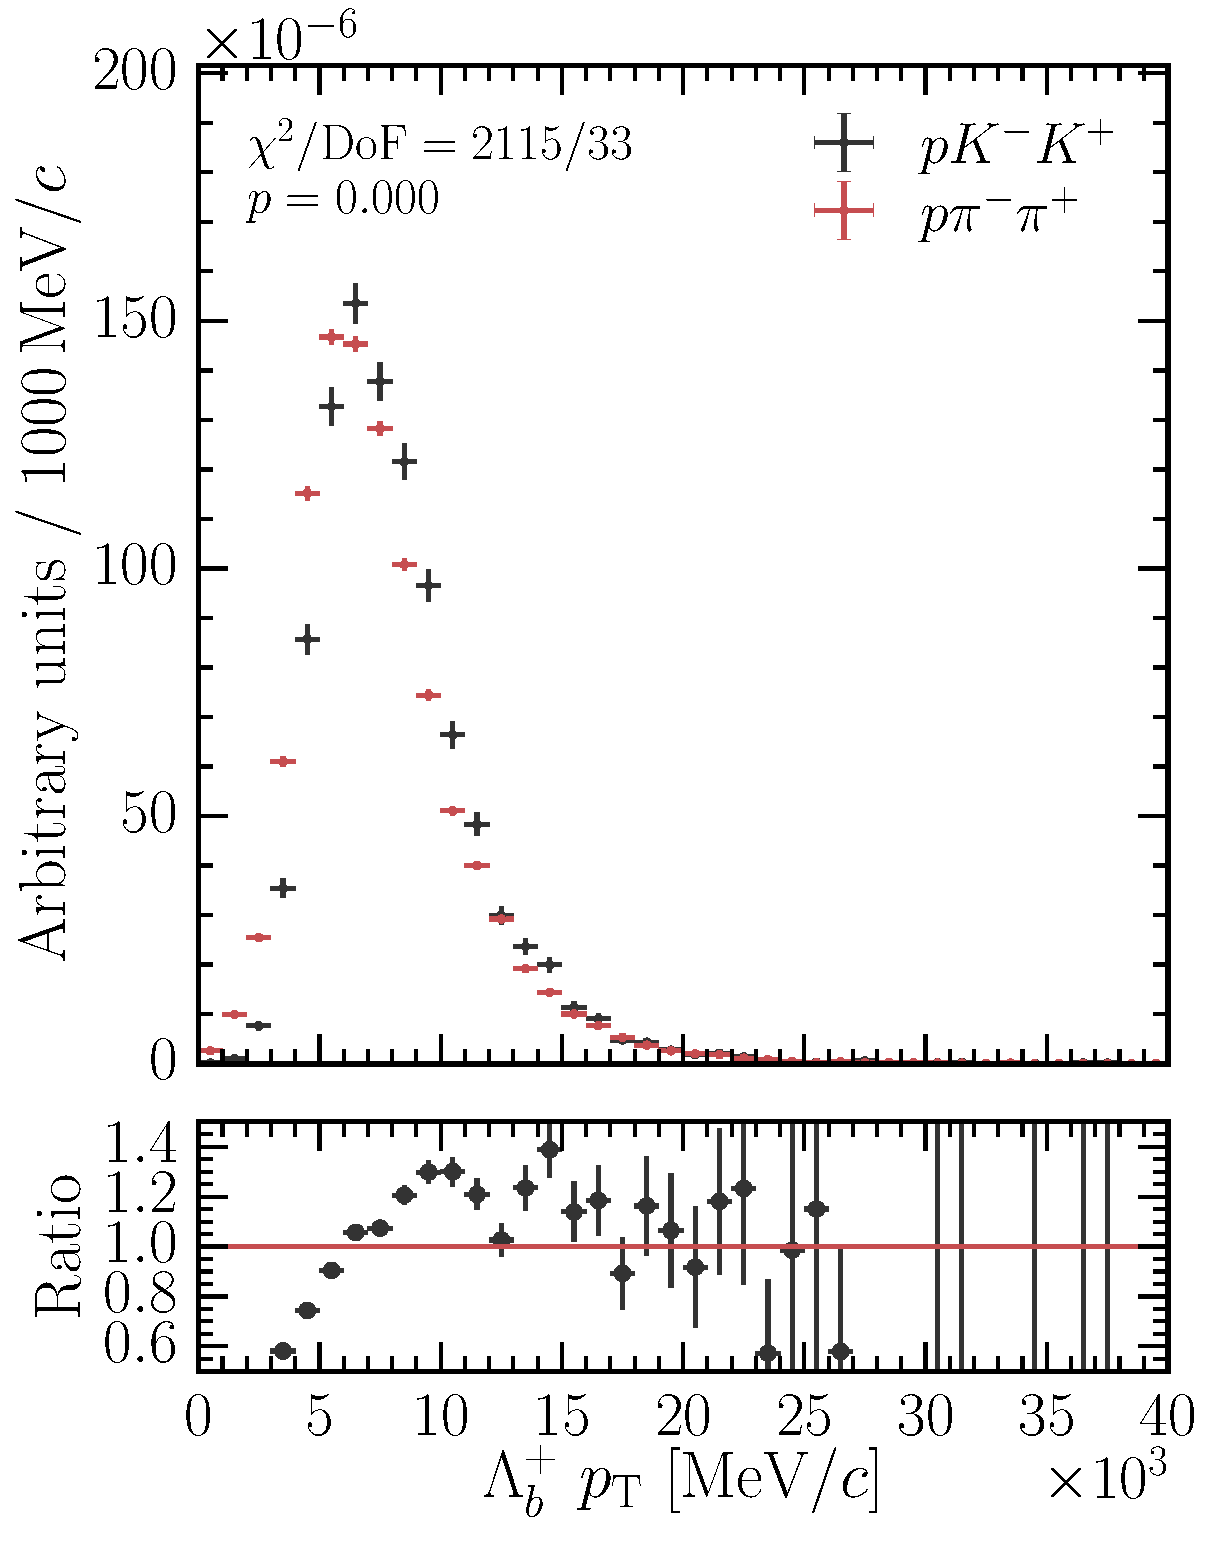
\includegraphics[width=\textwidth]{cpv/kinematic_weighting/preweighting_kinematics/LcToppipi_2012_MagDown_Lb_PT}
    \label{fig:cpv:kinematic_weighting:pre:Lb:PT}
  \end{subfigure}\\
  \begin{subfigure}[b]{0.4\textwidth}
    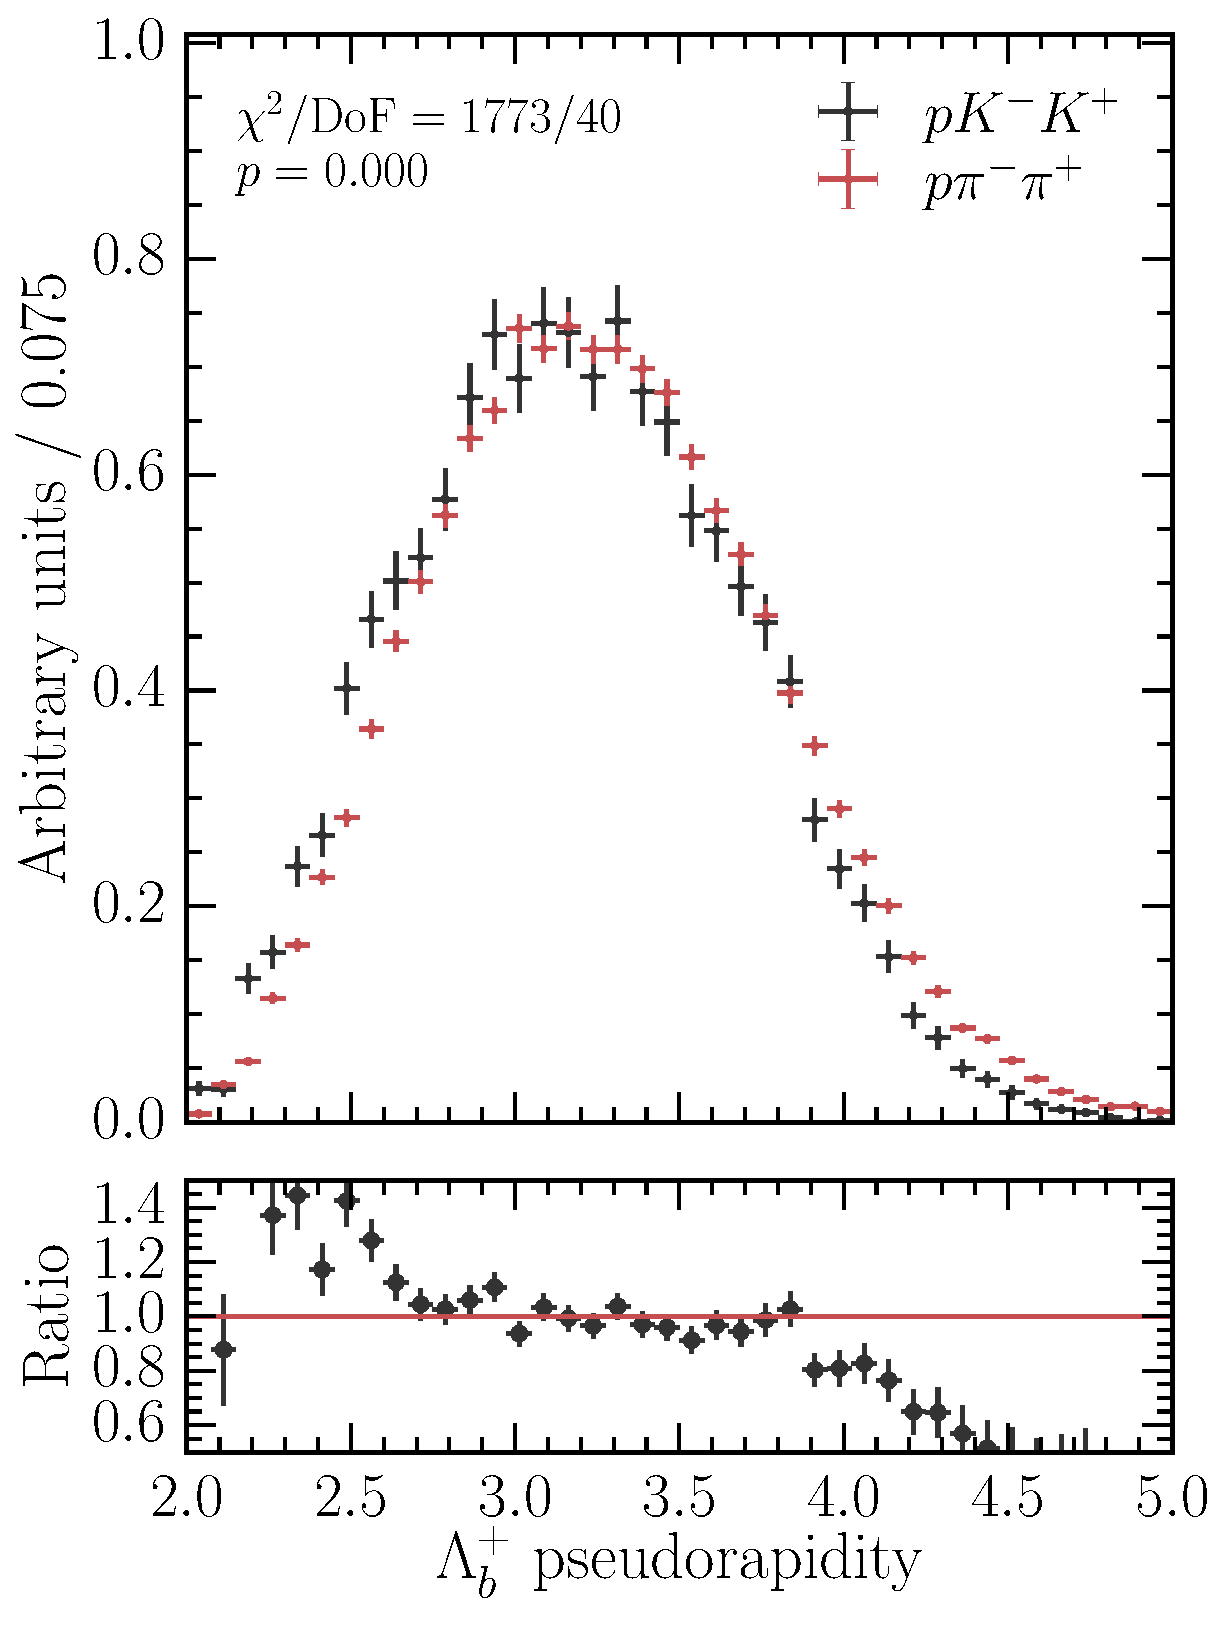
\includegraphics[width=\textwidth]{cpv/kinematic_weighting/preweighting_kinematics/LcToppipi_2012_MagDown_Lb_ETA}
    \label{fig:cpv:kinematic_weighting:pre:Lb:ETA}
  \end{subfigure}
  \begin{subfigure}[b]{0.4\textwidth}
    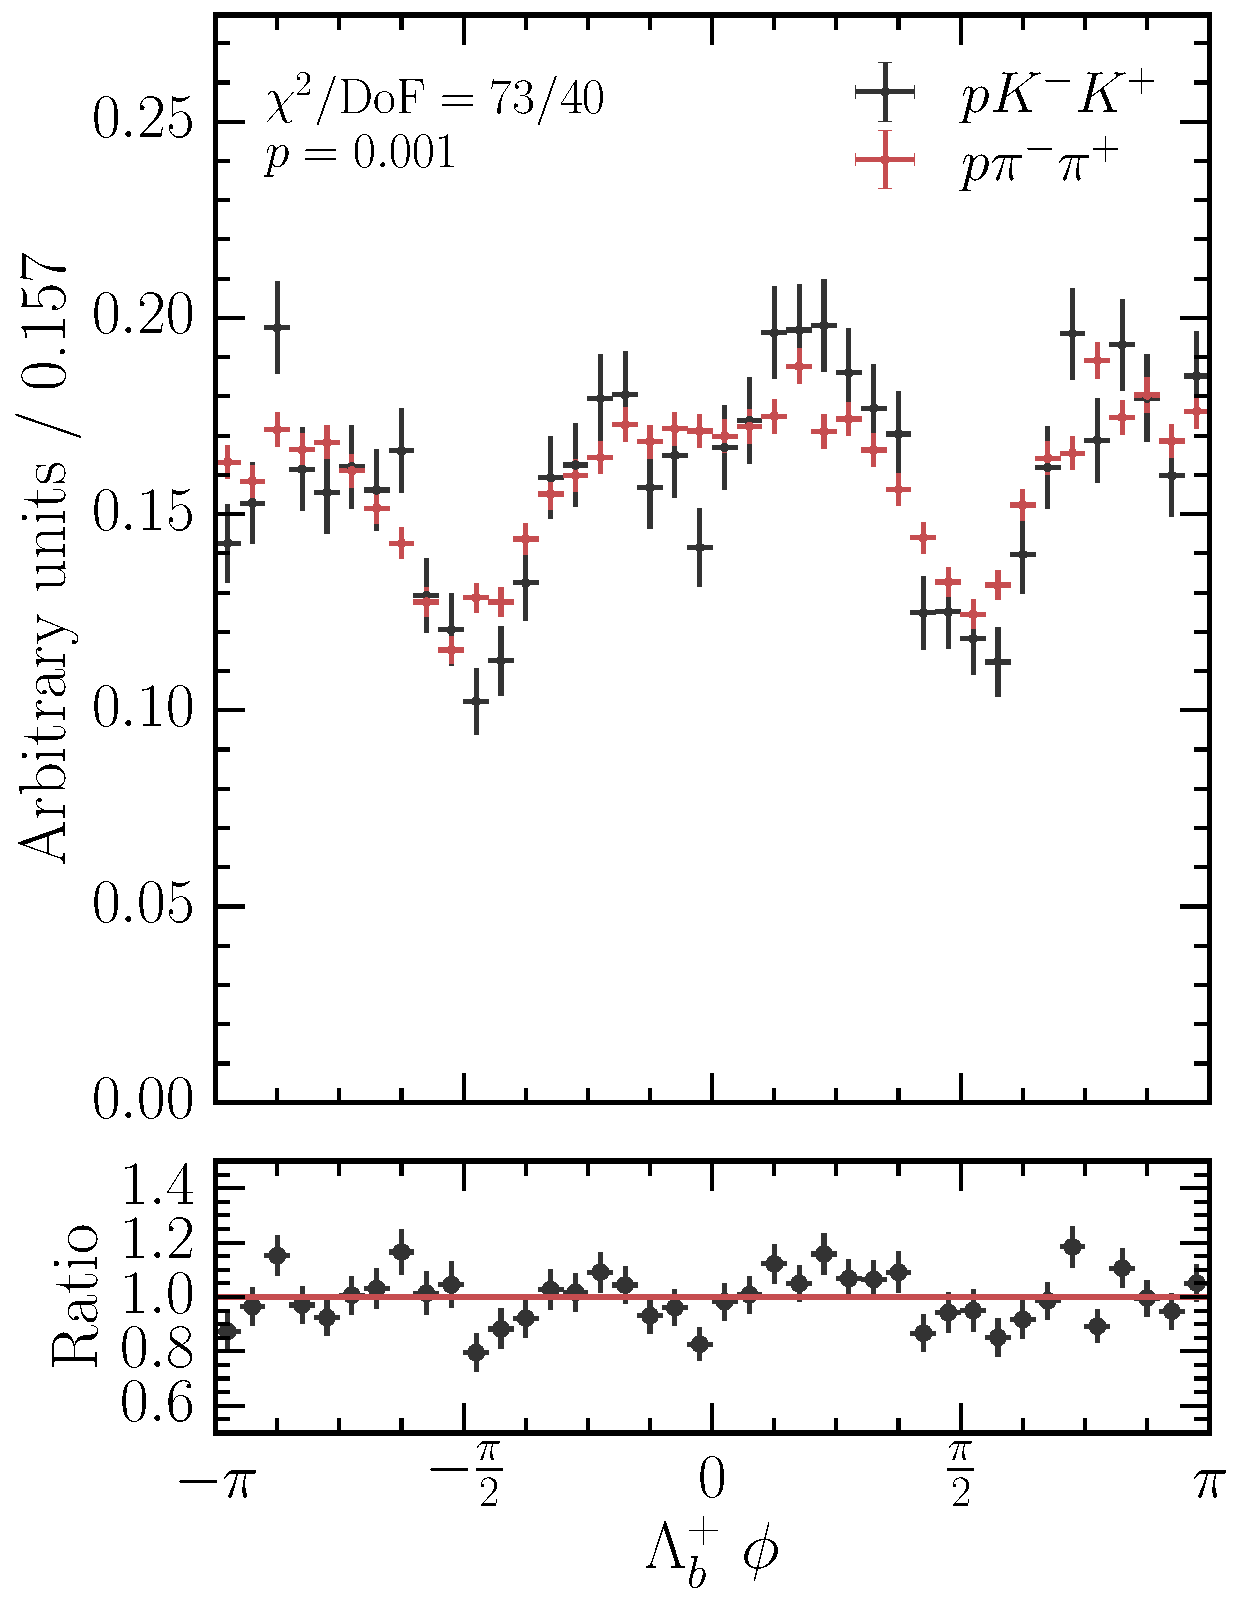
\includegraphics[width=\textwidth]{cpv/kinematic_weighting/preweighting_kinematics/LcToppipi_2012_MagDown_Lb_PHI}
    \label{fig:cpv:kinematic_weighting:pre:Lb:PHI}
  \end{subfigure}
  \caption{%
    Clockwise from the top left: total momentum, transverse momentum, angle 
    $\phi$, and pseudorapidity of the \PLambdab, weighted by signal sWeights.
    The 2012 magnet down data is shown.
  }
  \label{fig:cpv:kinematic_weighting:pre:Lb}
\end{figure}

\begin{figure}
  \begin{subfigure}[b]{0.4\textwidth}
    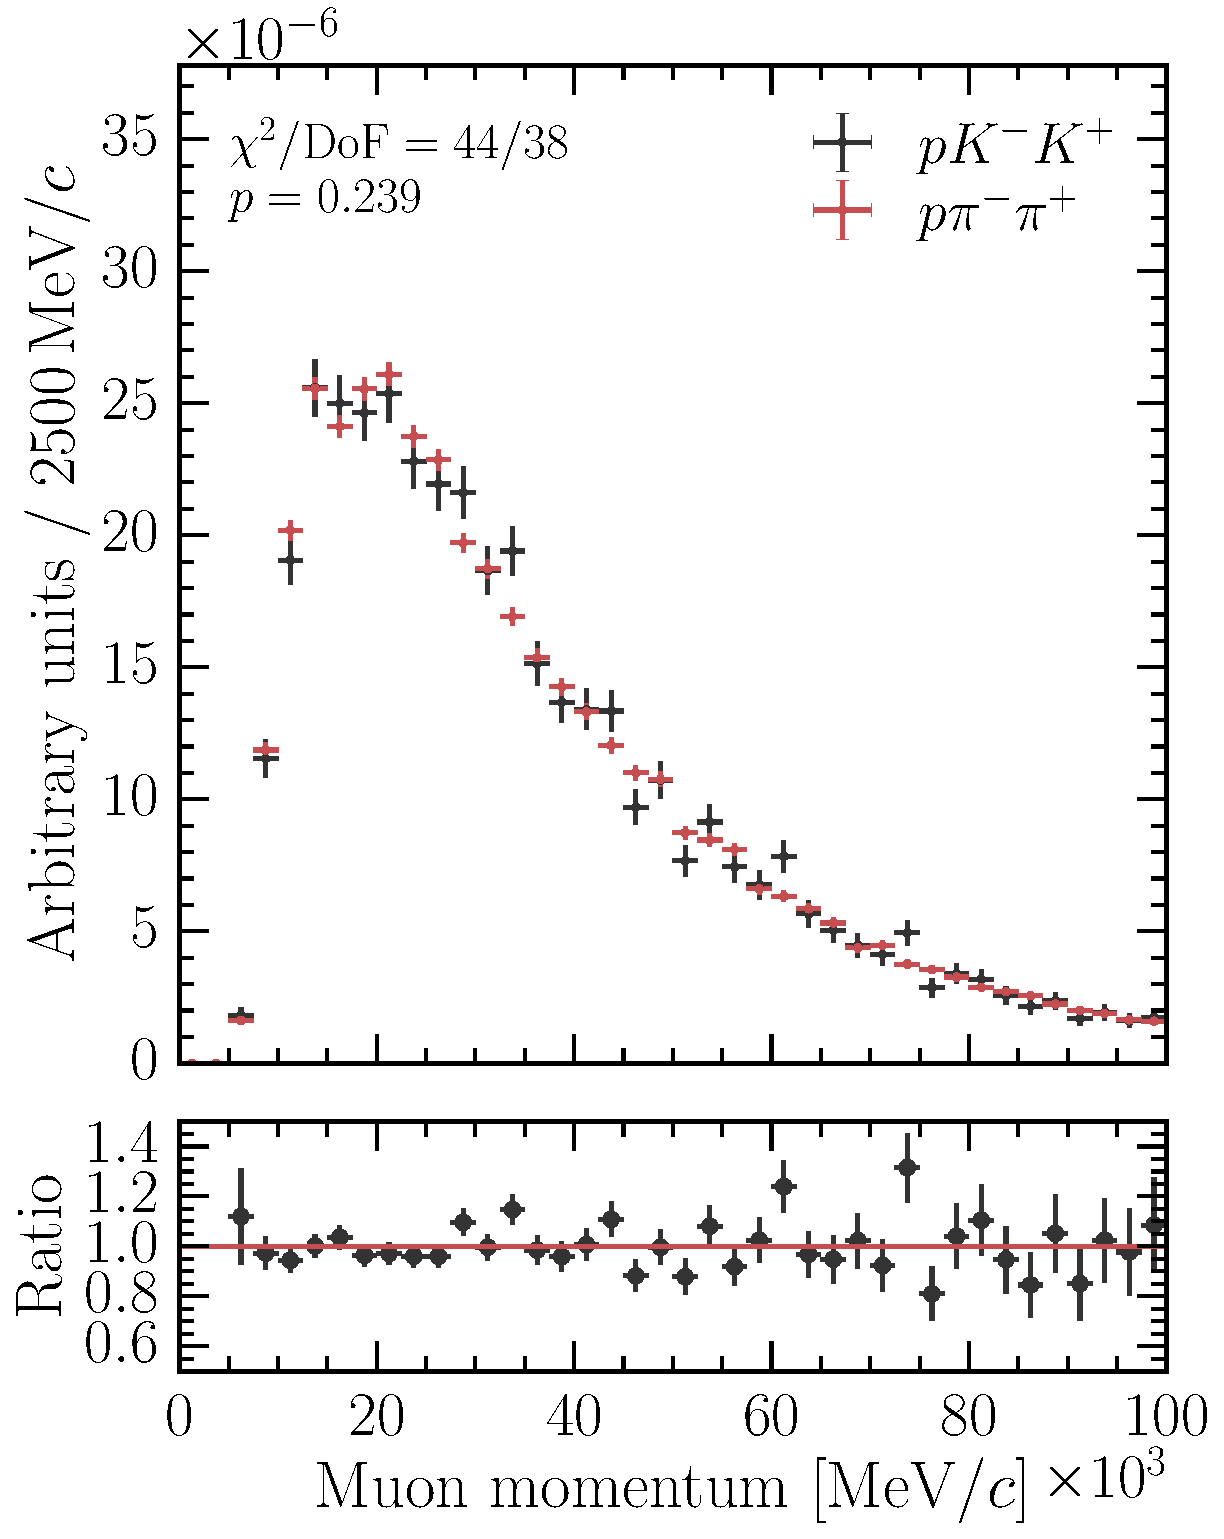
\includegraphics[width=\textwidth]{cpv/kinematic_weighting/preweighting_kinematics/LcToppipi_2012_MagDown_Lb_mu_P}
    \label{fig:cpv:kinematic_weighting:pre:Lb_mu:P}
  \end{subfigure}
  \begin{subfigure}[b]{0.4\textwidth}
    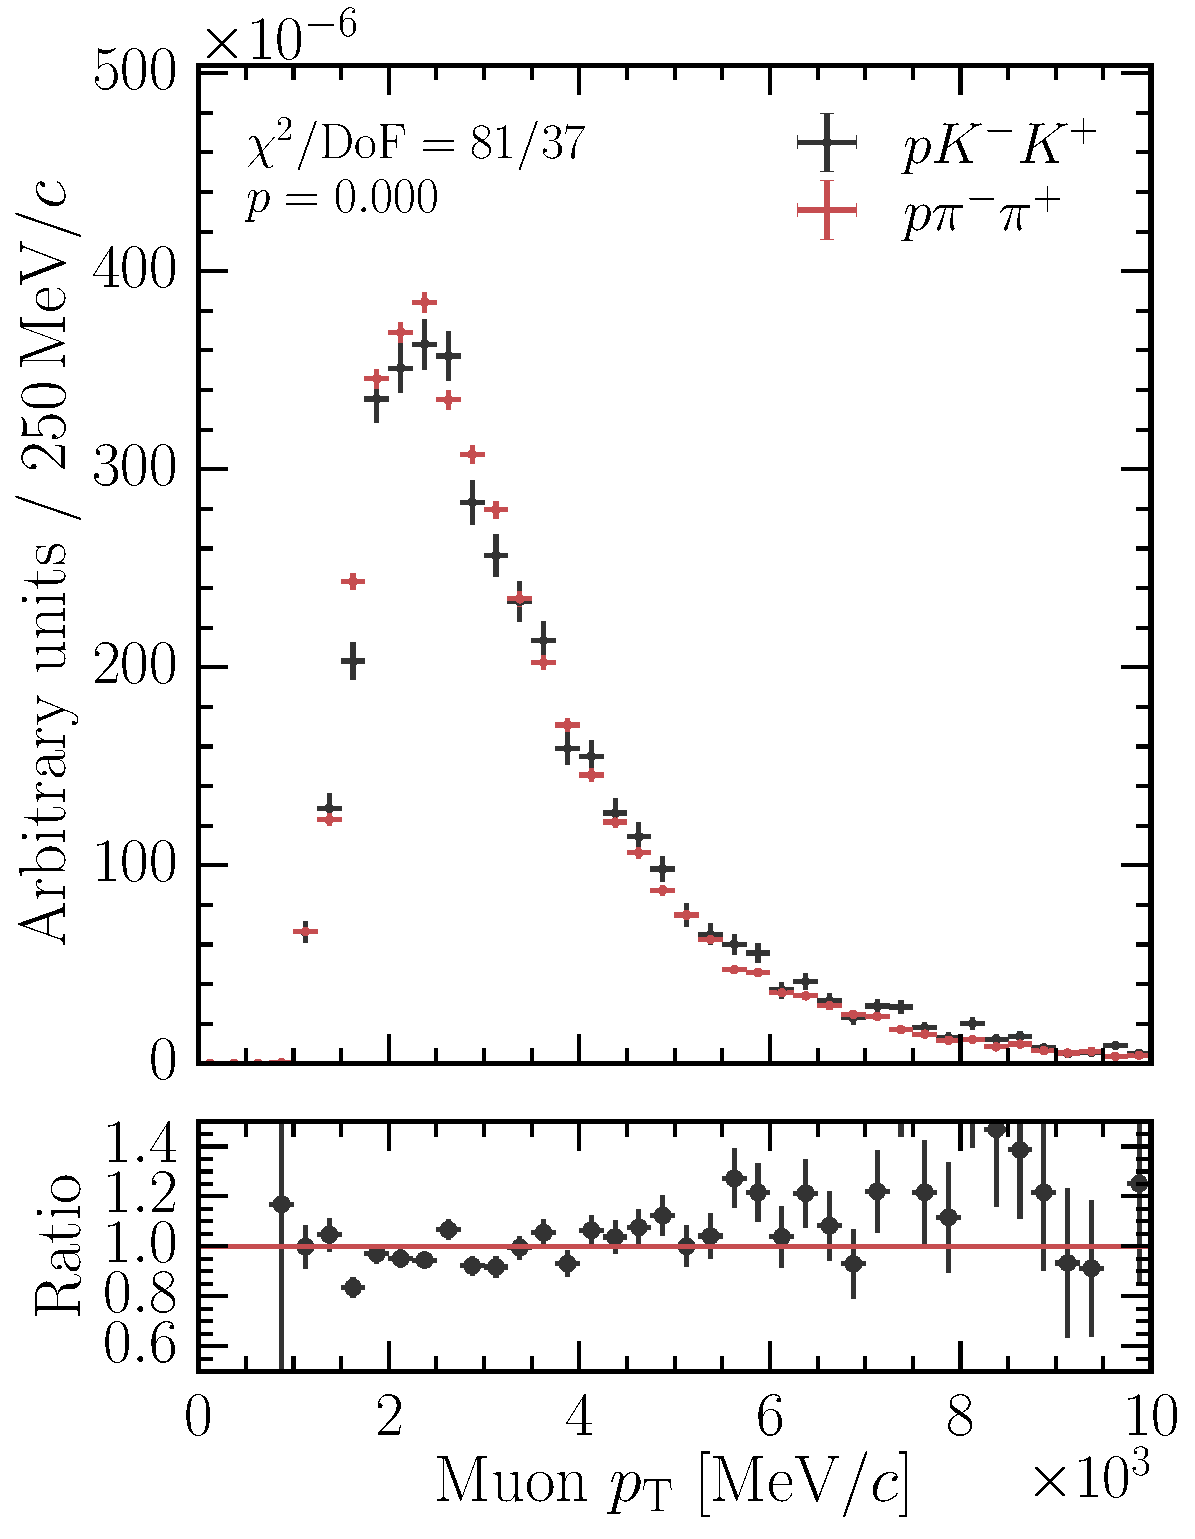
\includegraphics[width=\textwidth]{cpv/kinematic_weighting/preweighting_kinematics/LcToppipi_2012_MagDown_Lb_mu_PT}
    \label{fig:cpv:kinematic_weighting:pre:Lb_mu:PT}
  \end{subfigure}\\
  \begin{subfigure}[b]{0.4\textwidth}
    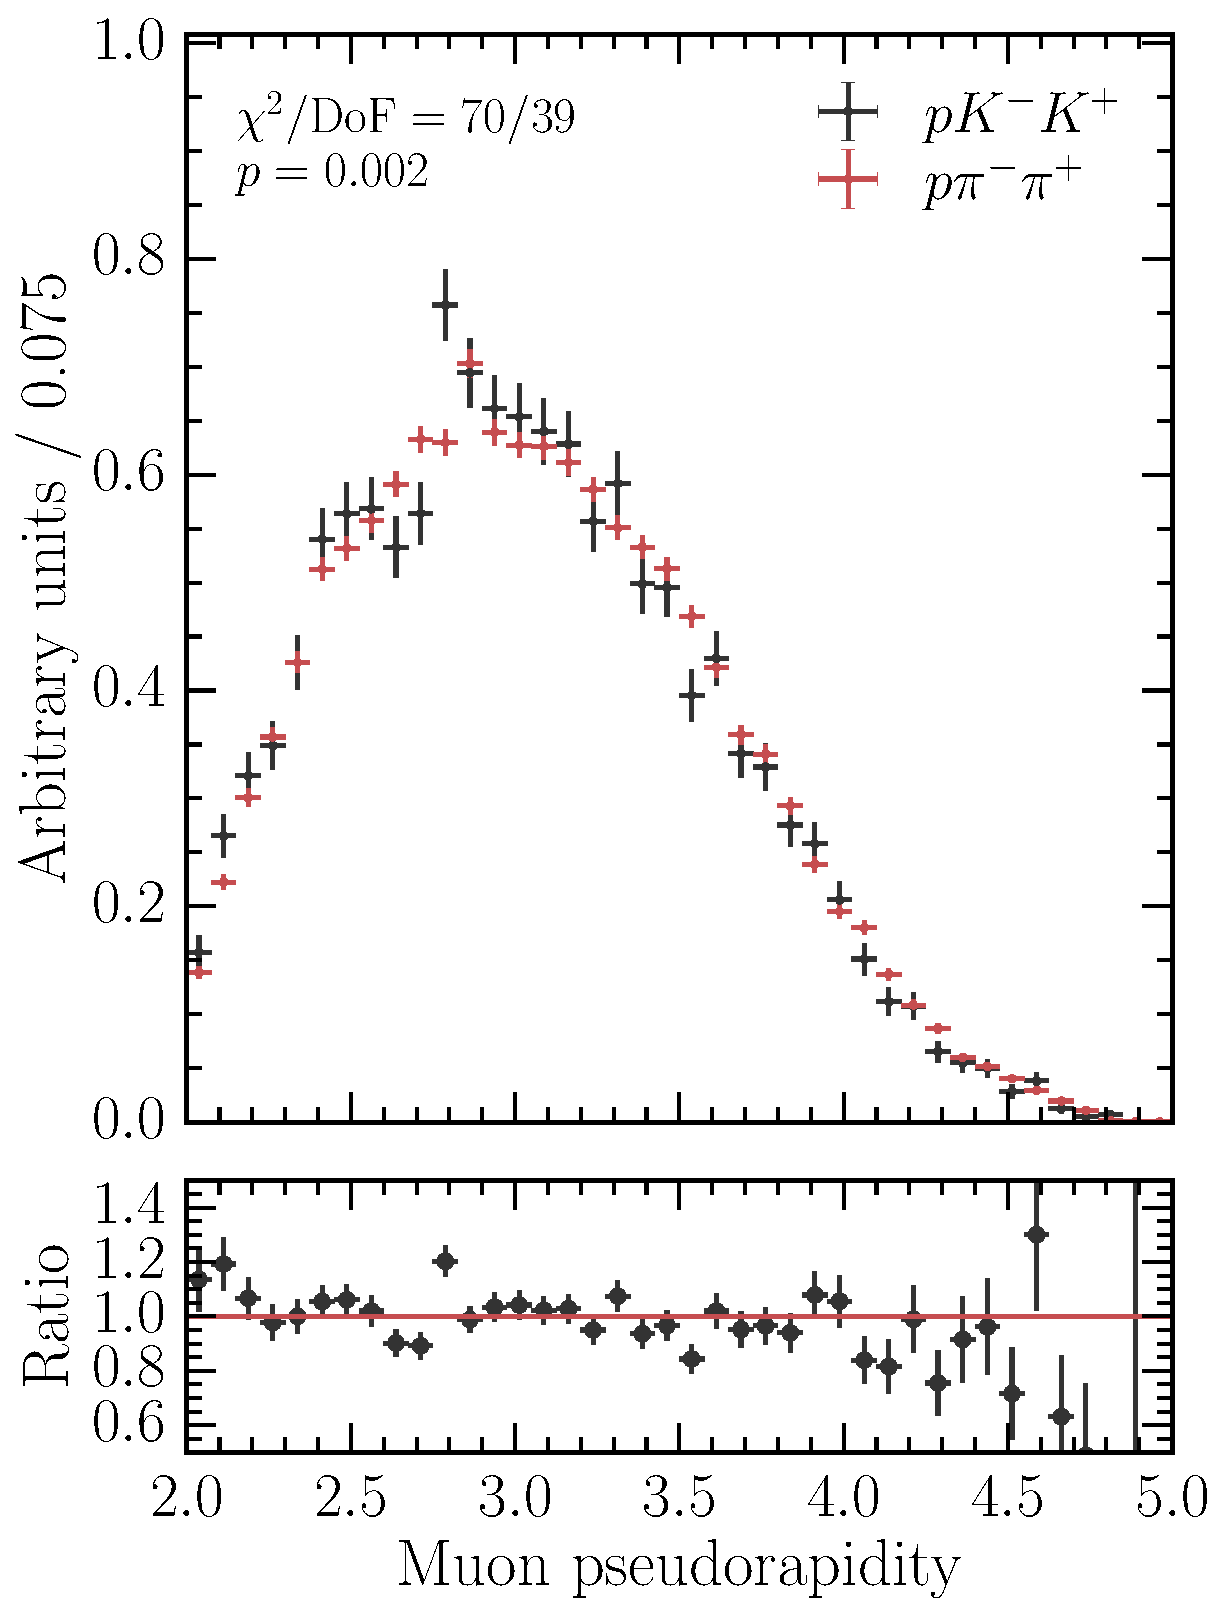
\includegraphics[width=\textwidth]{cpv/kinematic_weighting/preweighting_kinematics/LcToppipi_2012_MagDown_Lb_mu_ETA}
    \label{fig:cpv:kinematic_weighting:pre:Lb_mu:ETA}
  \end{subfigure}
  \begin{subfigure}[b]{0.4\textwidth}
    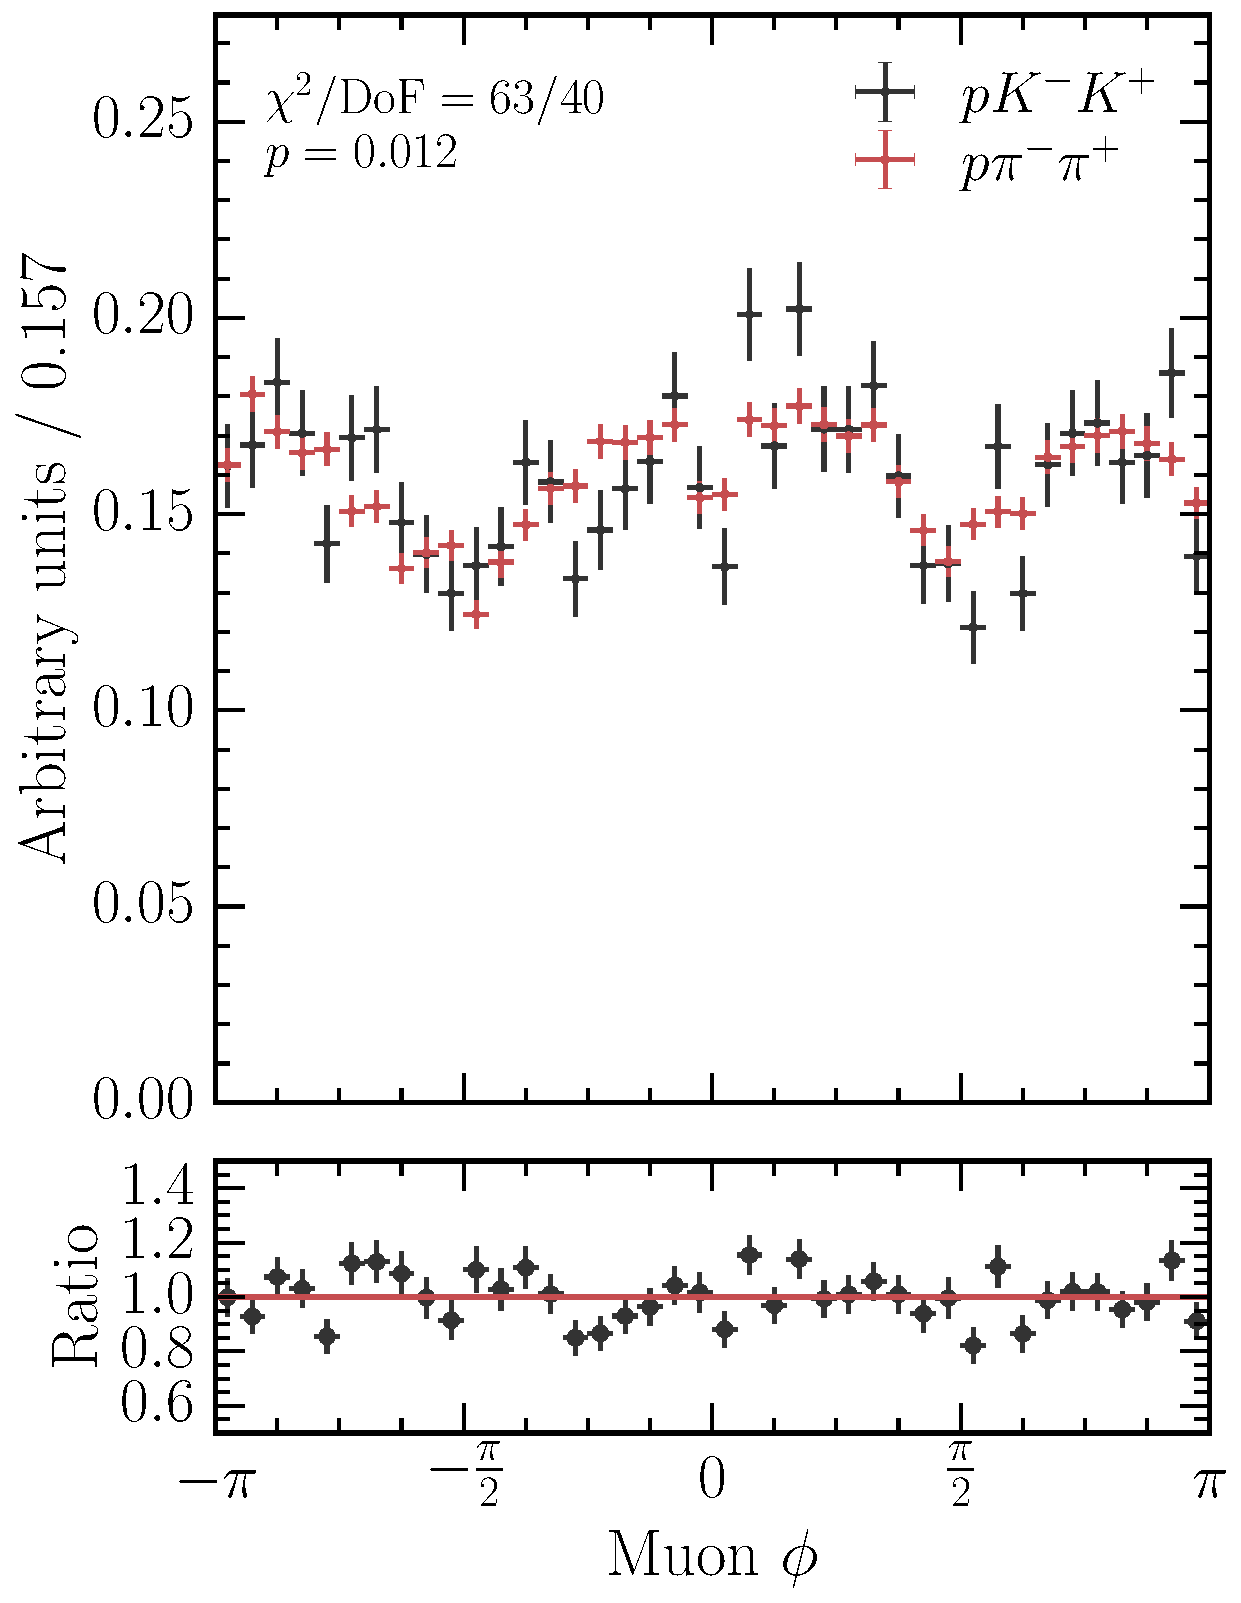
\includegraphics[width=\textwidth]{cpv/kinematic_weighting/preweighting_kinematics/LcToppipi_2012_MagDown_Lb_mu_PHI}
    \label{fig:cpv:kinematic_weighting:pre:Lb_mu:PHI}
  \end{subfigure}
  \caption{%
    Clockwise from the top left: total momentum, transverse momentum, angle 
    $\phi$, and pseudorapidity of the muon from the \PLambdab, weighted by 
    signal sWeights.
    The 2012 magnet down data is shown.
  }
  \label{fig:cpv:kinematic_weighting:pre:Lb_mu}
\end{figure}

\begin{figure}
  \begin{subfigure}[b]{0.4\textwidth}
    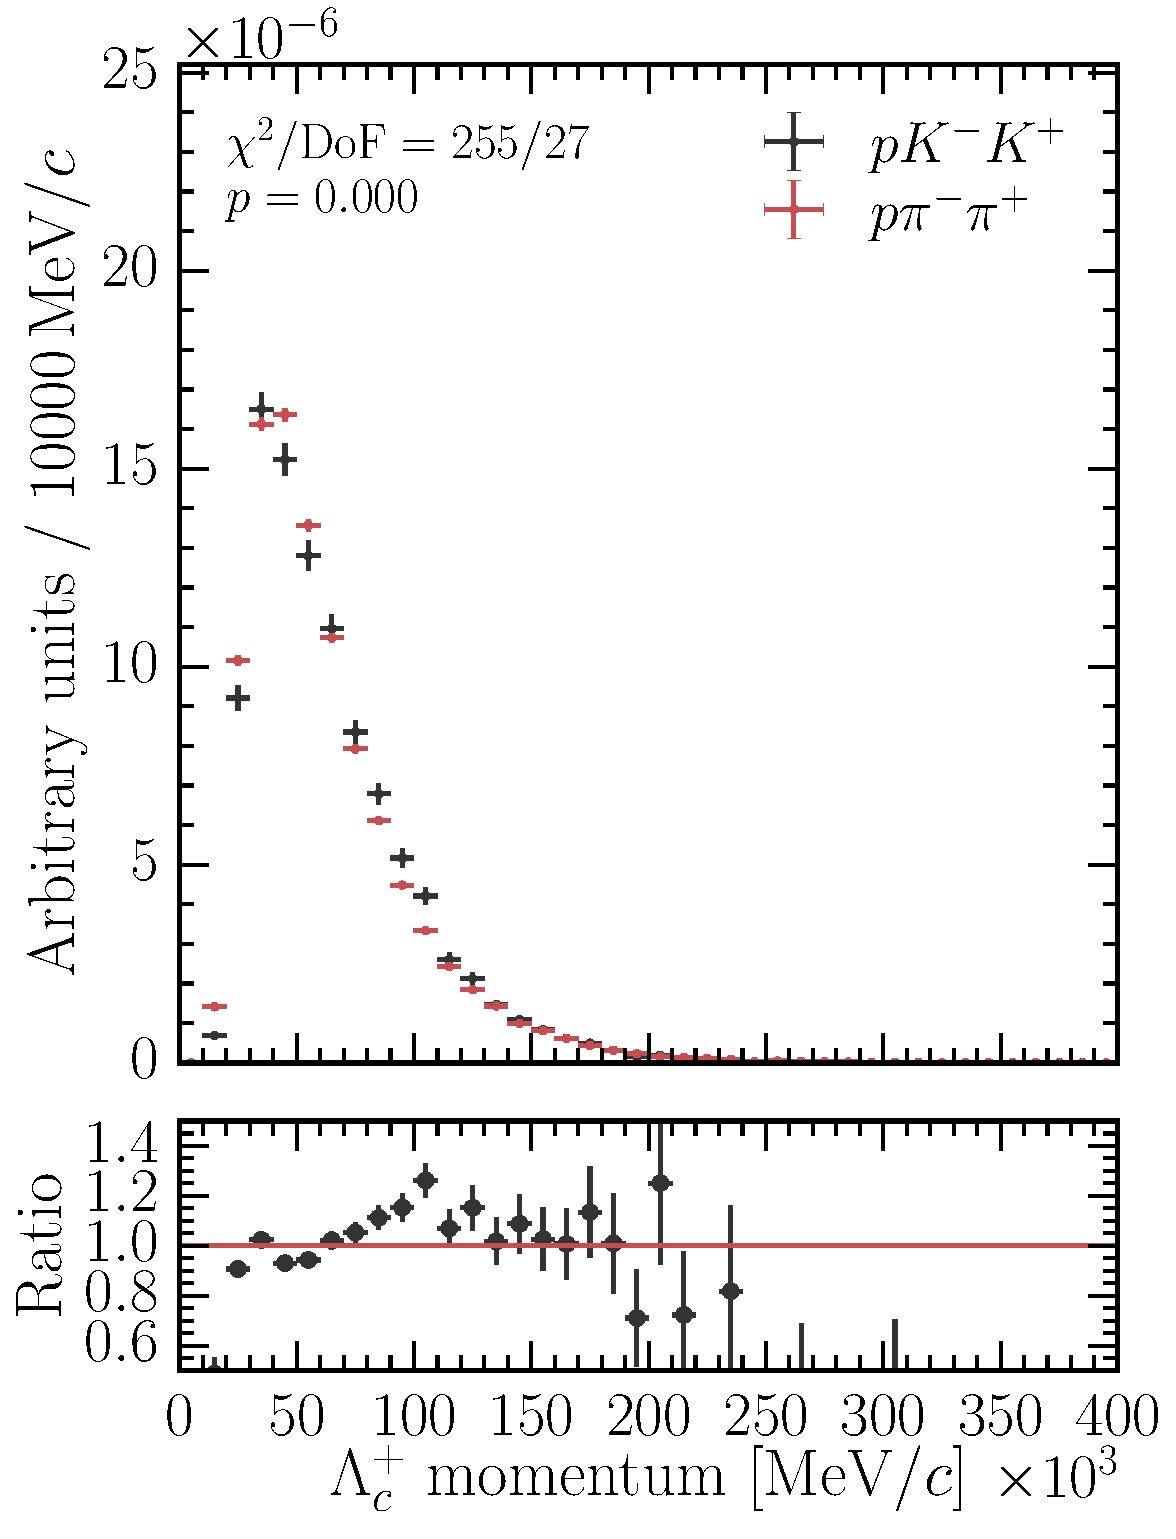
\includegraphics[width=\textwidth]{cpv/kinematic_weighting/preweighting_kinematics/LcToppipi_2012_MagDown_Lc_P}
    \label{fig:cpv:kinematic_weighting:pre:Lc:P}
  \end{subfigure}
  \begin{subfigure}[b]{0.4\textwidth}
    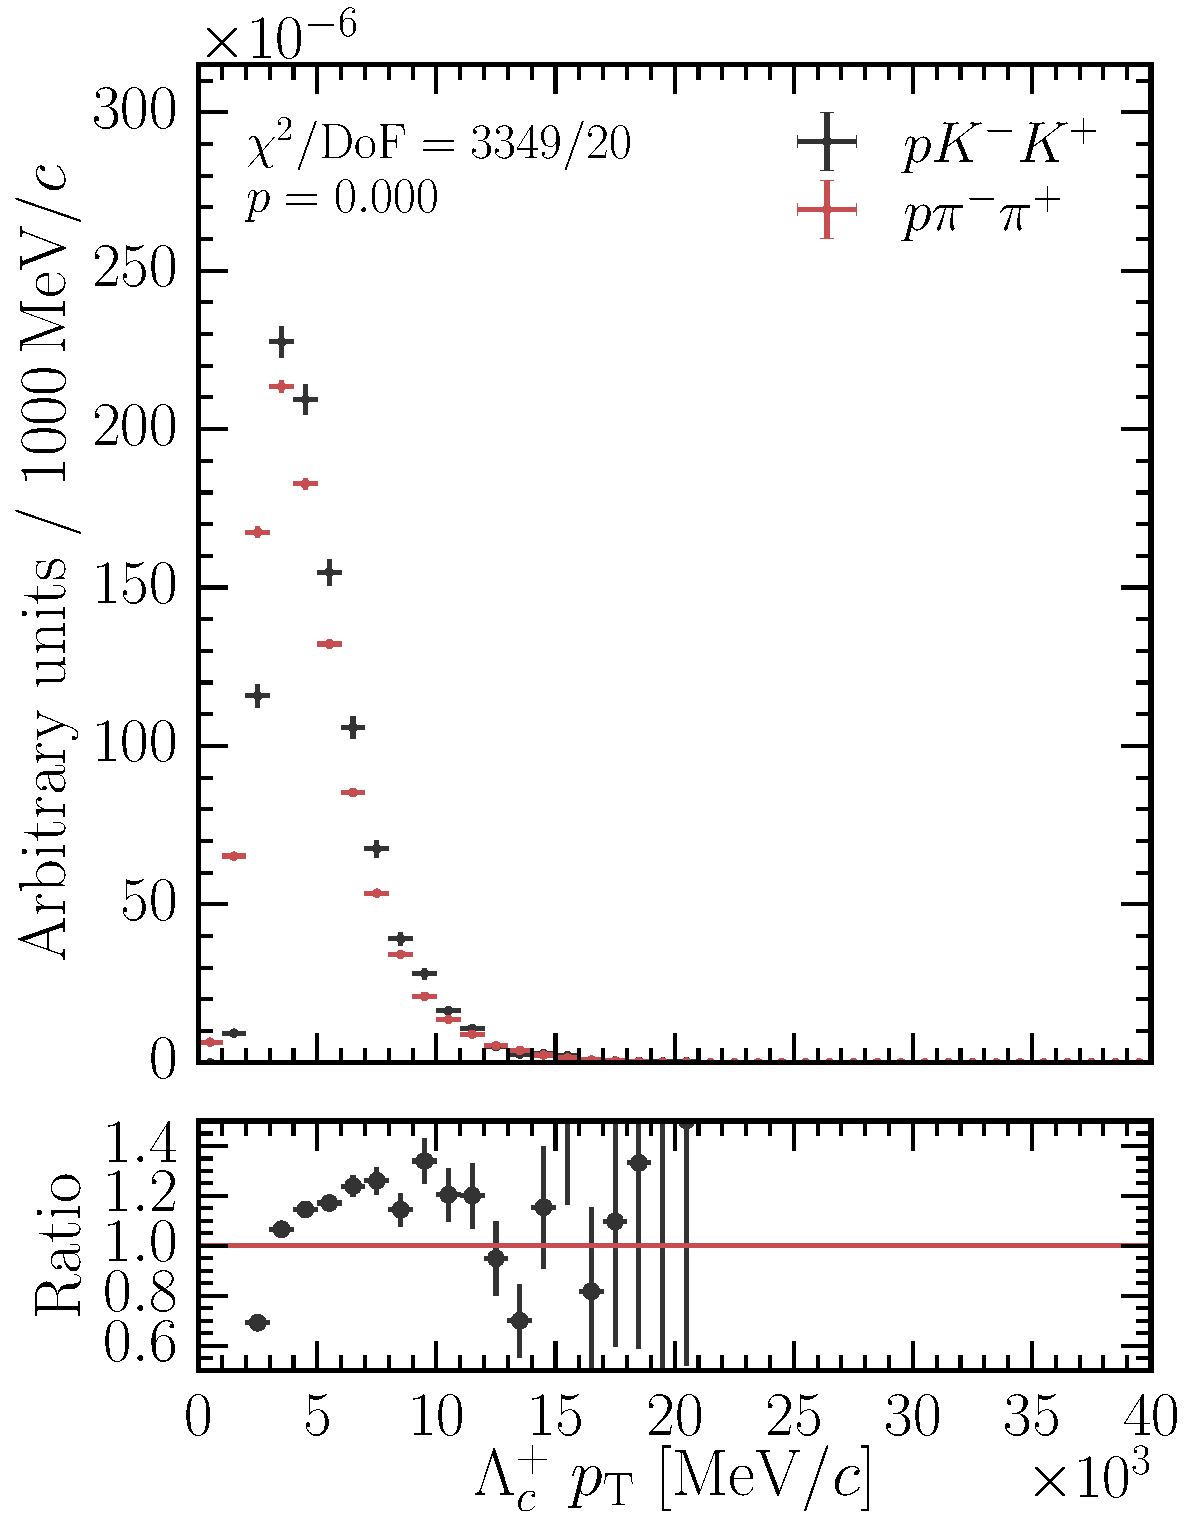
\includegraphics[width=\textwidth]{cpv/kinematic_weighting/preweighting_kinematics/LcToppipi_2012_MagDown_Lc_PT}
    \label{fig:cpv:kinematic_weighting:pre:Lc:PT}
  \end{subfigure}\\
  \begin{subfigure}[b]{0.4\textwidth}
    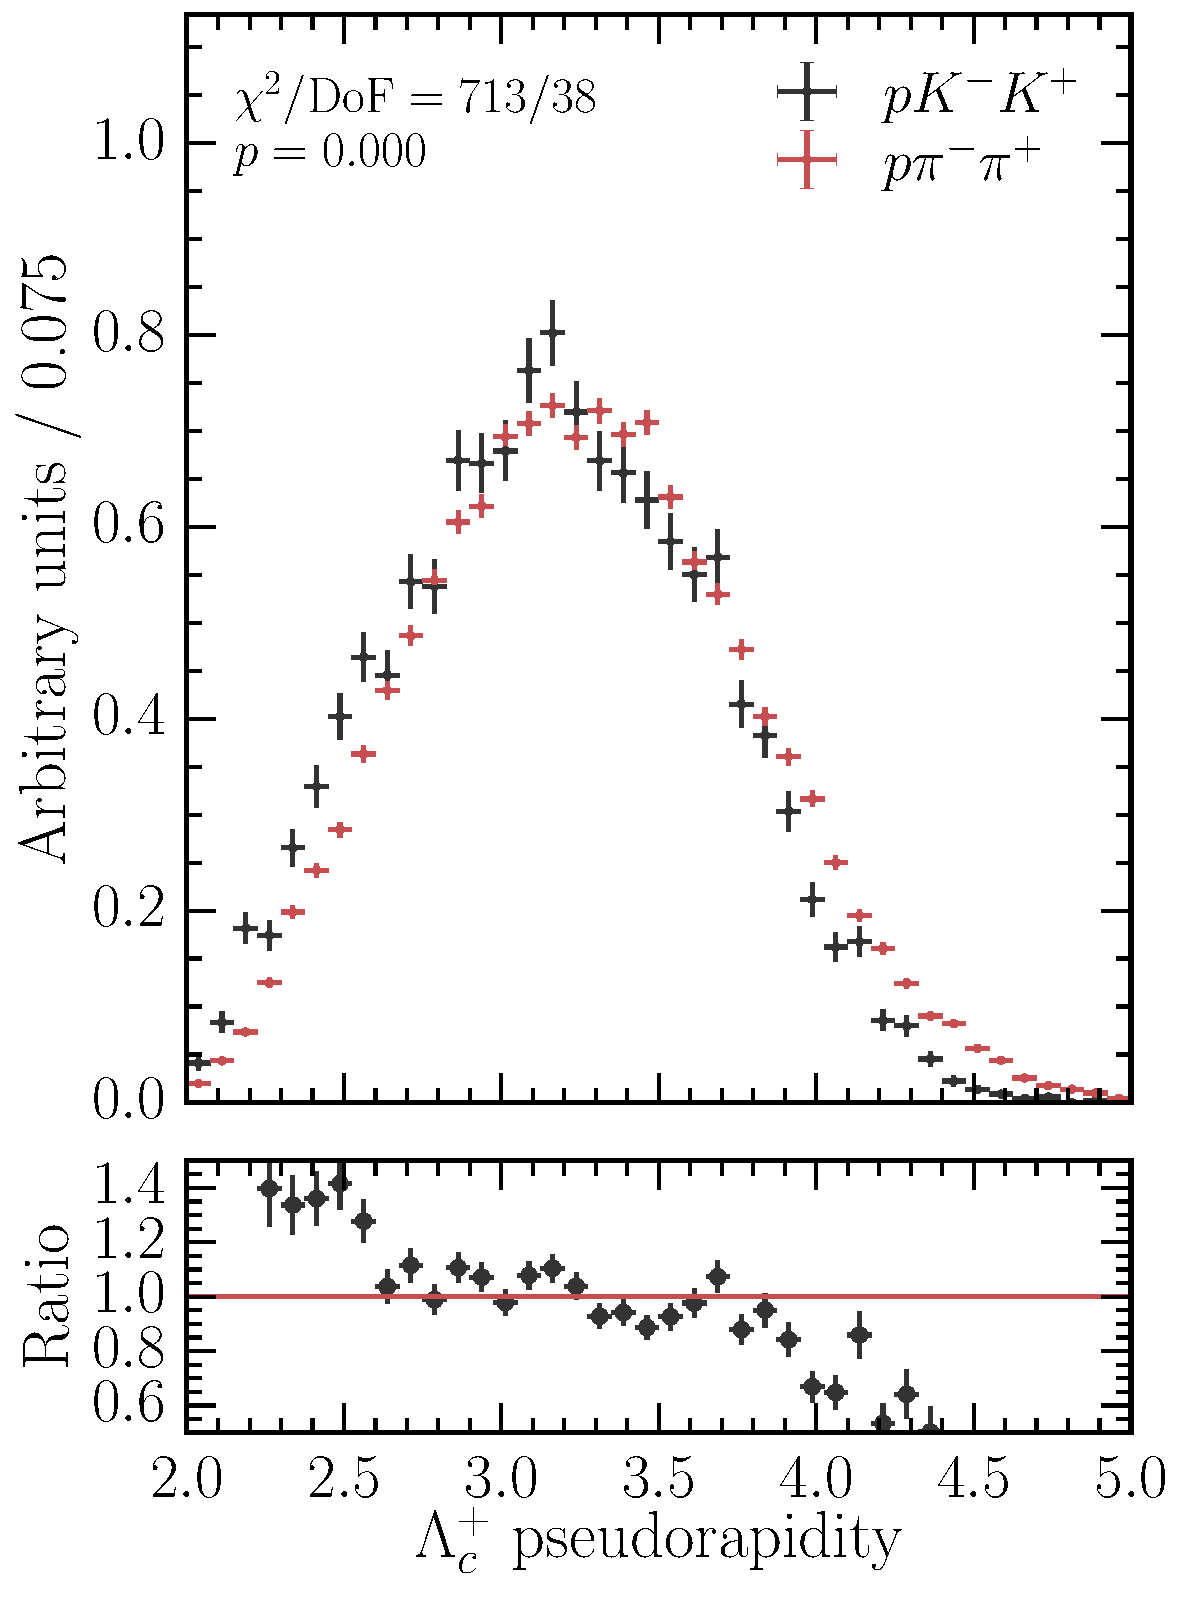
\includegraphics[width=\textwidth]{cpv/kinematic_weighting/preweighting_kinematics/LcToppipi_2012_MagDown_Lc_ETA}
    \label{fig:cpv:kinematic_weighting:pre:Lc:ETA}
  \end{subfigure}
  \begin{subfigure}[b]{0.4\textwidth}
    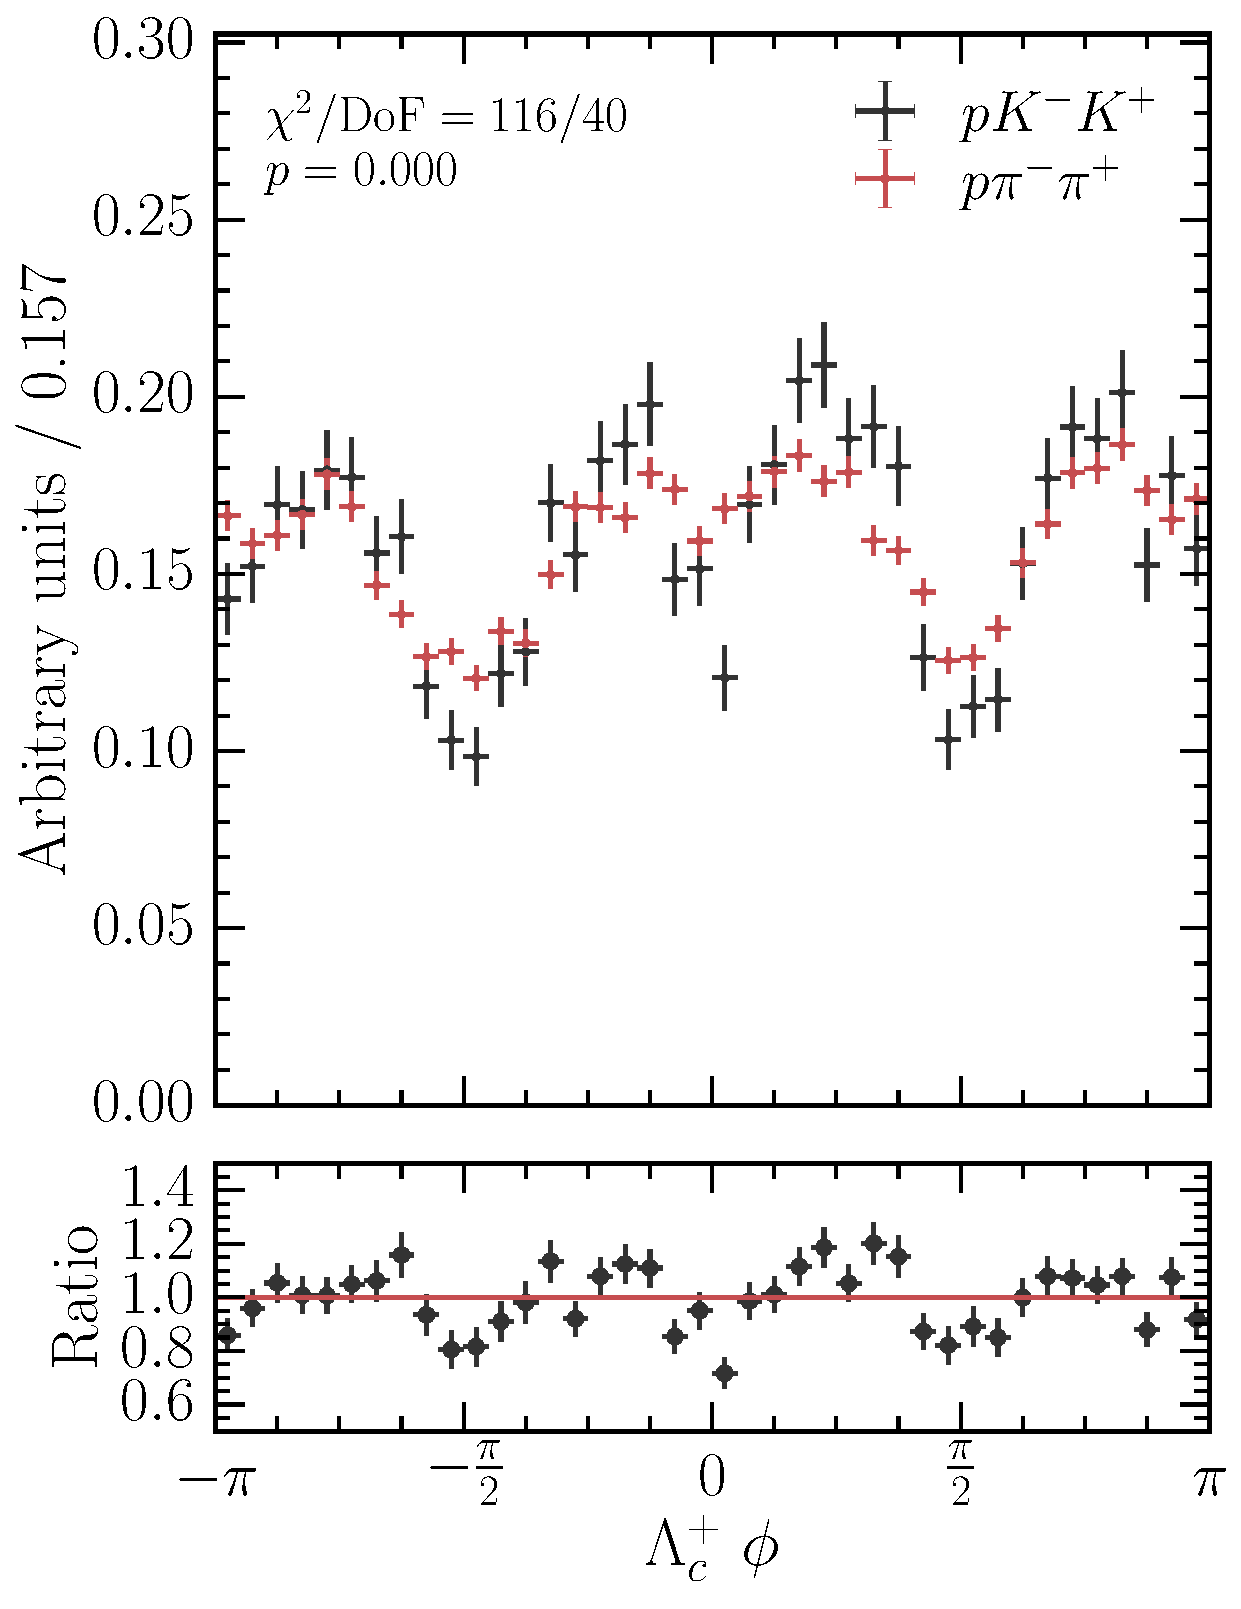
\includegraphics[width=\textwidth]{cpv/kinematic_weighting/preweighting_kinematics/LcToppipi_2012_MagDown_Lc_PHI}
    \label{fig:cpv:kinematic_weighting:pre:Lc:PHI}
  \end{subfigure}
  \caption{%
    Clockwise from the top left: total momentum, transverse momentum, angle 
    $\phi$, and pseudorapidity of the \PLambdac, weighted by signal sWeights.
    The 2012 magnet down data is shown.
  }
  \label{fig:cpv:kinematic_weighting:pre:Lc}
\end{figure}

\begin{figure}
  \begin{subfigure}[b]{0.4\textwidth}
    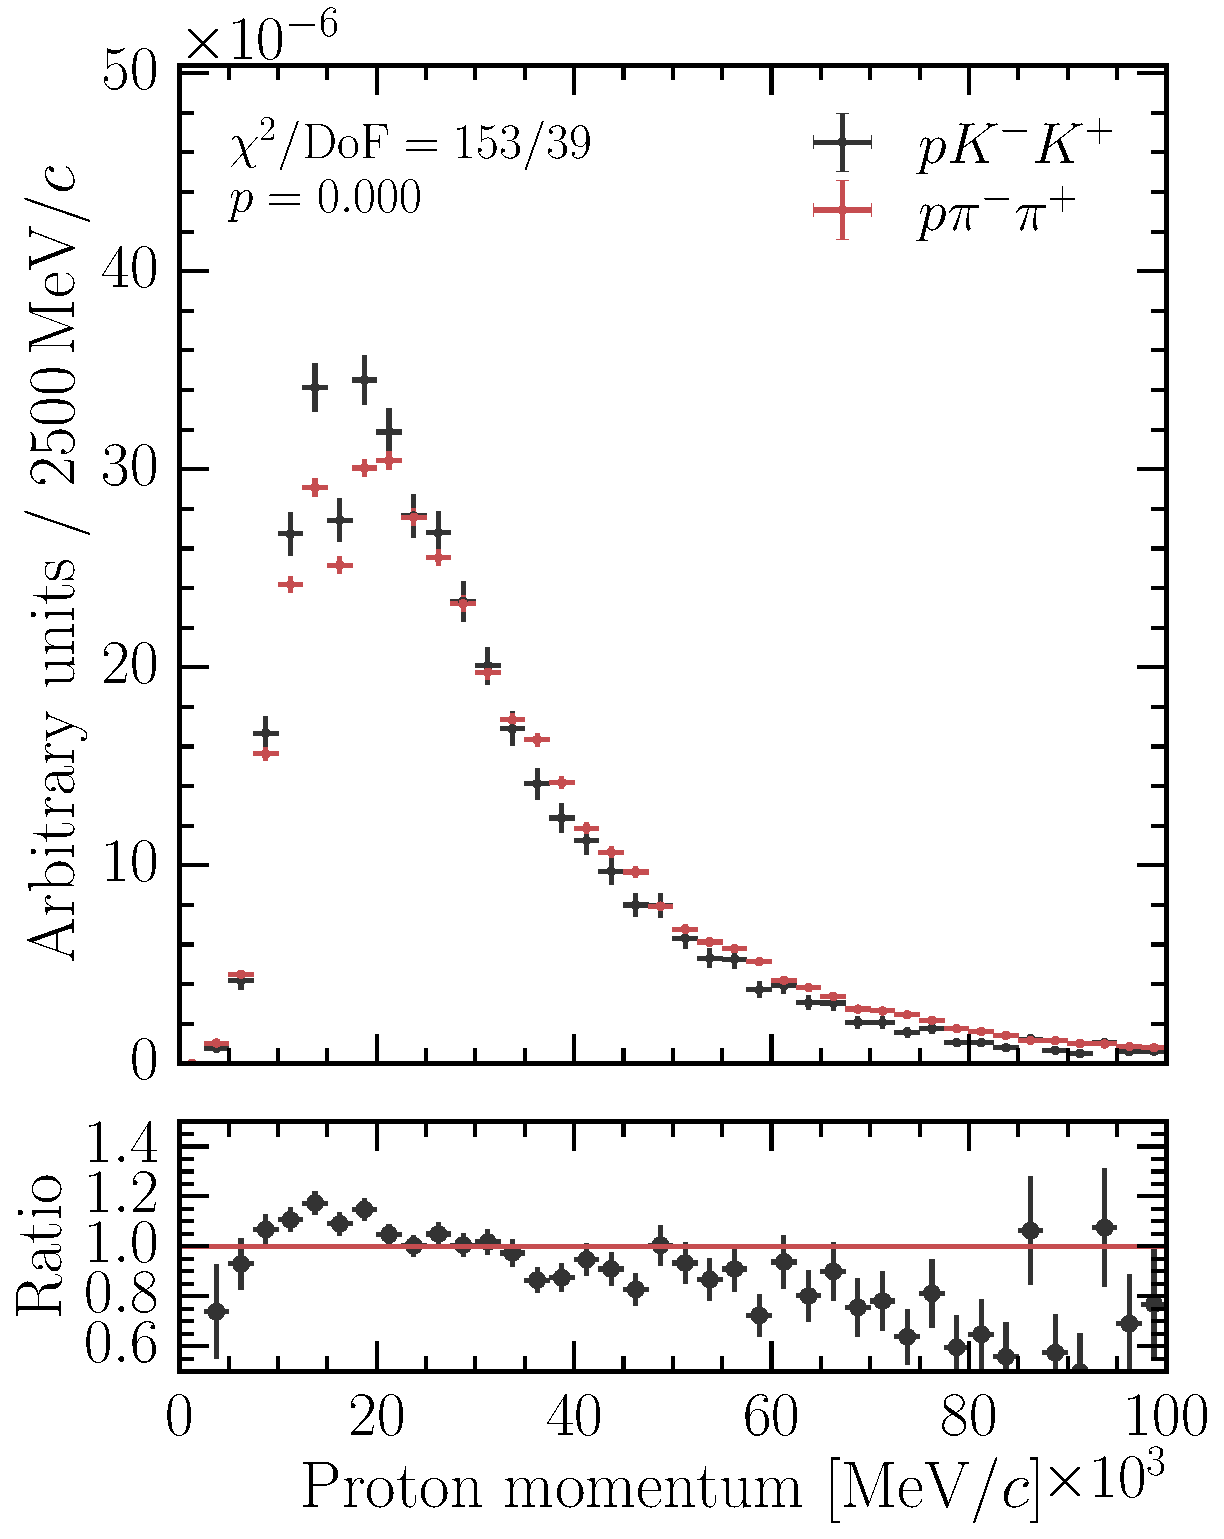
\includegraphics[width=\textwidth]{cpv/kinematic_weighting/preweighting_kinematics/LcToppipi_2012_MagDown_Lc_p_P}
    \label{fig:cpv:kinematic_weighting:pre:Lc_p:P}
  \end{subfigure}
  \begin{subfigure}[b]{0.4\textwidth}
    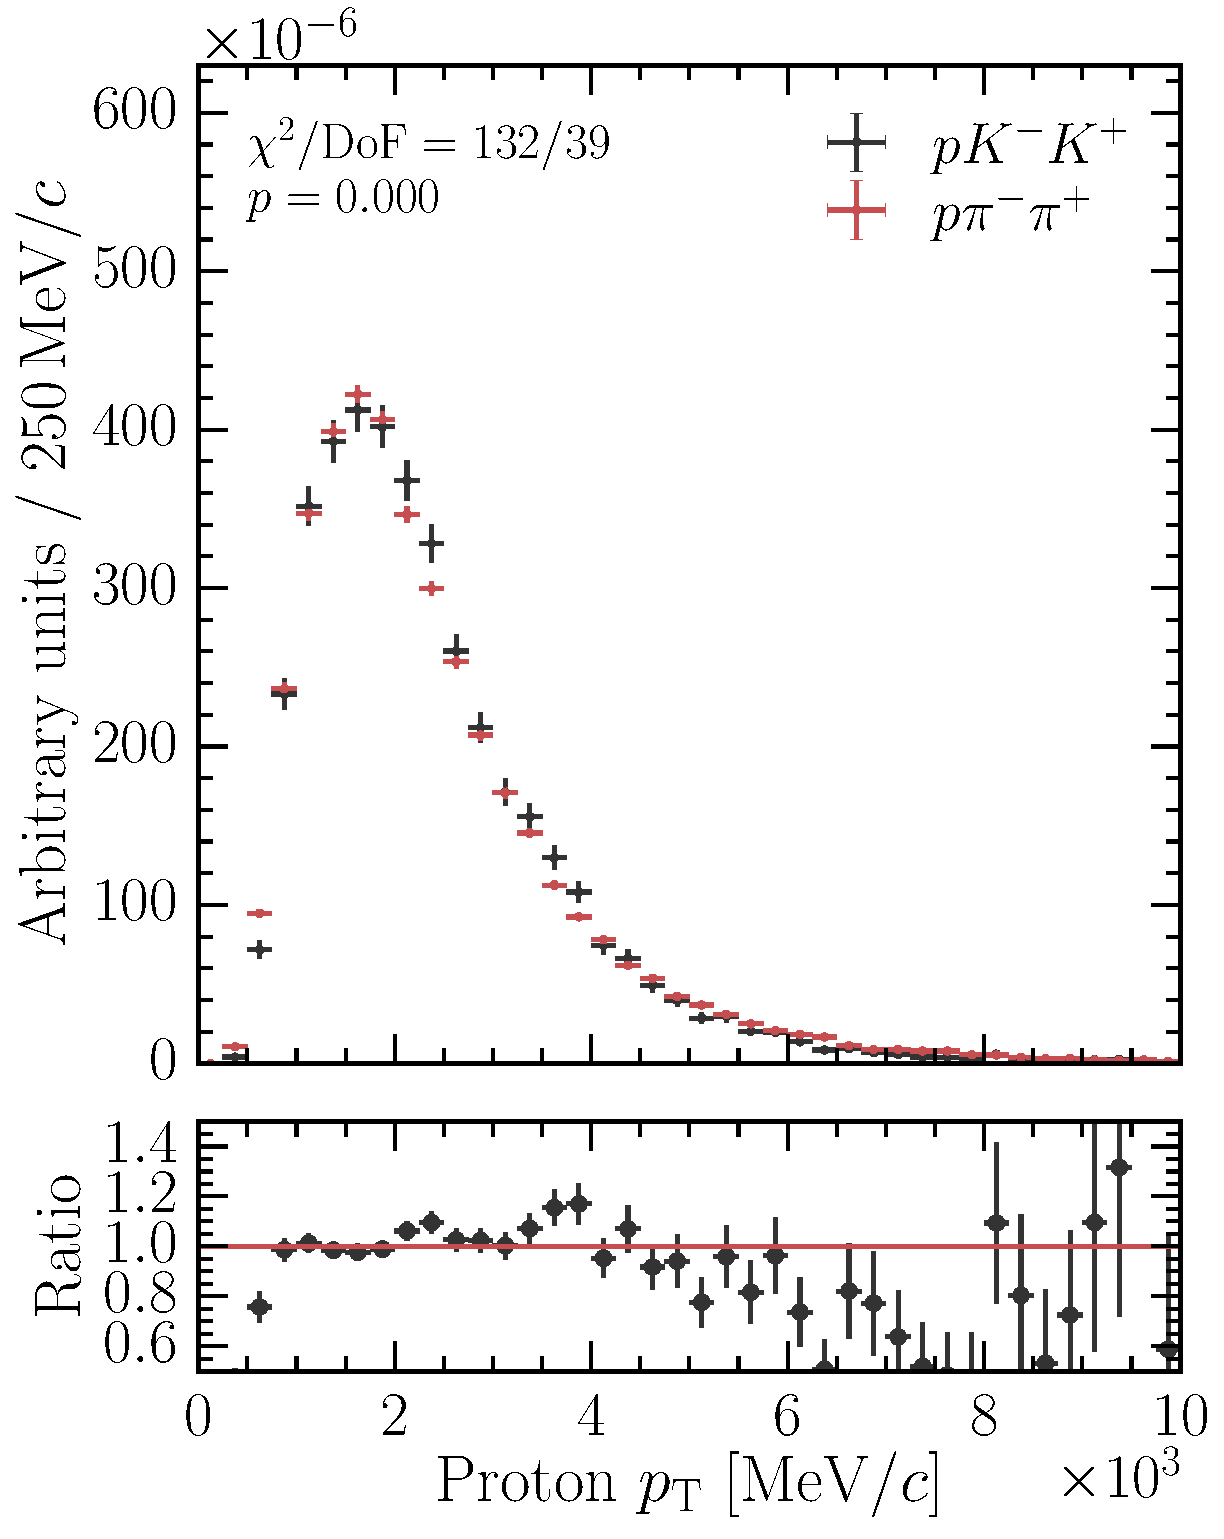
\includegraphics[width=\textwidth]{cpv/kinematic_weighting/preweighting_kinematics/LcToppipi_2012_MagDown_Lc_p_PT}
    \label{fig:cpv:kinematic_weighting:pre:Lc_p:PT}
  \end{subfigure}\\
  \begin{subfigure}[b]{0.4\textwidth}
    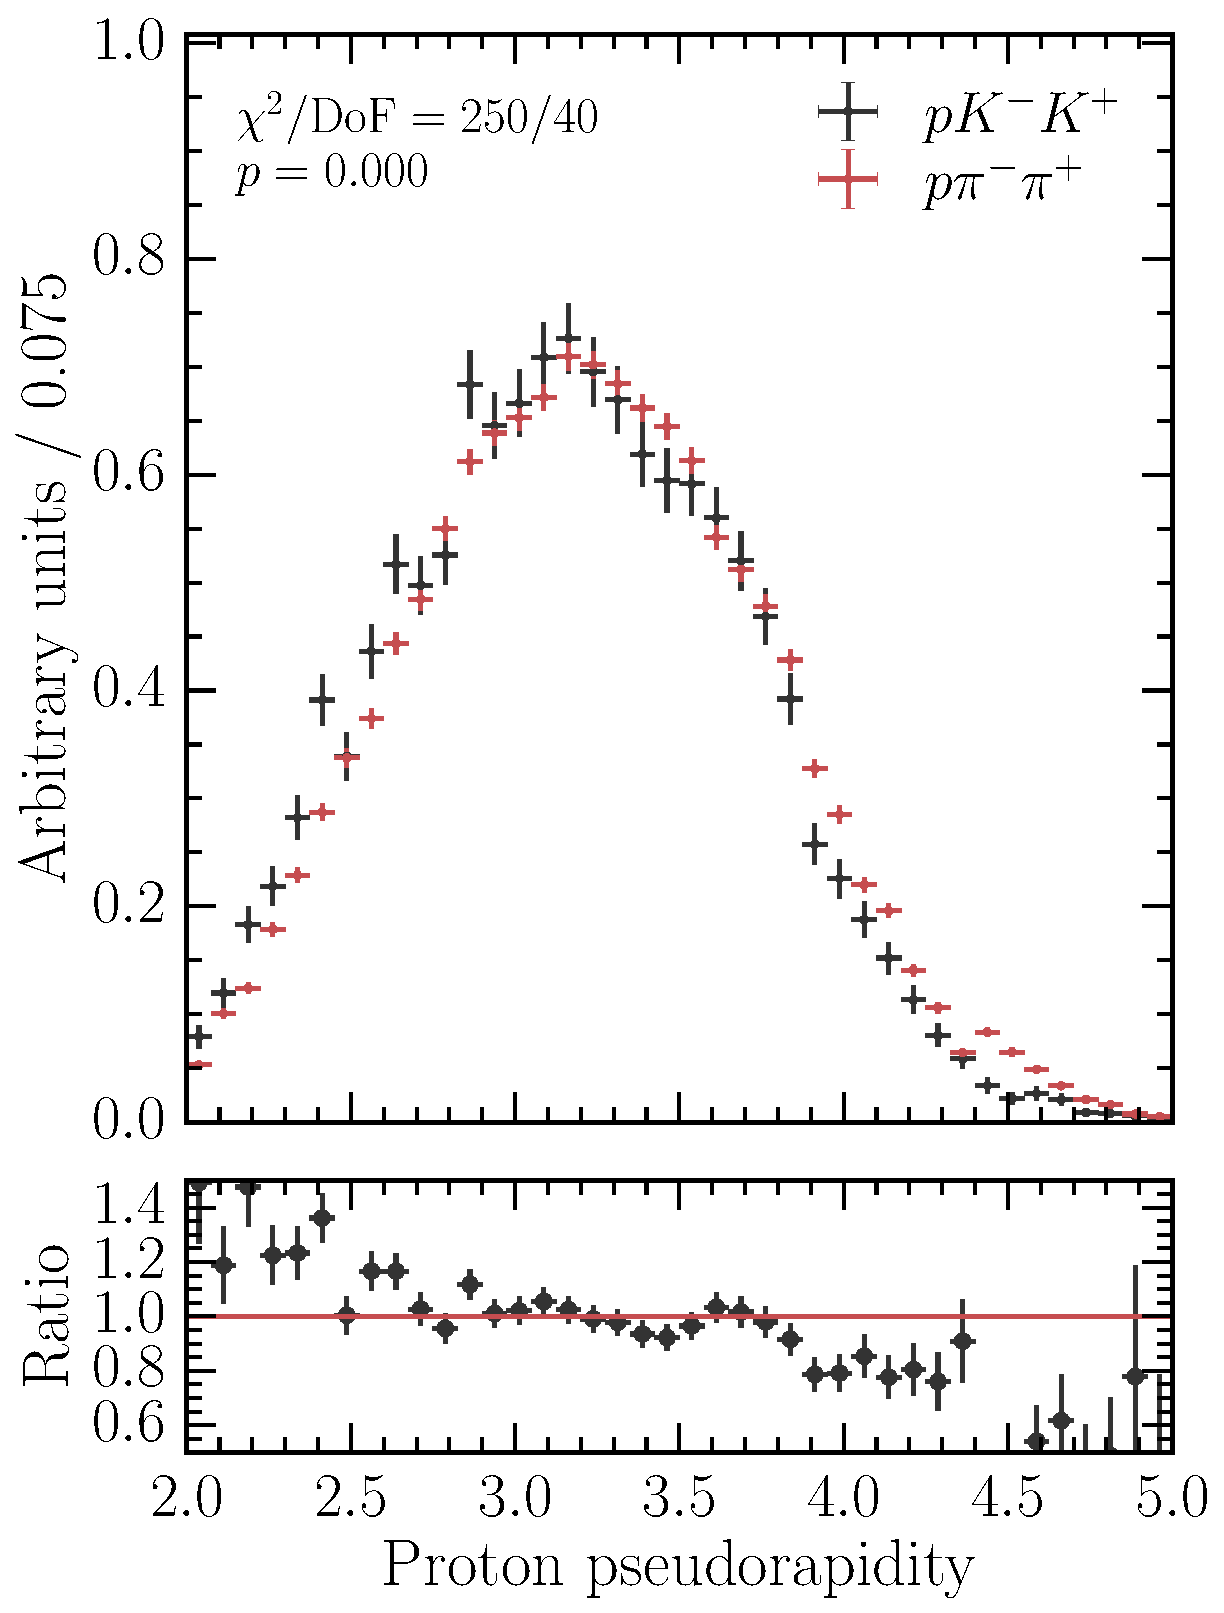
\includegraphics[width=\textwidth]{cpv/kinematic_weighting/preweighting_kinematics/LcToppipi_2012_MagDown_Lc_p_ETA}
    \label{fig:cpv:kinematic_weighting:pre:Lc_p:ETA}
  \end{subfigure}
  \begin{subfigure}[b]{0.4\textwidth}
    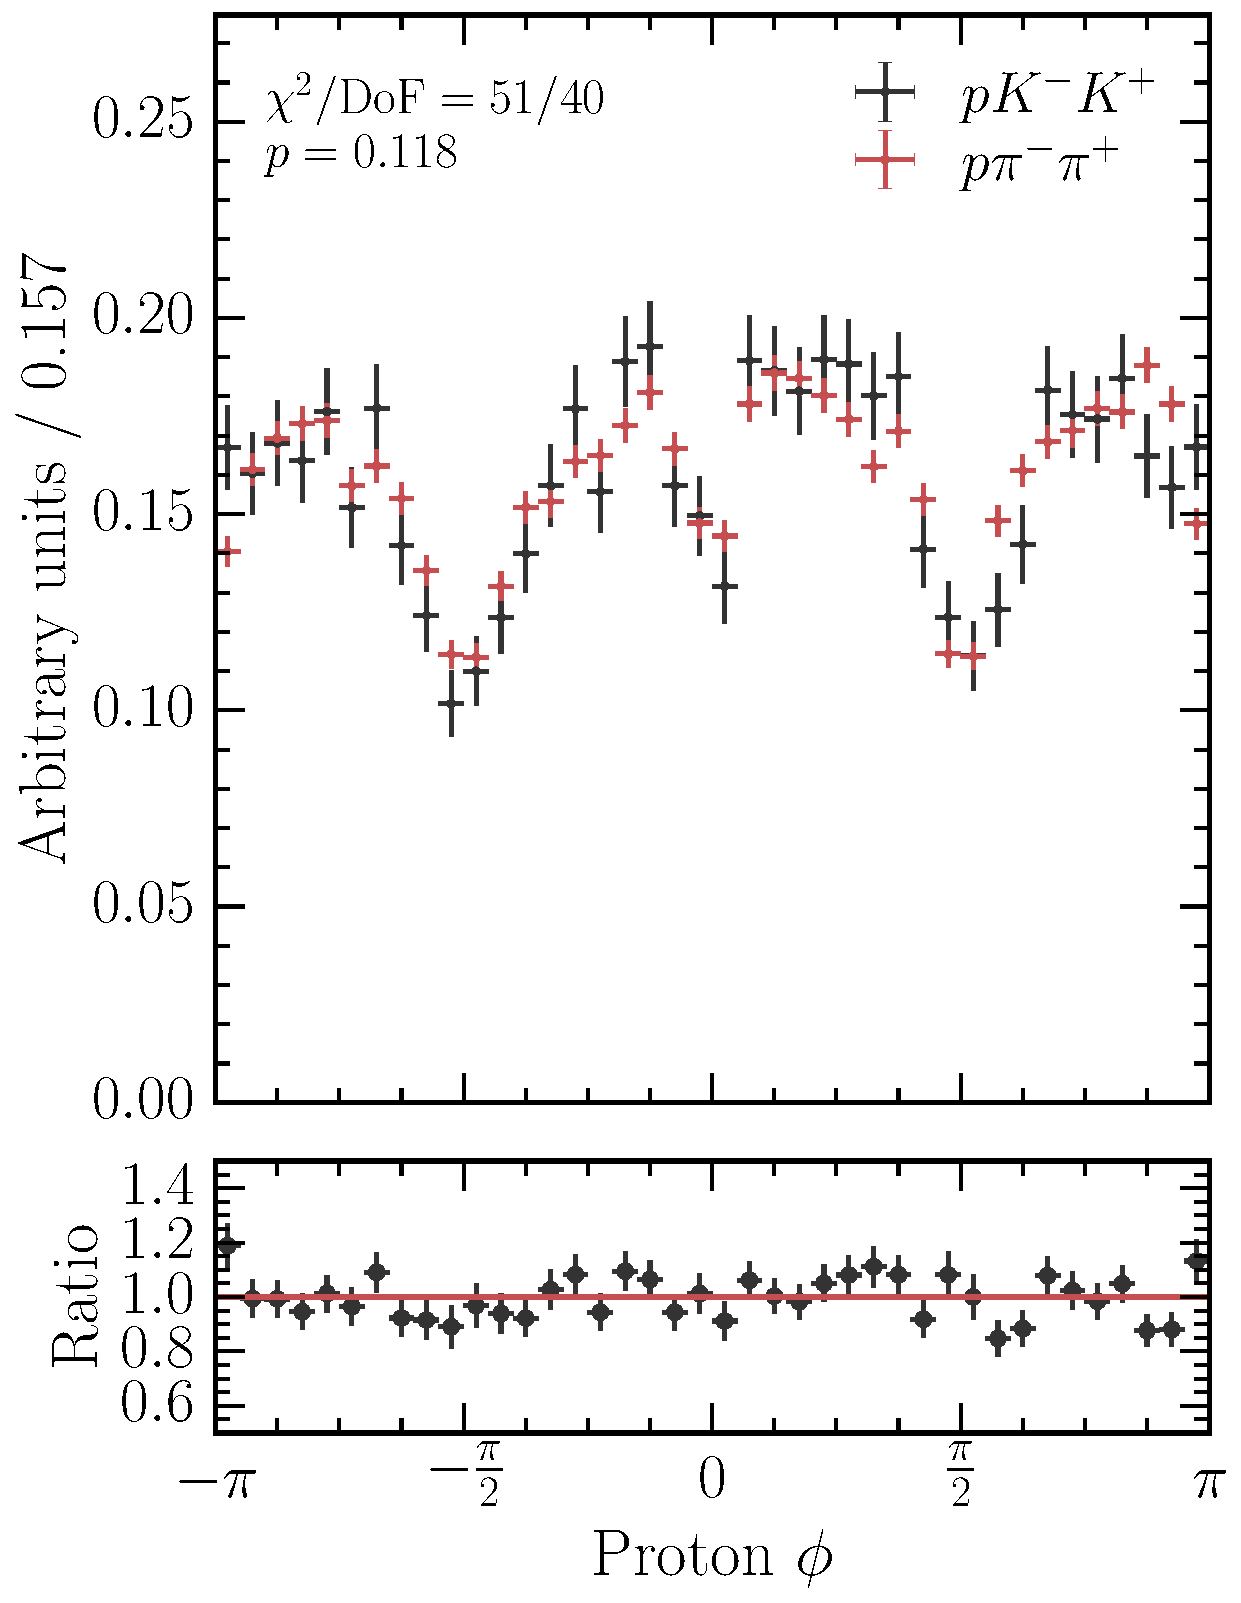
\includegraphics[width=\textwidth]{cpv/kinematic_weighting/preweighting_kinematics/LcToppipi_2012_MagDown_Lc_p_PHI}
    \label{fig:cpv:kinematic_weighting:pre:Lc_p:PHI}
  \end{subfigure}
  \caption{%
    Clockwise from the top left: total momentum, transverse momentum, angle 
    $\phi$, and pseudorapidity of the proton from the \PLambdac, weighted by 
    signal sWeights.
    The 2012 magnet down data is shown.
  }
  \label{fig:cpv:kinematic_weighting:pre:Lc_p}
\end{figure}

\begin{figure}
  \begin{subfigure}[b]{0.5\textwidth}
    \centering
    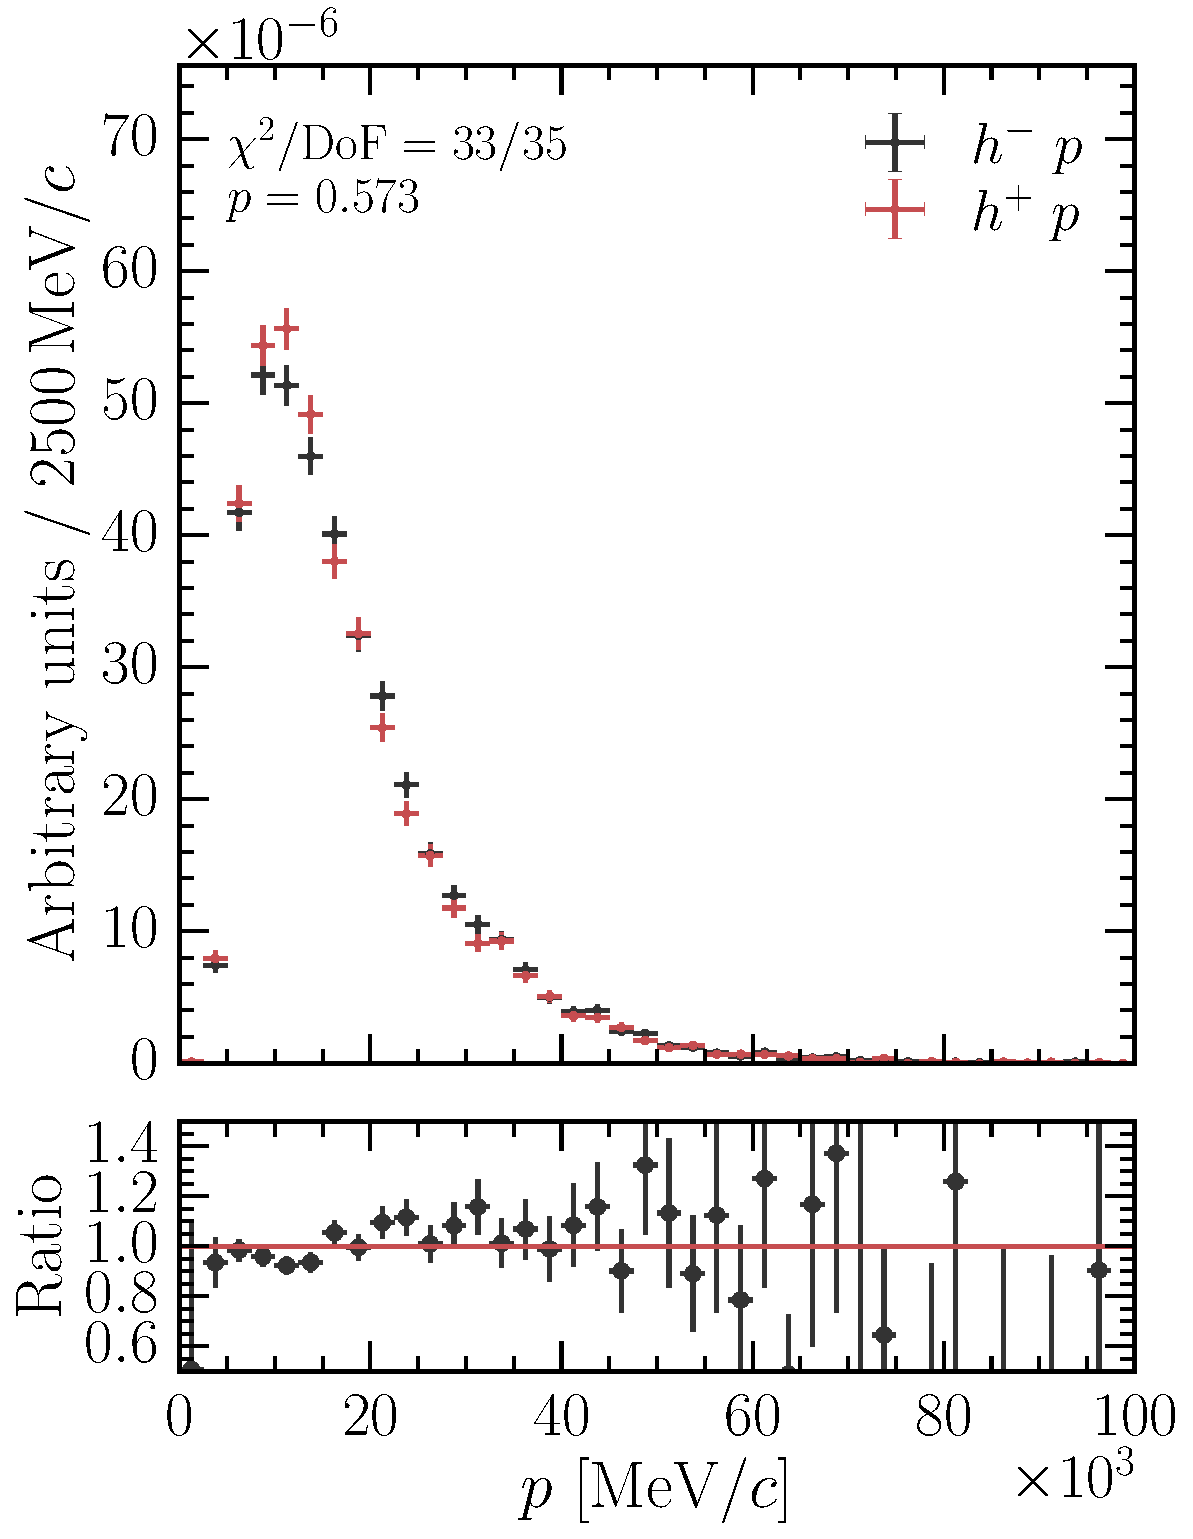
\includegraphics[width=0.8\textwidth]{cpv/kinematic_weighting/preweighting_kinematics/LcToppipi_2012_MagDown_h1_h2_P_LcTopKK}
    \label{fig:cpv:kinematic_weighting:pre:pKK_h1h2:P}
  \end{subfigure}
  \begin{subfigure}[b]{0.5\textwidth}
    \centering
    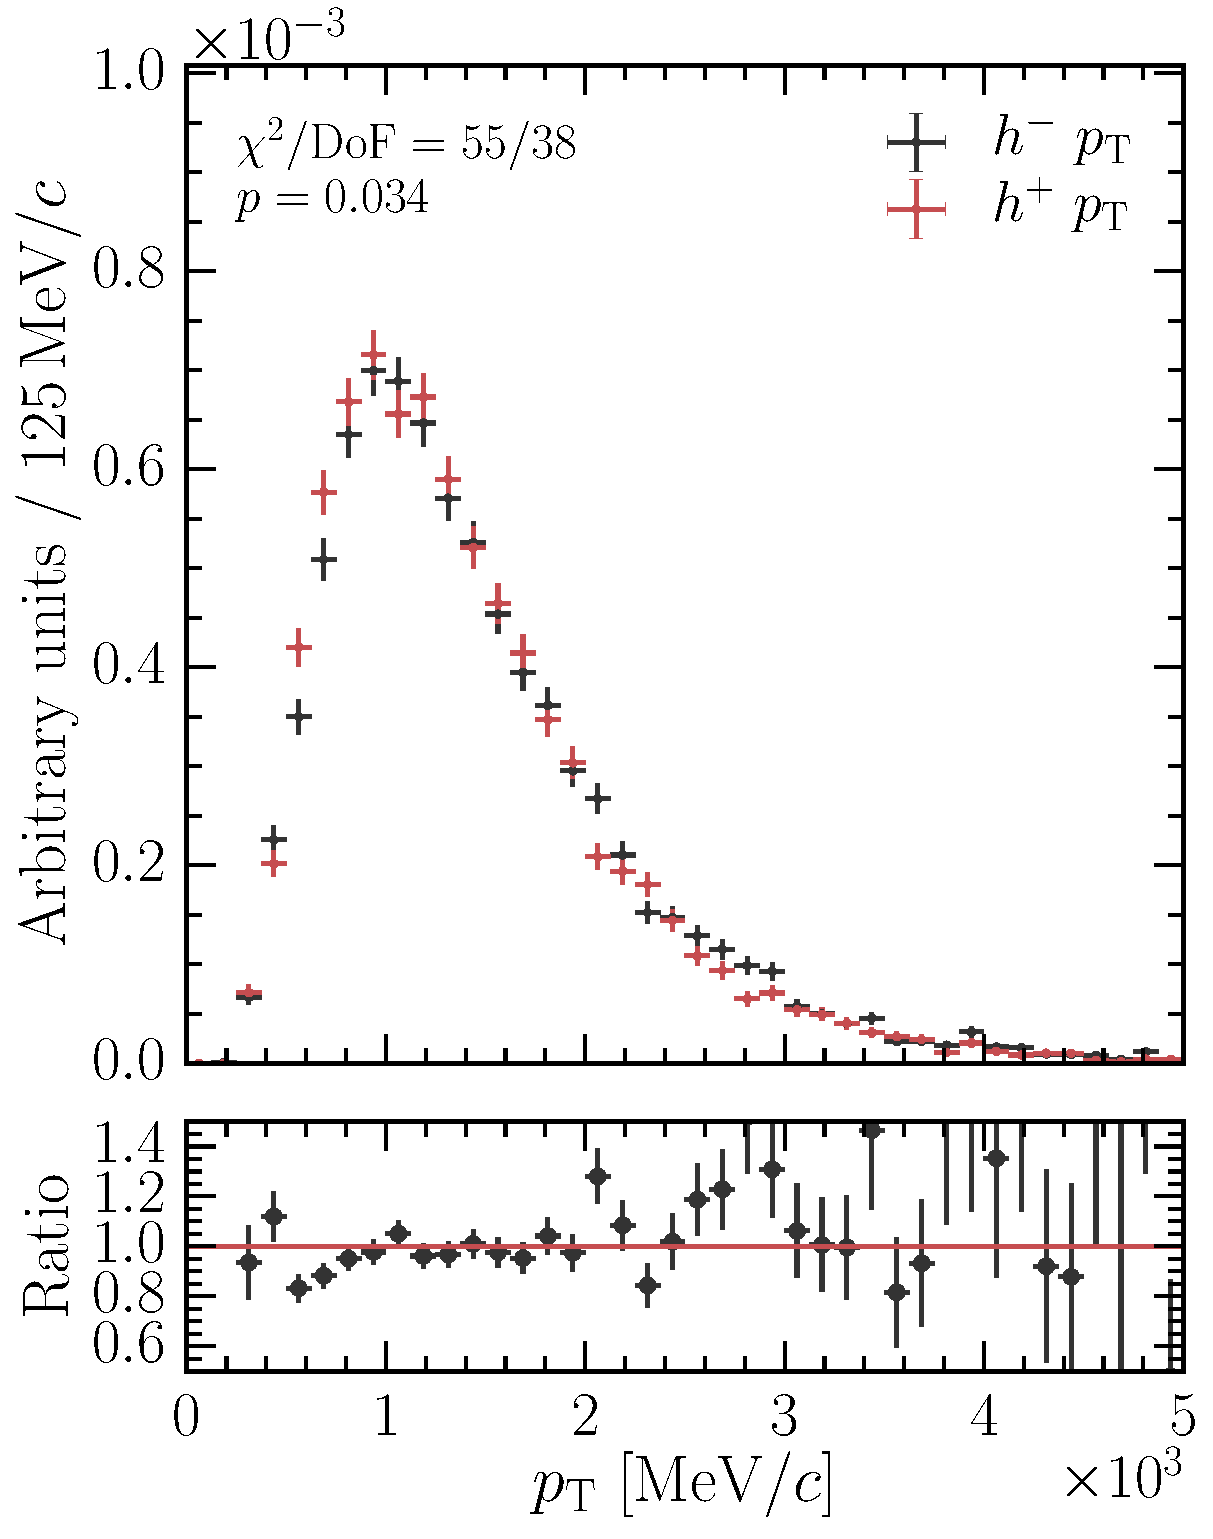
\includegraphics[width=0.8\textwidth]{cpv/kinematic_weighting/preweighting_kinematics/LcToppipi_2012_MagDown_h1_h2_PT_LcTopKK}
    \label{fig:cpv:kinematic_weighting:pre:pKK_h1h2:PT}
  \end{subfigure}\\
  \begin{subfigure}[b]{\textwidth}
    \centering
    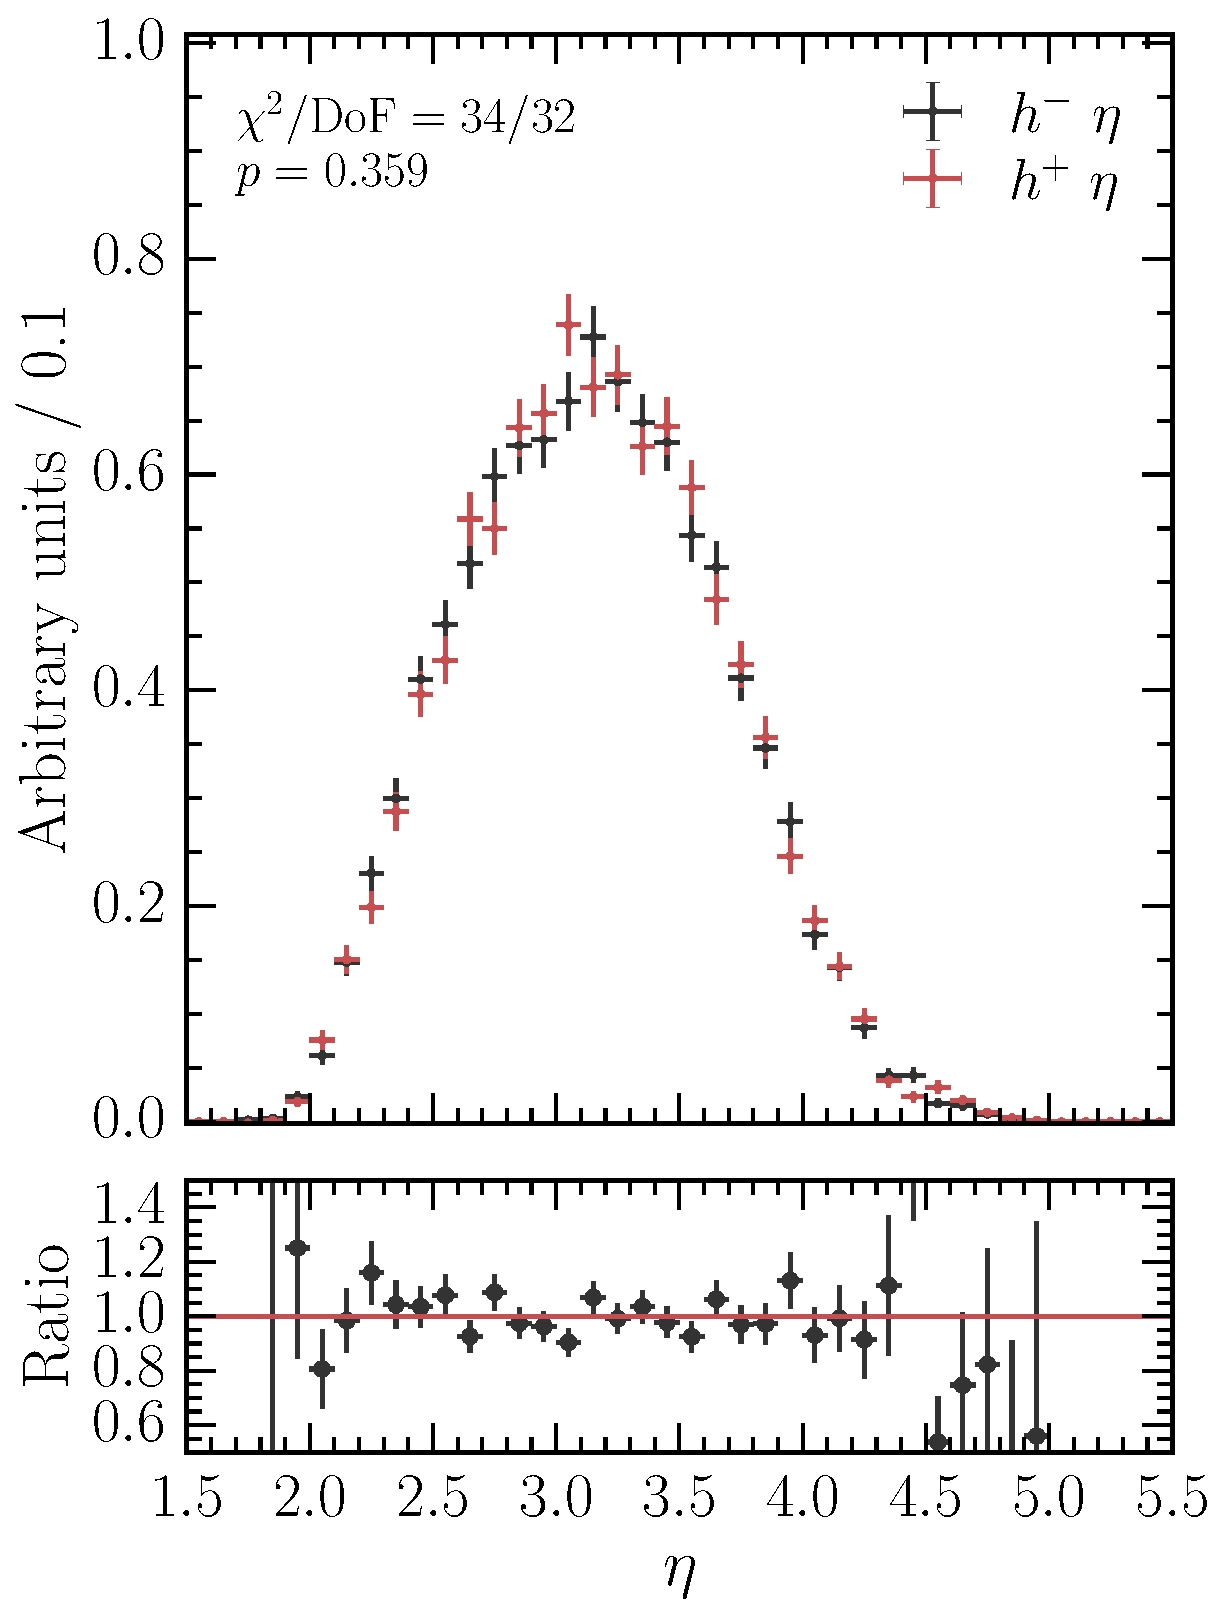
\includegraphics[width=0.4\textwidth]{cpv/kinematic_weighting/preweighting_kinematics/LcToppipi_2012_MagDown_h1_h2_ETA_LcTopKK}
    \label{fig:cpv:kinematic_weighting:pre:pKK_h1h2:ETA}
  \end{subfigure}
  \caption{%
    Clockwise from the top left: total momentum, transverse momentum, and 
    pseudorapidity of the \PKminus\ and \PKplus\ \PLambdac\ children in the 
    \pKK\ data, weighted by signal sWeights.
    The 2012 magnet down data is shown.
  }
  \label{fig:cpv:kinematic_weighting:pre:pKK_h1h2}
\end{figure}

\begin{figure}
  \begin{subfigure}[b]{0.5\textwidth}
    \centering
    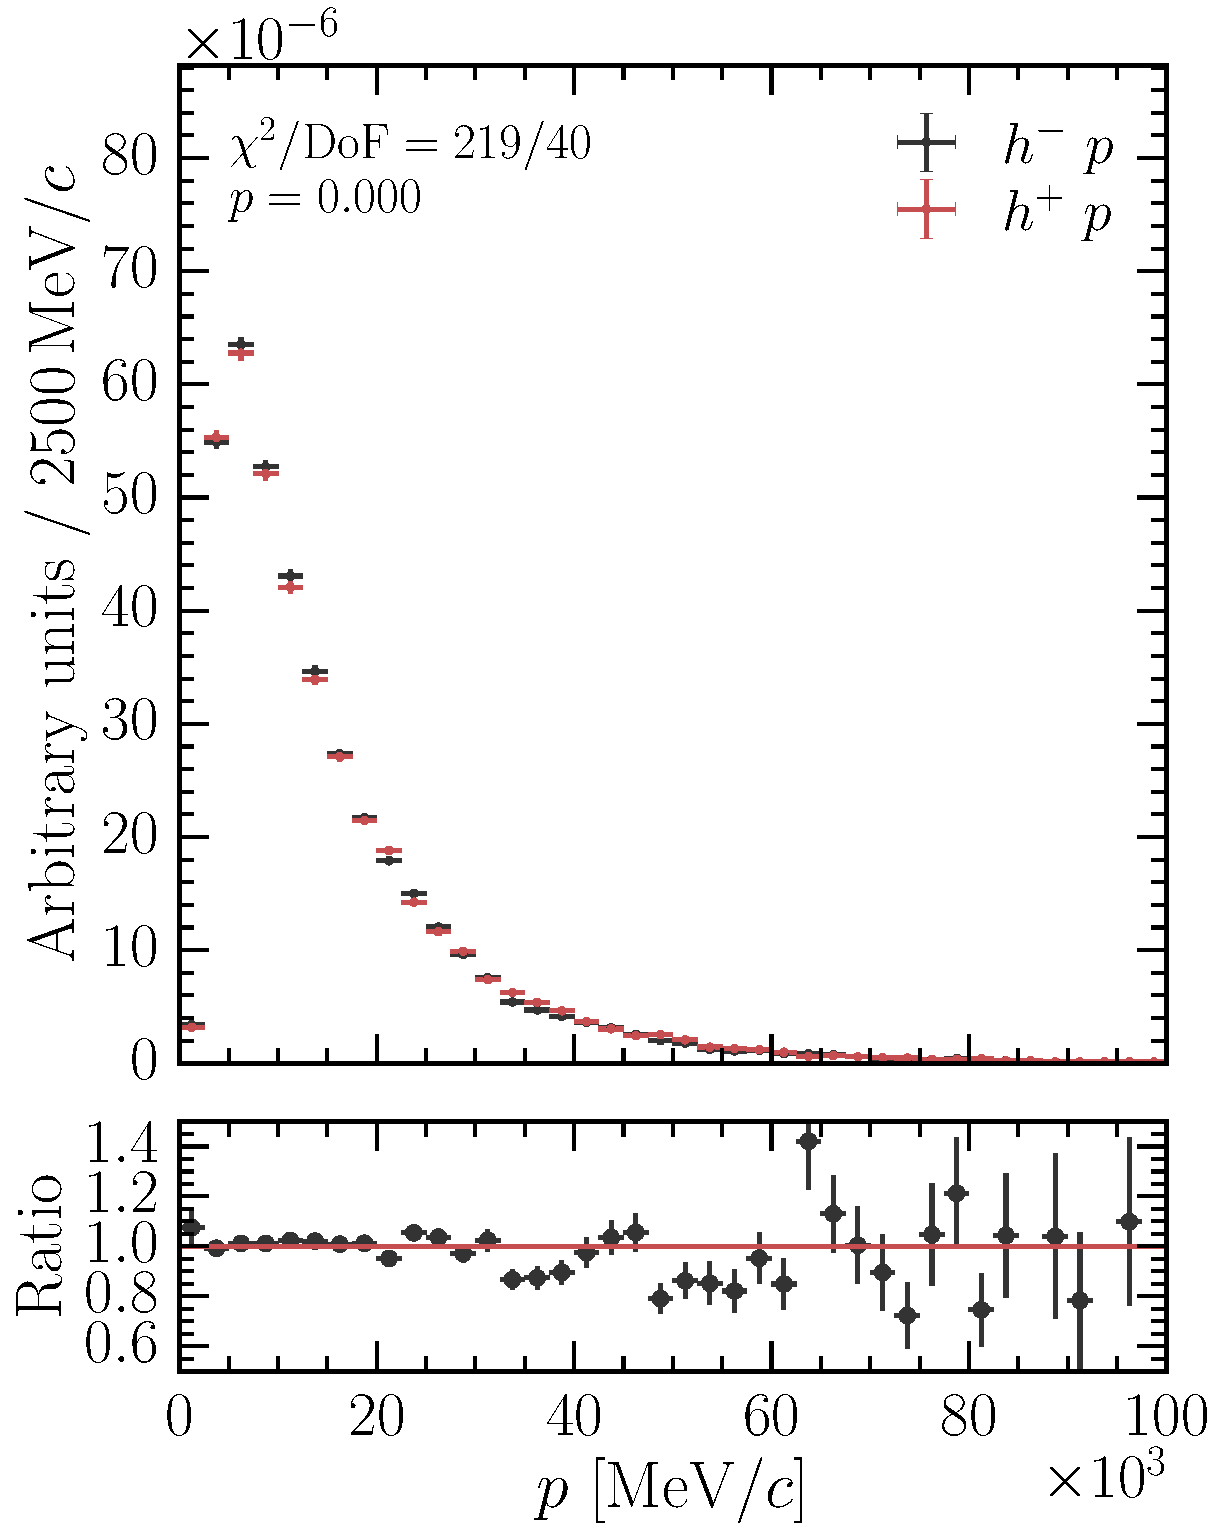
\includegraphics[width=0.8\textwidth]{cpv/kinematic_weighting/preweighting_kinematics/LcToppipi_2012_MagDown_h1_h2_P_LcToppipi}
    \label{fig:cpv:kinematic_weighting:pre:ppipi_h1h2:P}
  \end{subfigure}
  \begin{subfigure}[b]{0.5\textwidth}
    \centering
    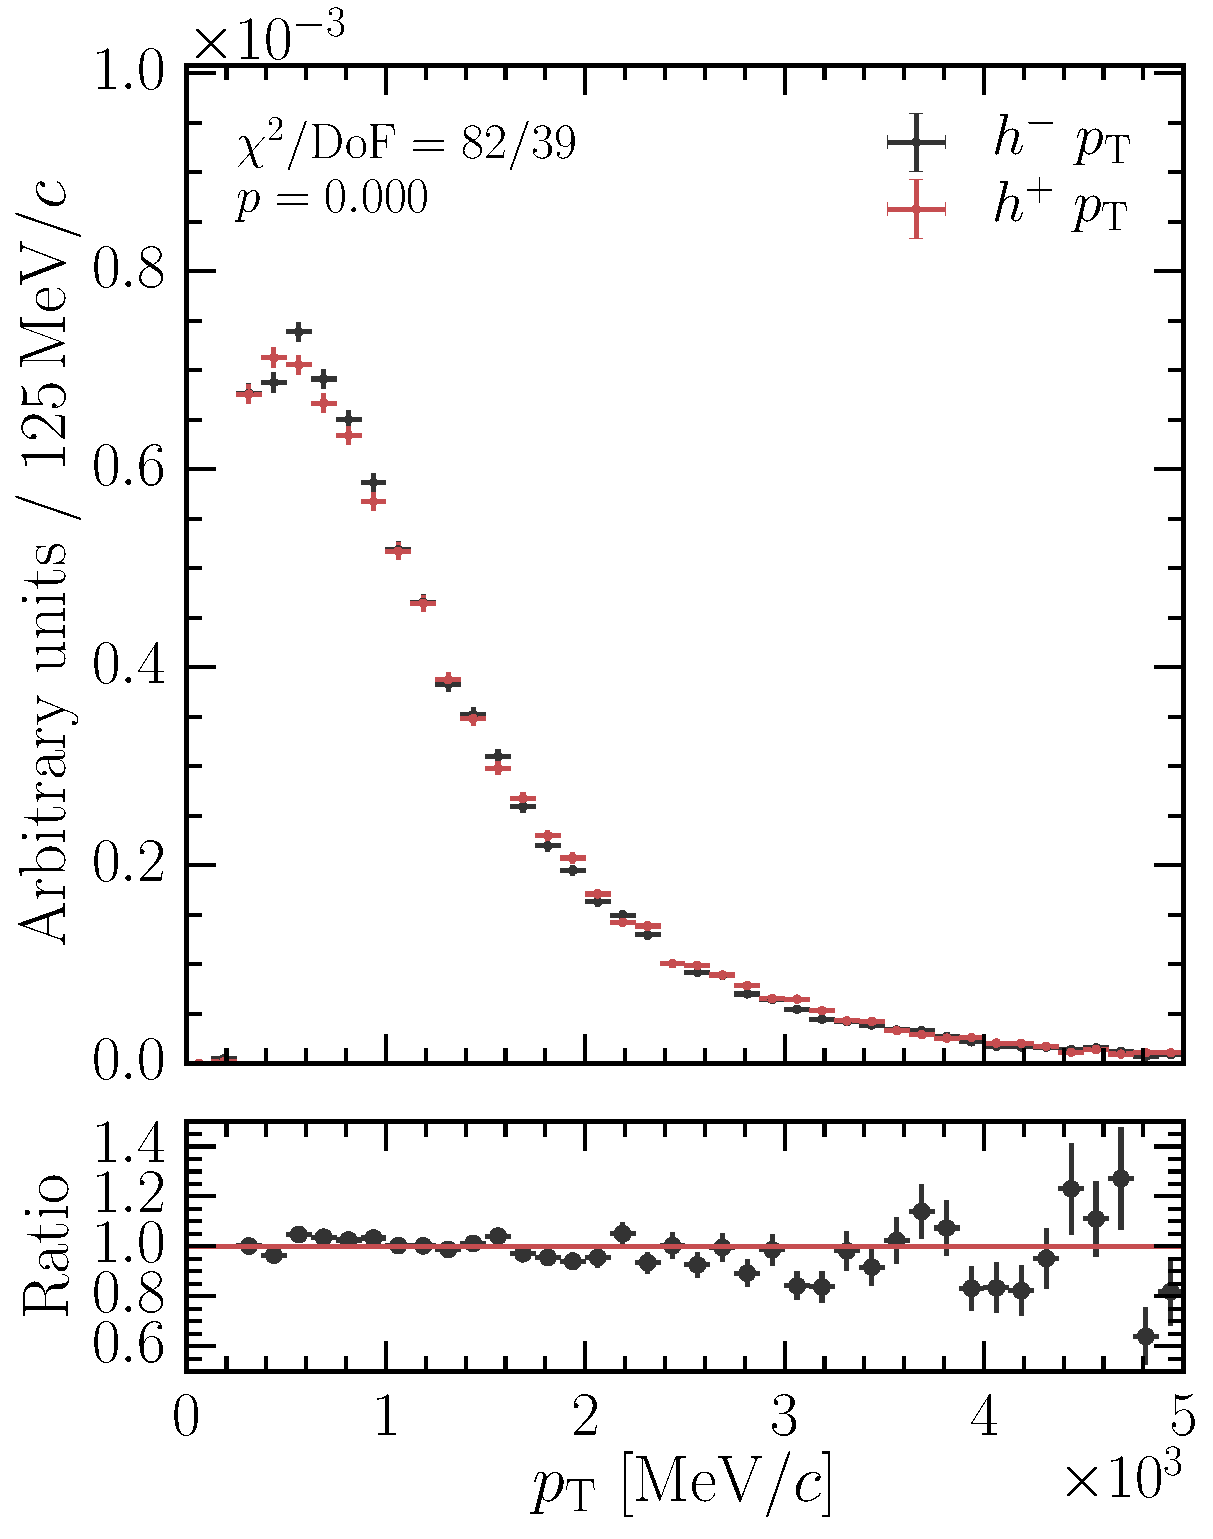
\includegraphics[width=0.8\textwidth]{cpv/kinematic_weighting/preweighting_kinematics/LcToppipi_2012_MagDown_h1_h2_PT_LcToppipi}
    \label{fig:cpv:kinematic_weighting:pre:ppipi_h1h2:PT}
  \end{subfigure}\\
  \begin{subfigure}[b]{\textwidth}
    \centering
    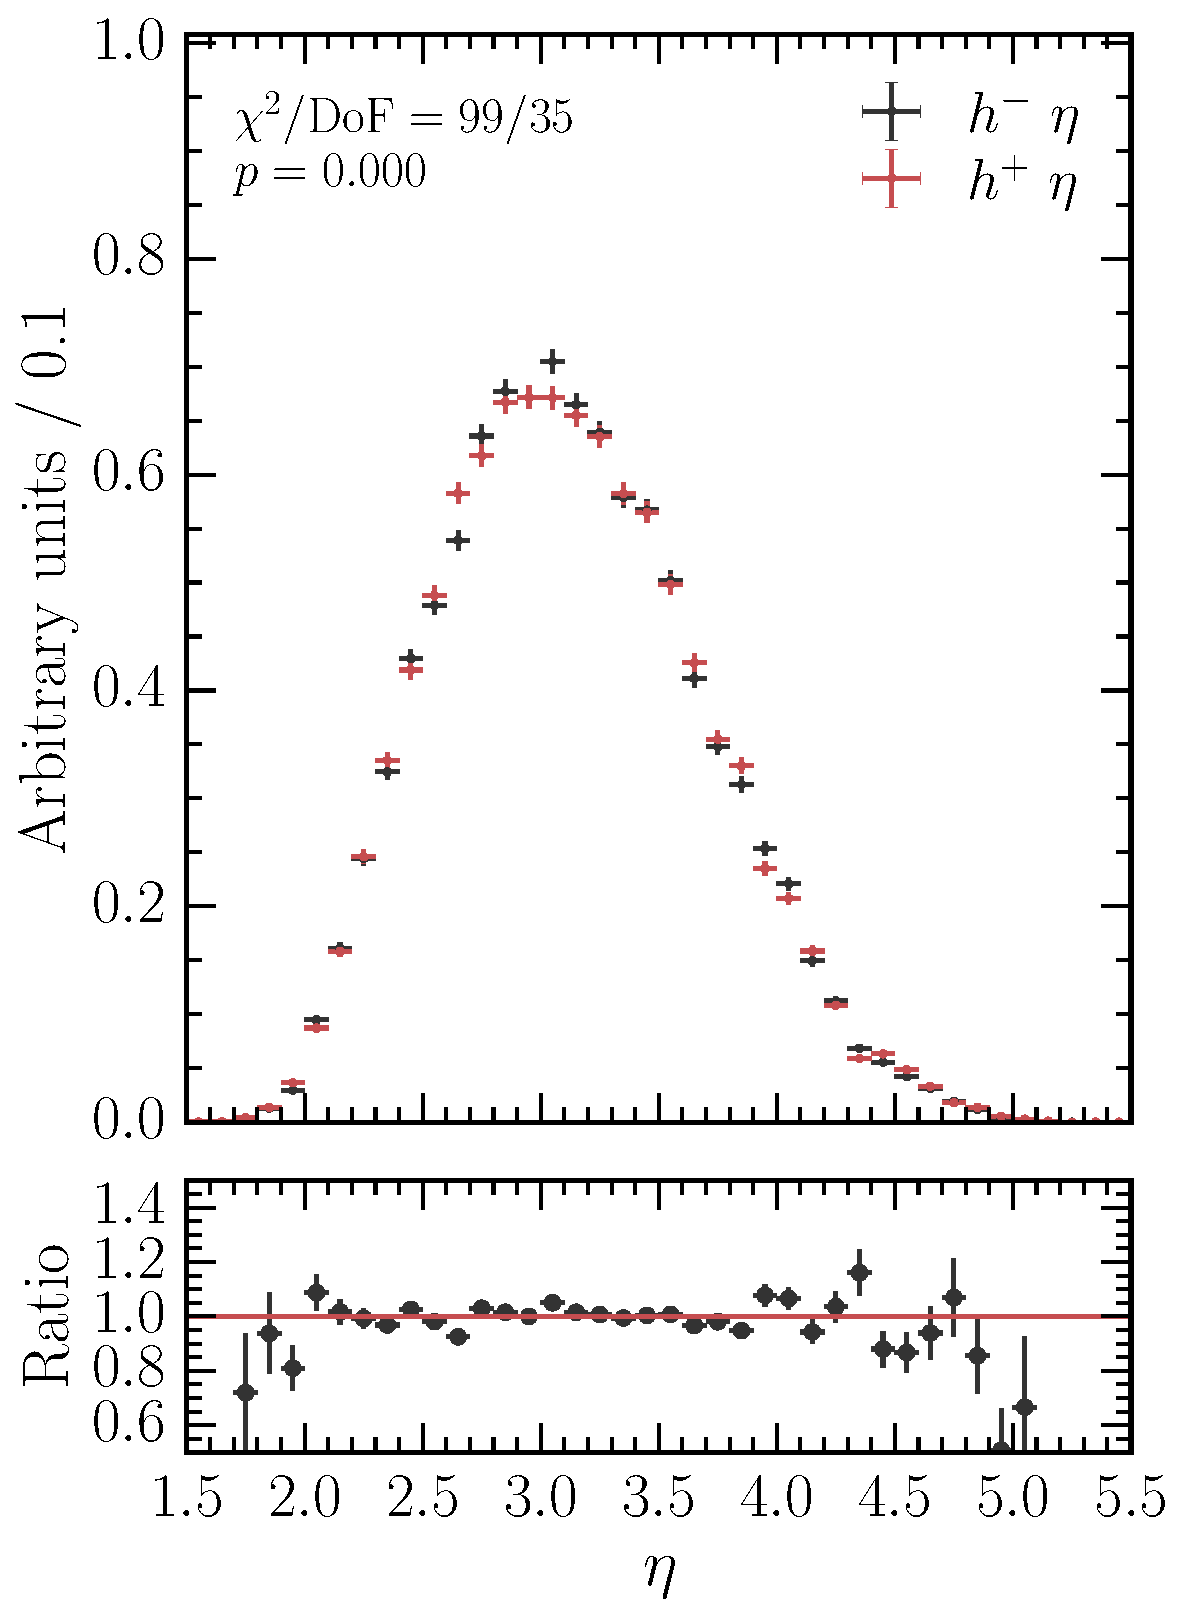
\includegraphics[width=0.4\textwidth]{cpv/kinematic_weighting/preweighting_kinematics/LcToppipi_2012_MagDown_h1_h2_ETA_LcToppipi}
    \label{fig:cpv:kinematic_weighting:pre:ppipi_h1h2:ETA}
  \end{subfigure}
  \caption{%
    Clockwise from the top left: total momentum, transverse momentum, and 
    pseudorapidity of the \Ppiminus\ and \Ppiplus\ \PLambdac\ children in the 
    \ppipi\ data, weighted by signal sWeights.
    The 2012 magnet down data is shown.
  }
  \label{fig:cpv:kinematic_weighting:pre:ppipi_h1h2}
\end{figure}

\begin{figure}
  \begin{subfigure}[b]{0.4\textwidth}
    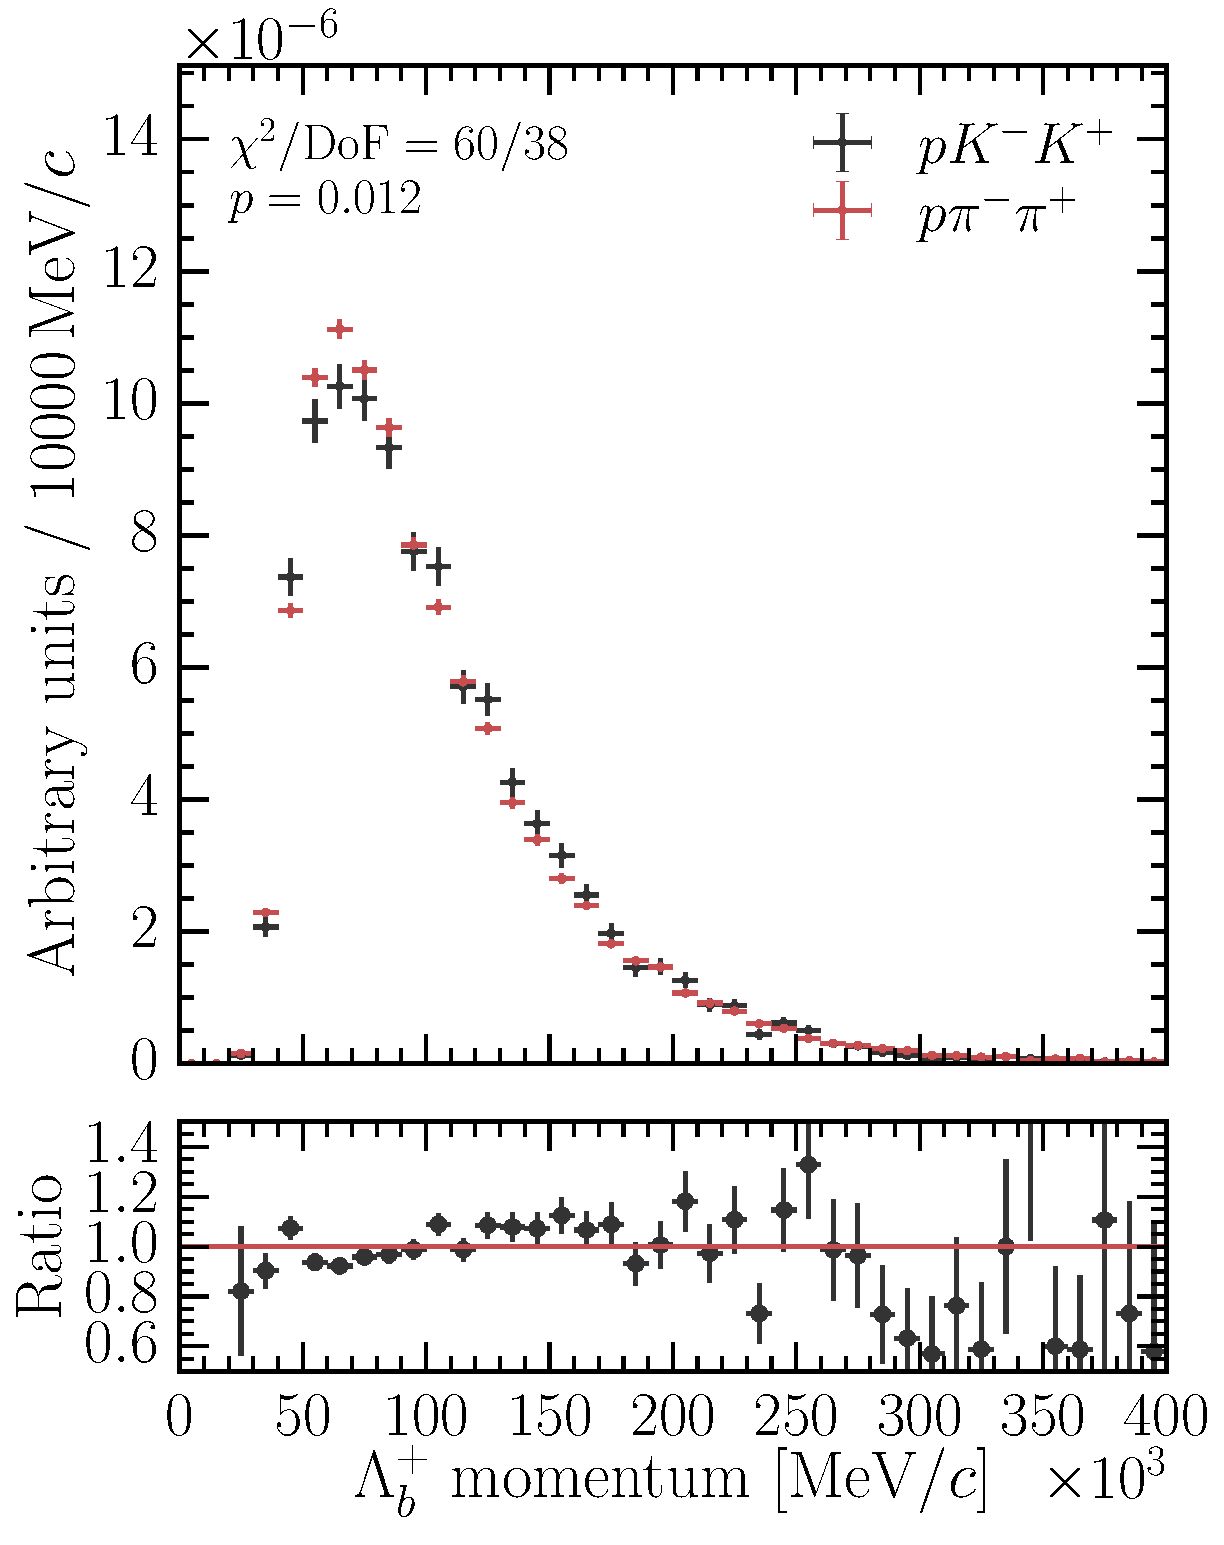
\includegraphics[width=\textwidth]{cpv/kinematic_weighting/postweighting_kinematics/LcToppipi_2012_MagDown_Lb_P-weighted}
    \label{fig:cpv:kinematic_weighting:post:Lb:P}
  \end{subfigure}
  \begin{subfigure}[b]{0.4\textwidth}
    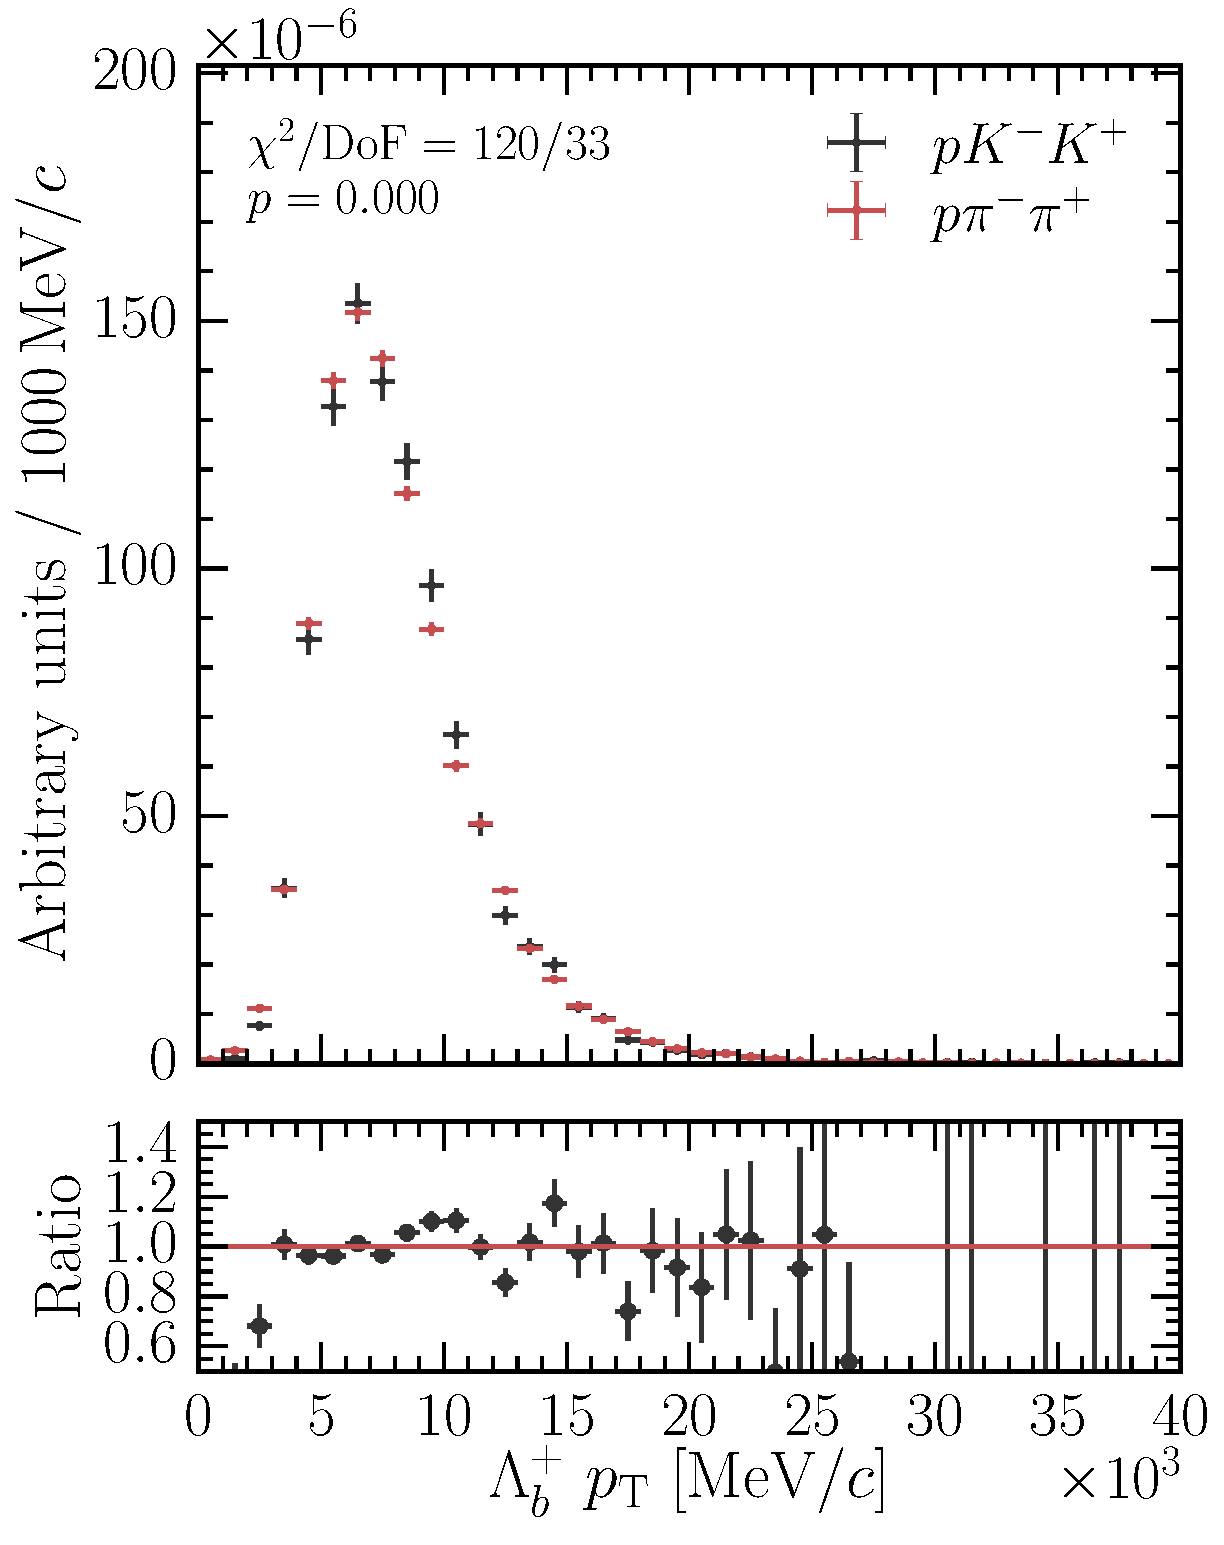
\includegraphics[width=\textwidth]{cpv/kinematic_weighting/postweighting_kinematics/LcToppipi_2012_MagDown_Lb_PT-weighted}
    \label{fig:cpv:kinematic_weighting:post:Lb:PT}
  \end{subfigure}\\
  \begin{subfigure}[b]{0.4\textwidth}
    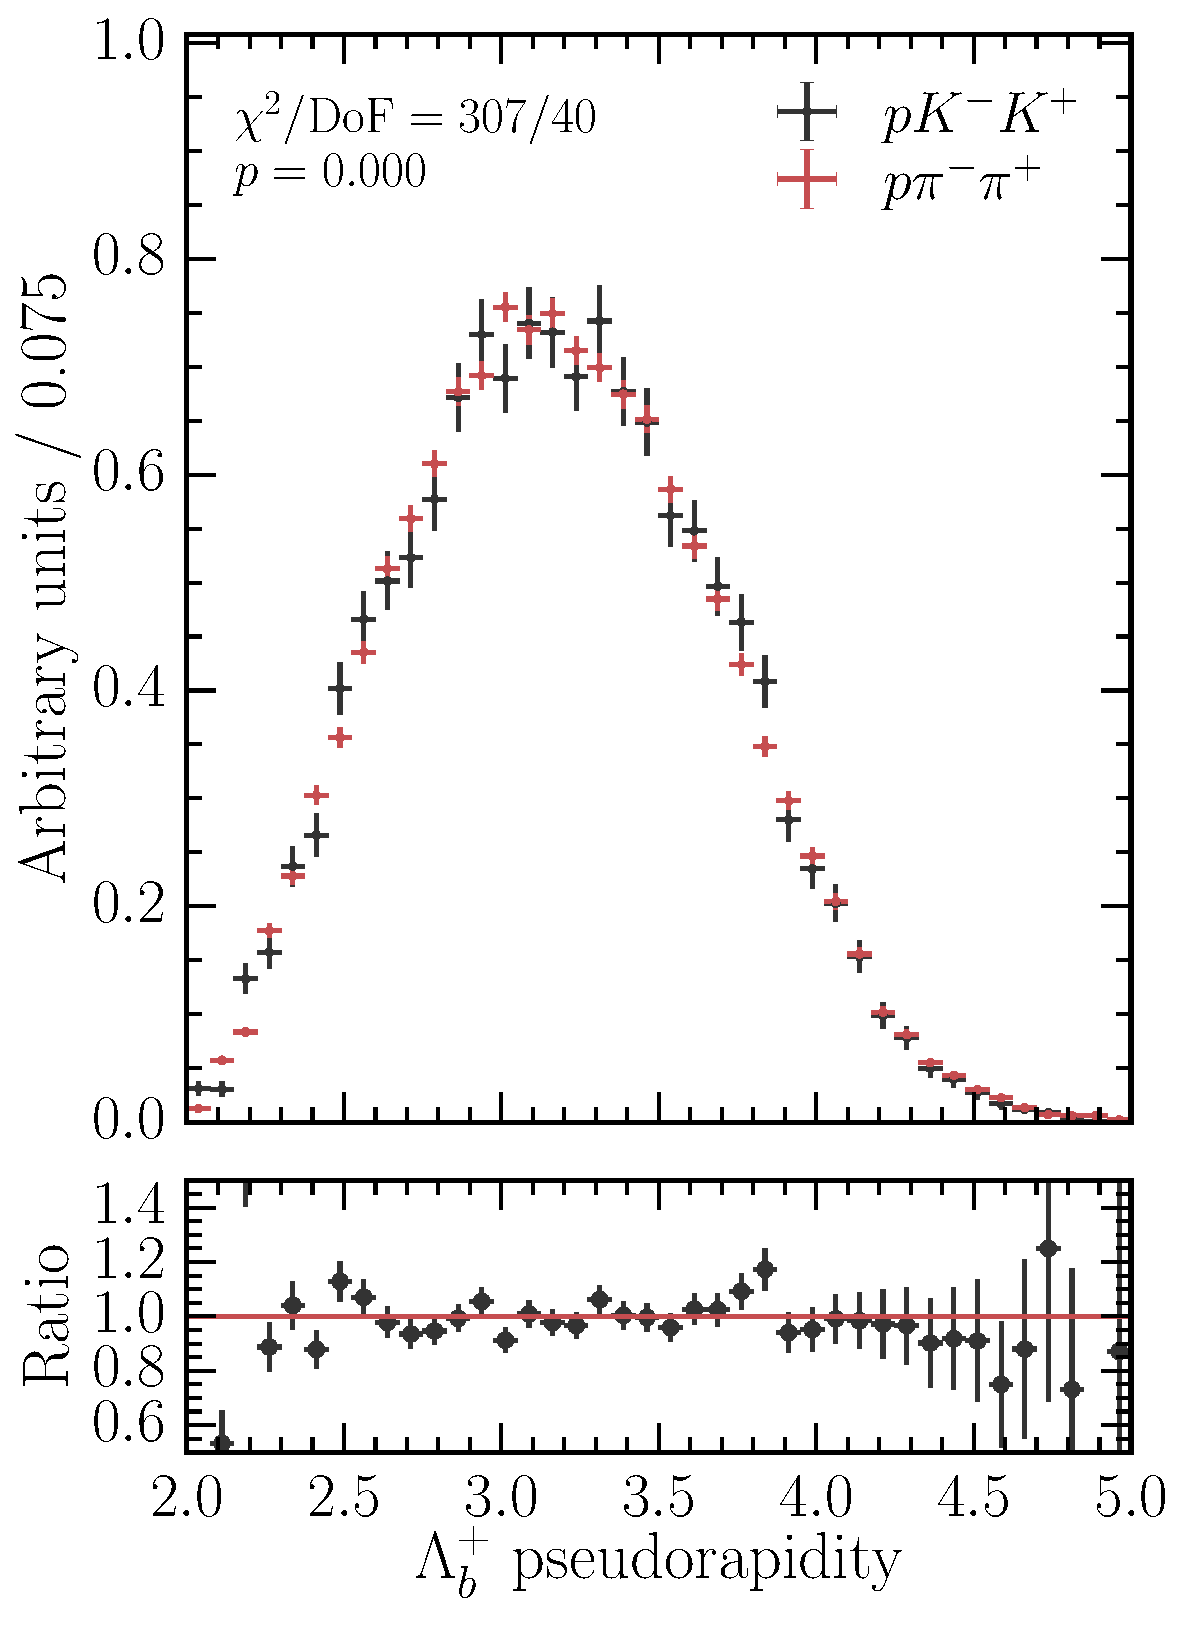
\includegraphics[width=\textwidth]{cpv/kinematic_weighting/postweighting_kinematics/LcToppipi_2012_MagDown_Lb_ETA-weighted}
    \label{fig:cpv:kinematic_weighting:post:Lb:ETA}
  \end{subfigure}
  \begin{subfigure}[b]{0.4\textwidth}
    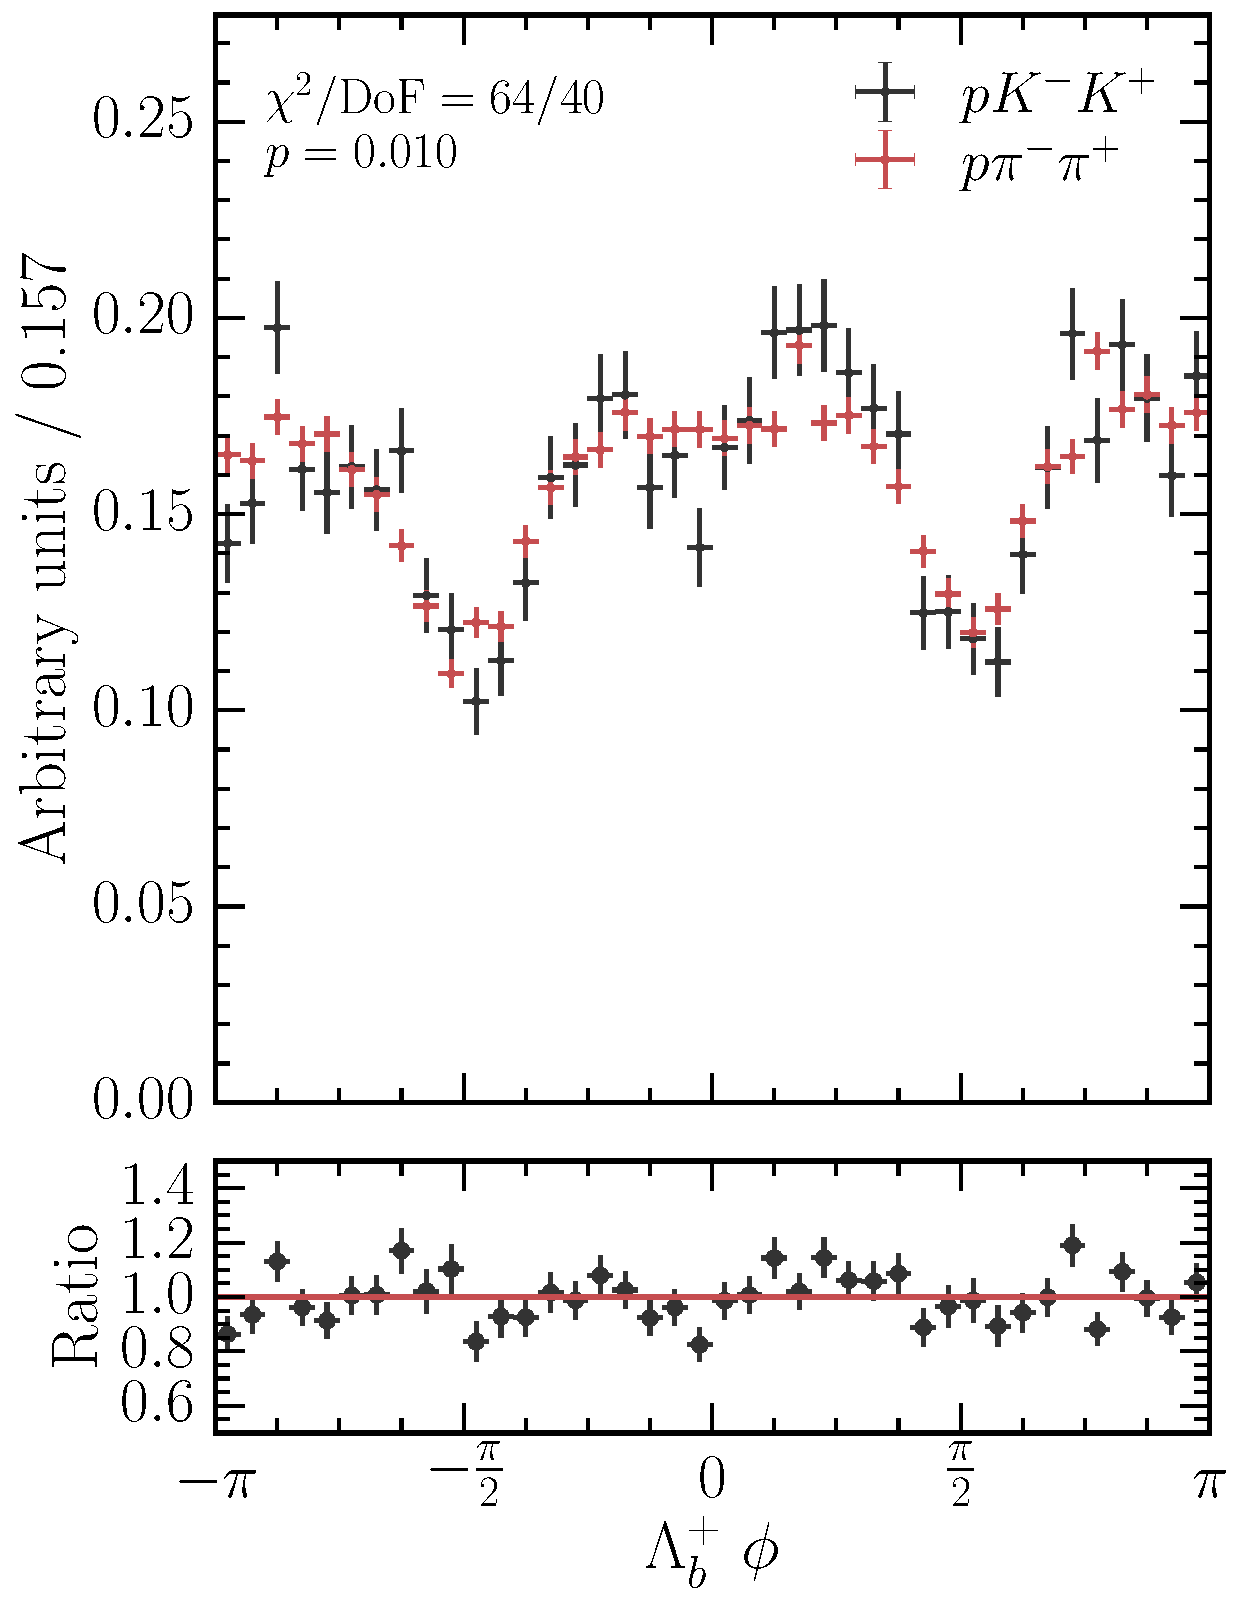
\includegraphics[width=\textwidth]{cpv/kinematic_weighting/postweighting_kinematics/LcToppipi_2012_MagDown_Lb_PHI-weighted}
    \label{fig:cpv:kinematic_weighting:post:Lb:PHI}
  \end{subfigure}
  \caption{%
    Clockwise from the top left: total momentum, transverse momentum, angle 
    $\phi$, and pseudorapidity of the \PLambdab, weighted by the product of 
    signal sWeights and kinematic weights.
    The 2012 magnet down data is shown.
  }
  \label{fig:cpv:kinematic_weighting:post:Lb}
\end{figure}

\begin{figure}
  \begin{subfigure}[b]{0.4\textwidth}
    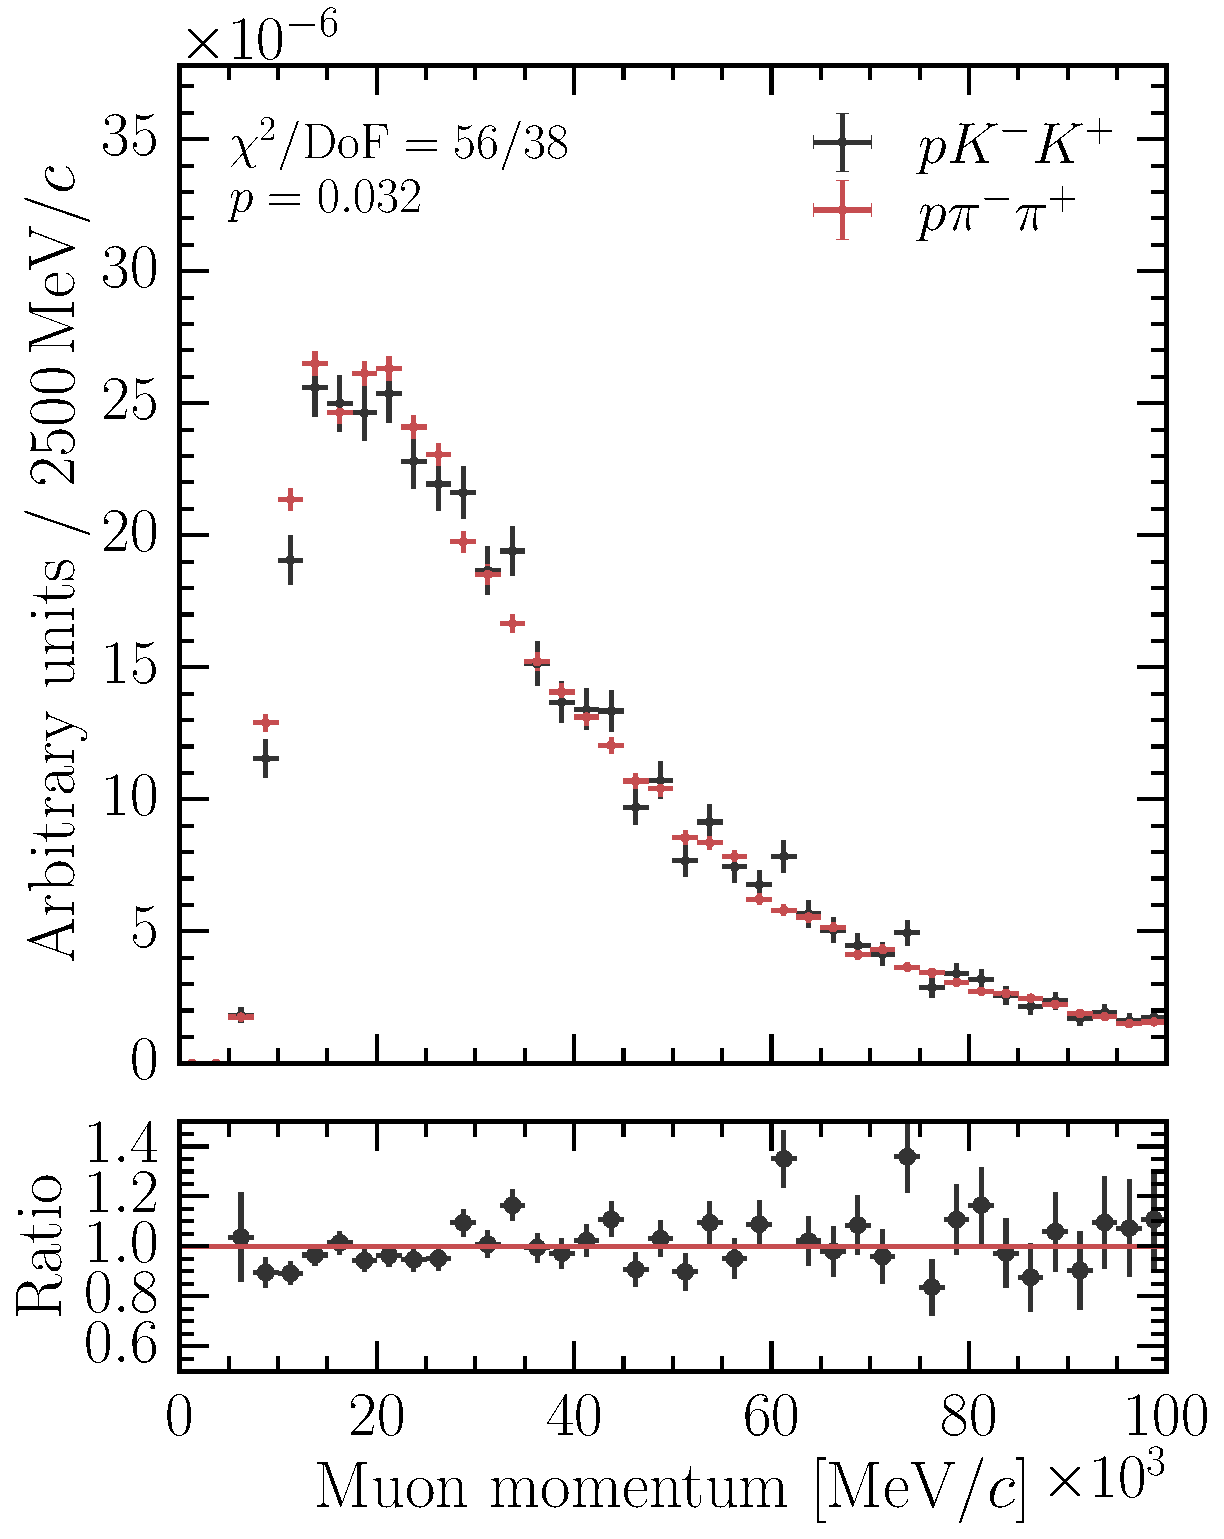
\includegraphics[width=\textwidth]{cpv/kinematic_weighting/postweighting_kinematics/LcToppipi_2012_MagDown_Lb_mu_P-weighted}
    \label{fig:cpv:kinematic_weighting:post:Lb_mu:P}
  \end{subfigure}
  \begin{subfigure}[b]{0.4\textwidth}
    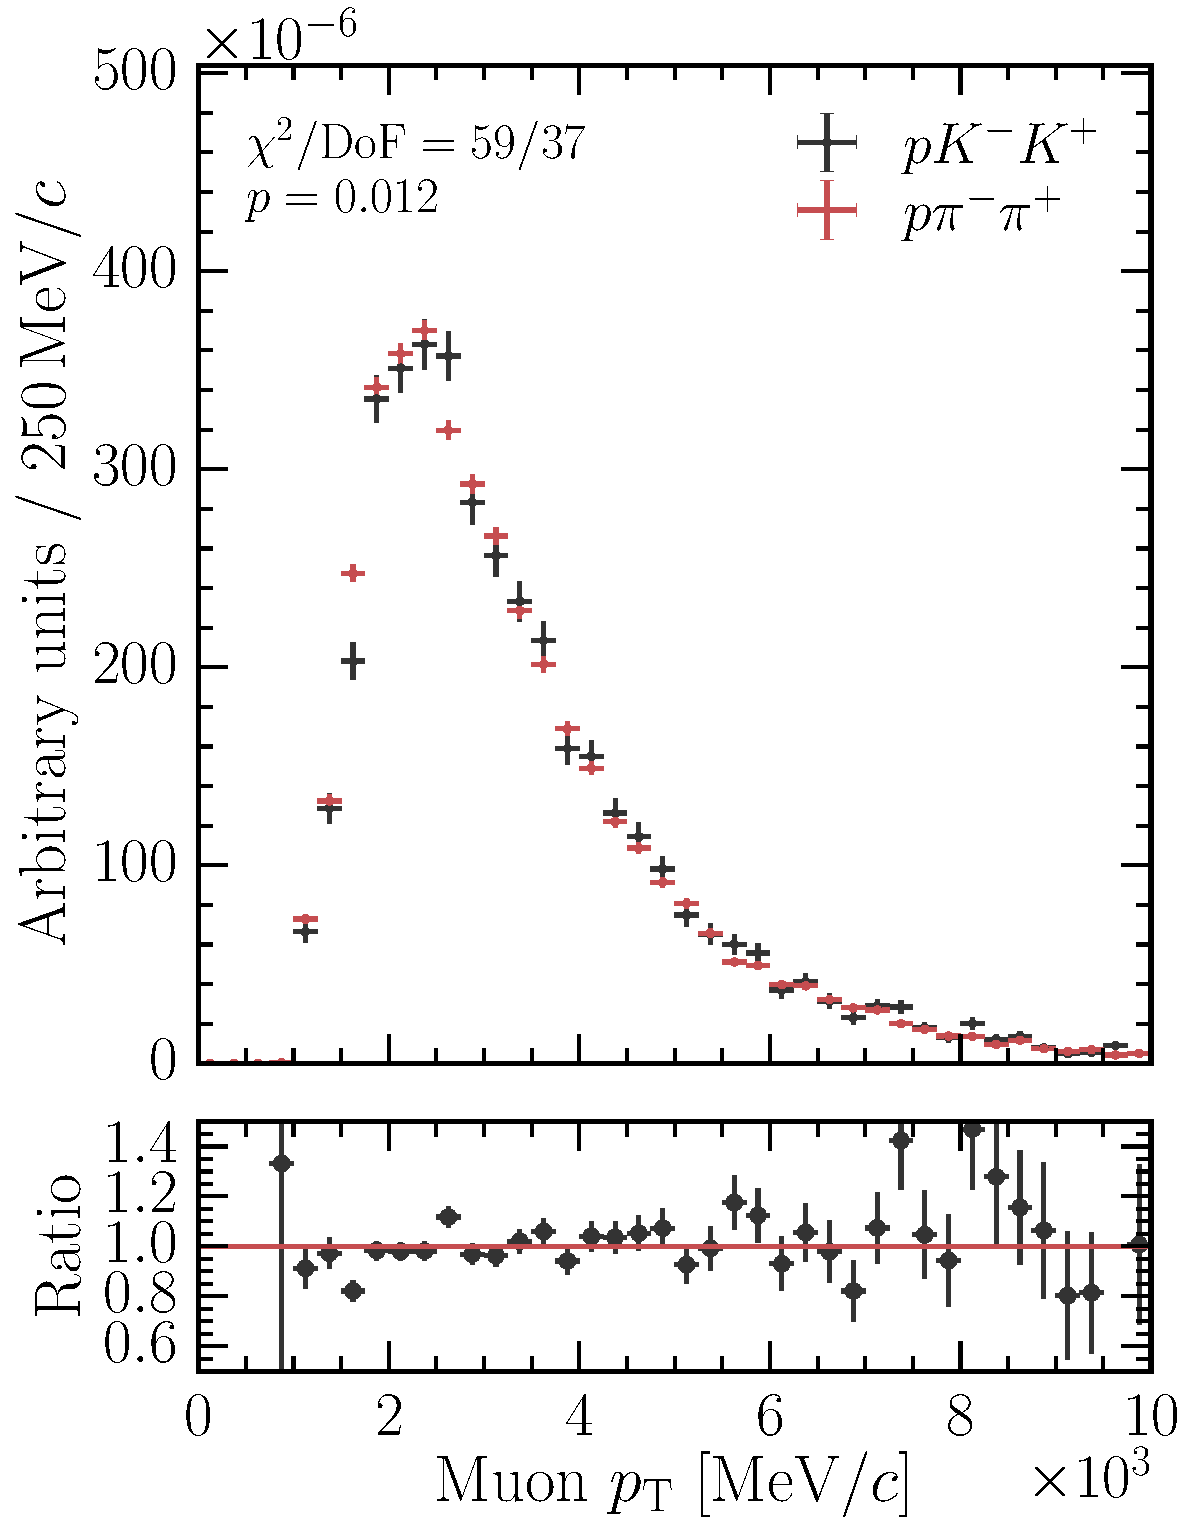
\includegraphics[width=\textwidth]{cpv/kinematic_weighting/postweighting_kinematics/LcToppipi_2012_MagDown_Lb_mu_PT-weighted}
    \label{fig:cpv:kinematic_weighting:post:Lb_mu:PT}
  \end{subfigure}\\
  \begin{subfigure}[b]{0.4\textwidth}
    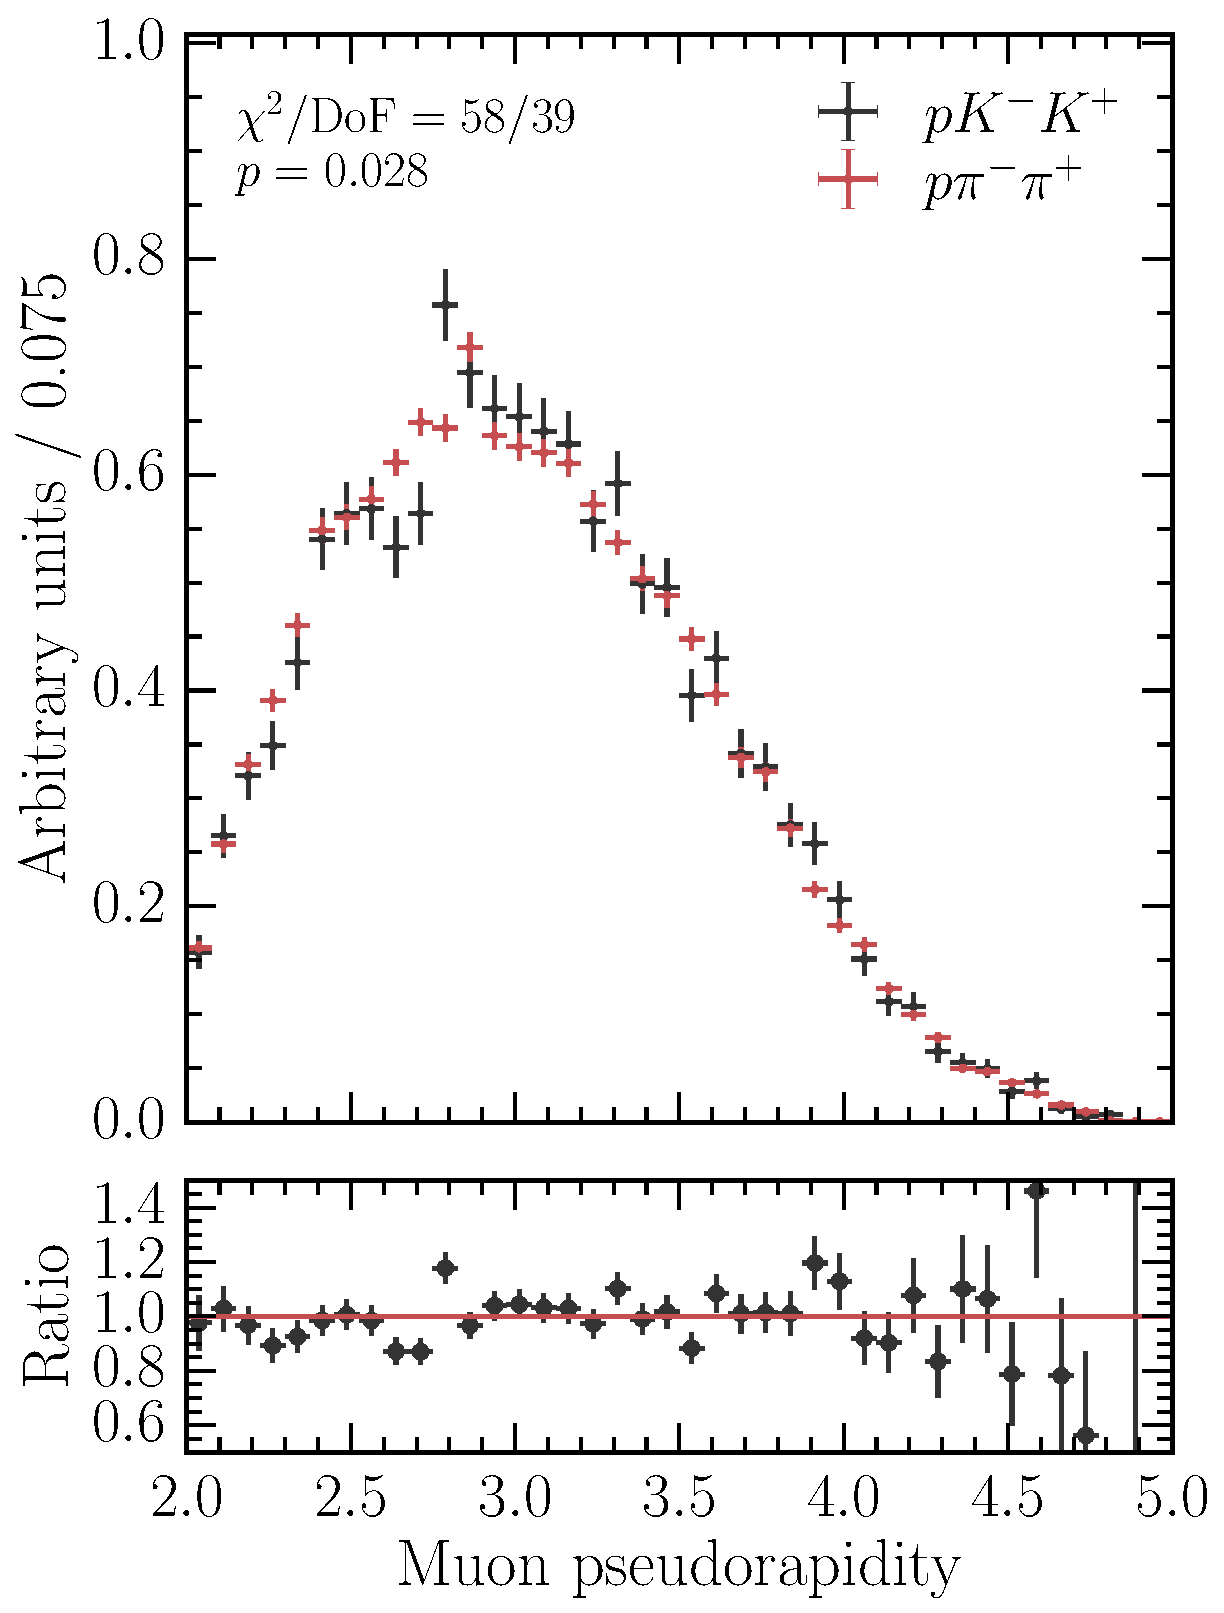
\includegraphics[width=\textwidth]{cpv/kinematic_weighting/postweighting_kinematics/LcToppipi_2012_MagDown_Lb_mu_ETA-weighted}
    \label{fig:cpv:kinematic_weighting:post:Lb_mu:ETA}
  \end{subfigure}
  \begin{subfigure}[b]{0.4\textwidth}
    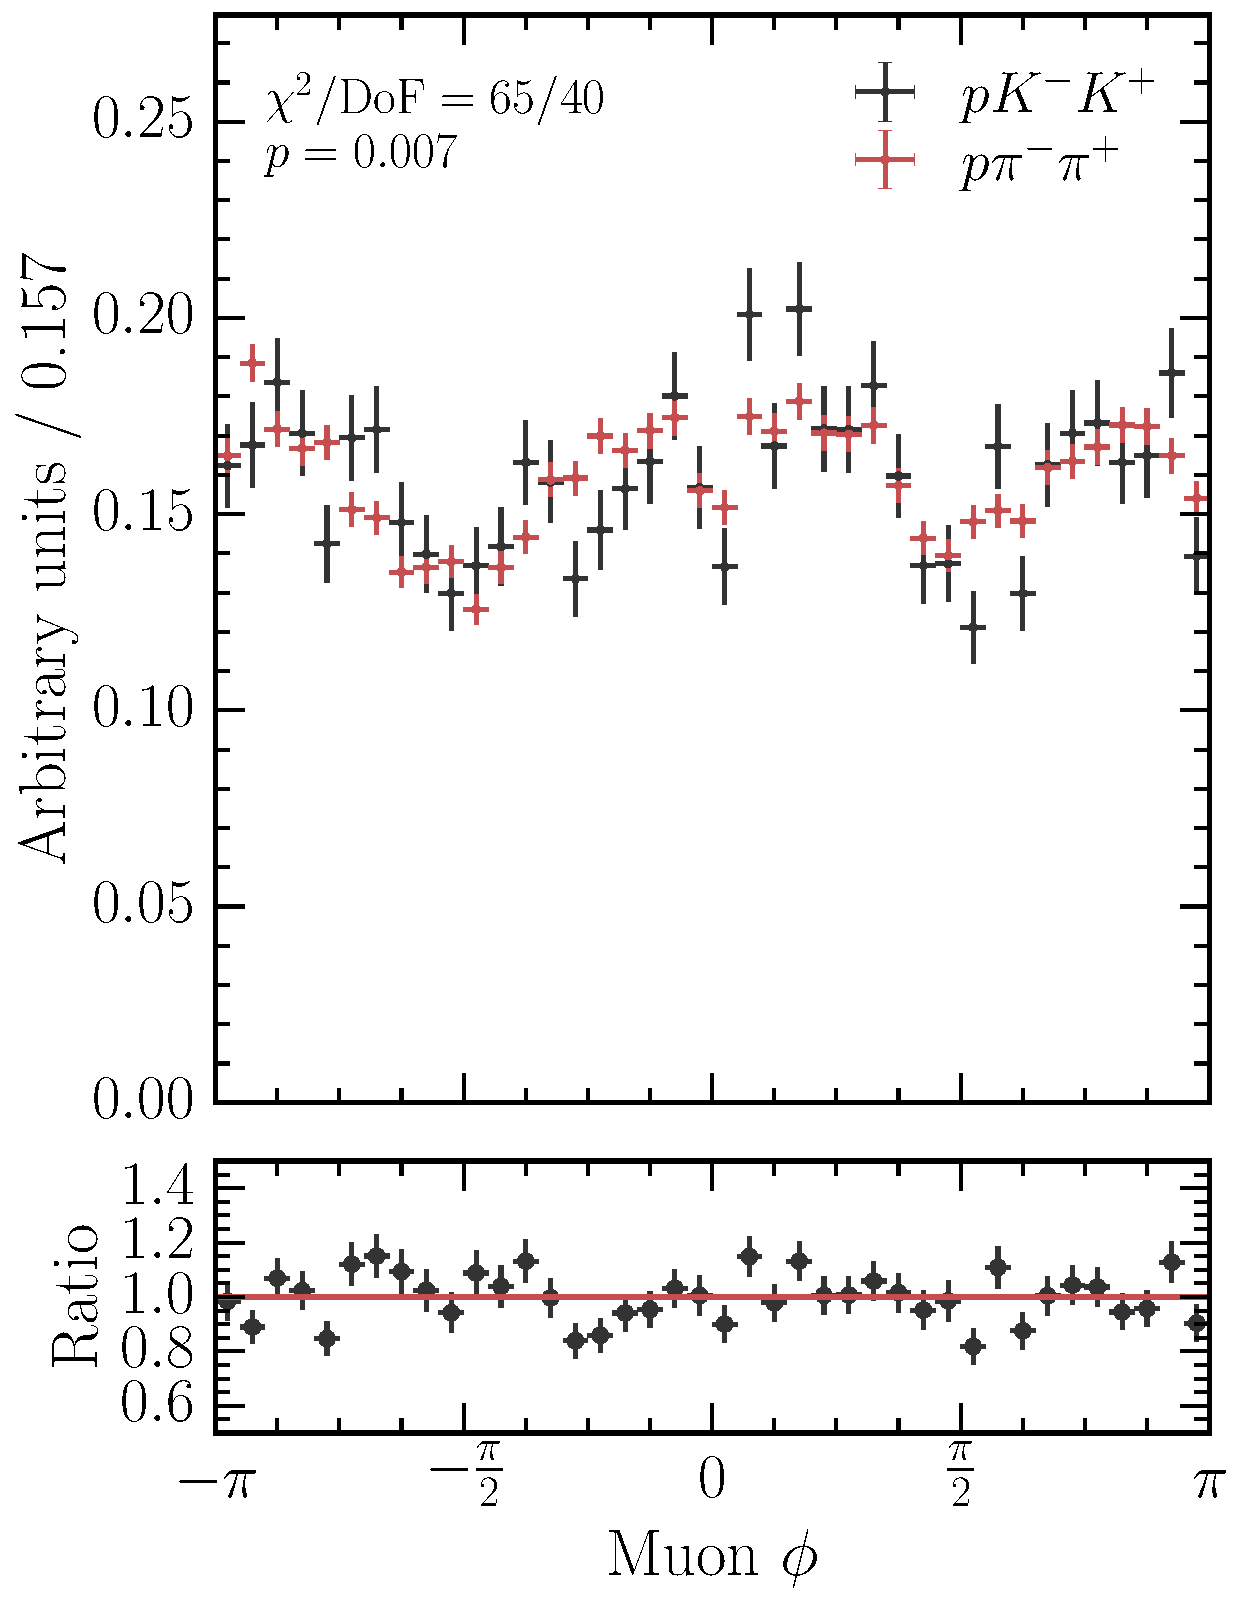
\includegraphics[width=\textwidth]{cpv/kinematic_weighting/postweighting_kinematics/LcToppipi_2012_MagDown_Lb_mu_PHI-weighted}
    \label{fig:cpv:kinematic_weighting:post:Lb_mu:PHI}
  \end{subfigure}
  \caption{%
    Clockwise from the top left: total momentum, transverse momentum, angle 
    $\phi$, and pseudorapidity of the muon from the \PLambdab, weighted by the 
    product of signal sWeights and kinematic weights.
    The 2012 magnet down data is shown.
  }
  \label{fig:cpv:kinematic_weighting:post:Lb_mu}
\end{figure}

\begin{figure}
  \begin{subfigure}[b]{0.4\textwidth}
    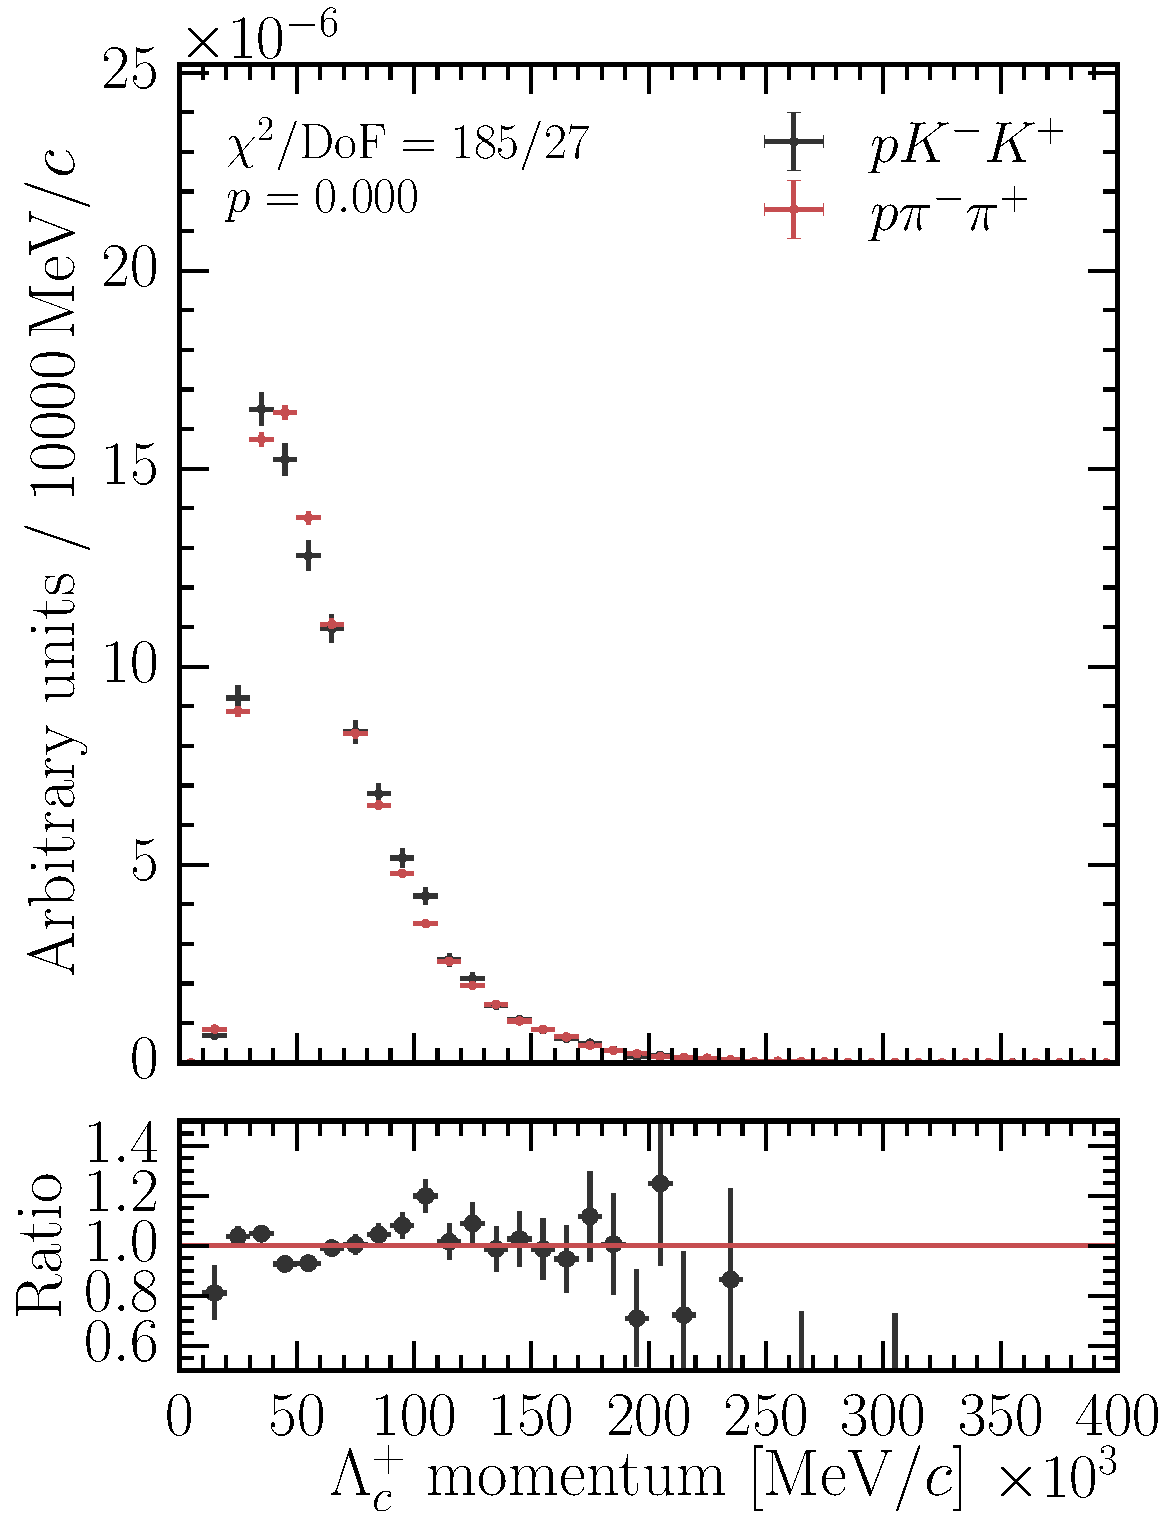
\includegraphics[width=\textwidth]{cpv/kinematic_weighting/postweighting_kinematics/LcToppipi_2012_MagDown_Lc_P-weighted}
    \label{fig:cpv:kinematic_weighting:post:Lc:P}
  \end{subfigure}
  \begin{subfigure}[b]{0.4\textwidth}
    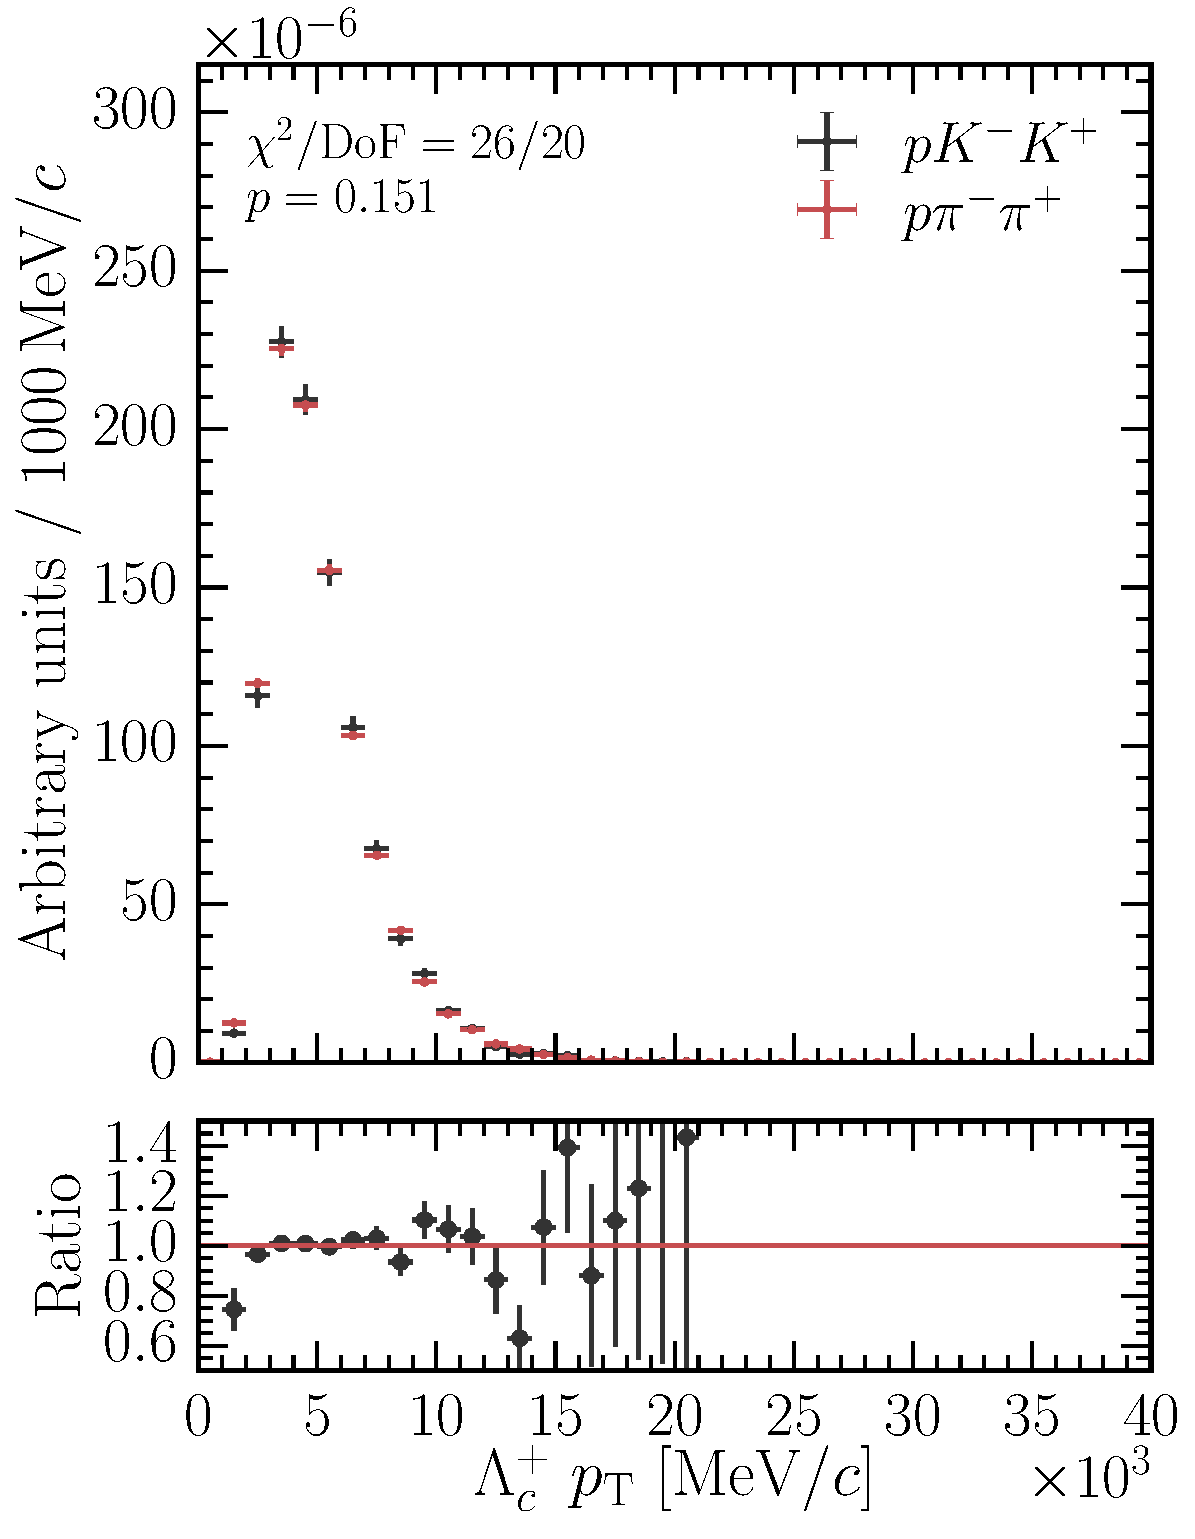
\includegraphics[width=\textwidth]{cpv/kinematic_weighting/postweighting_kinematics/LcToppipi_2012_MagDown_Lc_PT-weighted}
    \label{fig:cpv:kinematic_weighting:post:Lc:PT}
  \end{subfigure}\\
  \begin{subfigure}[b]{0.4\textwidth}
    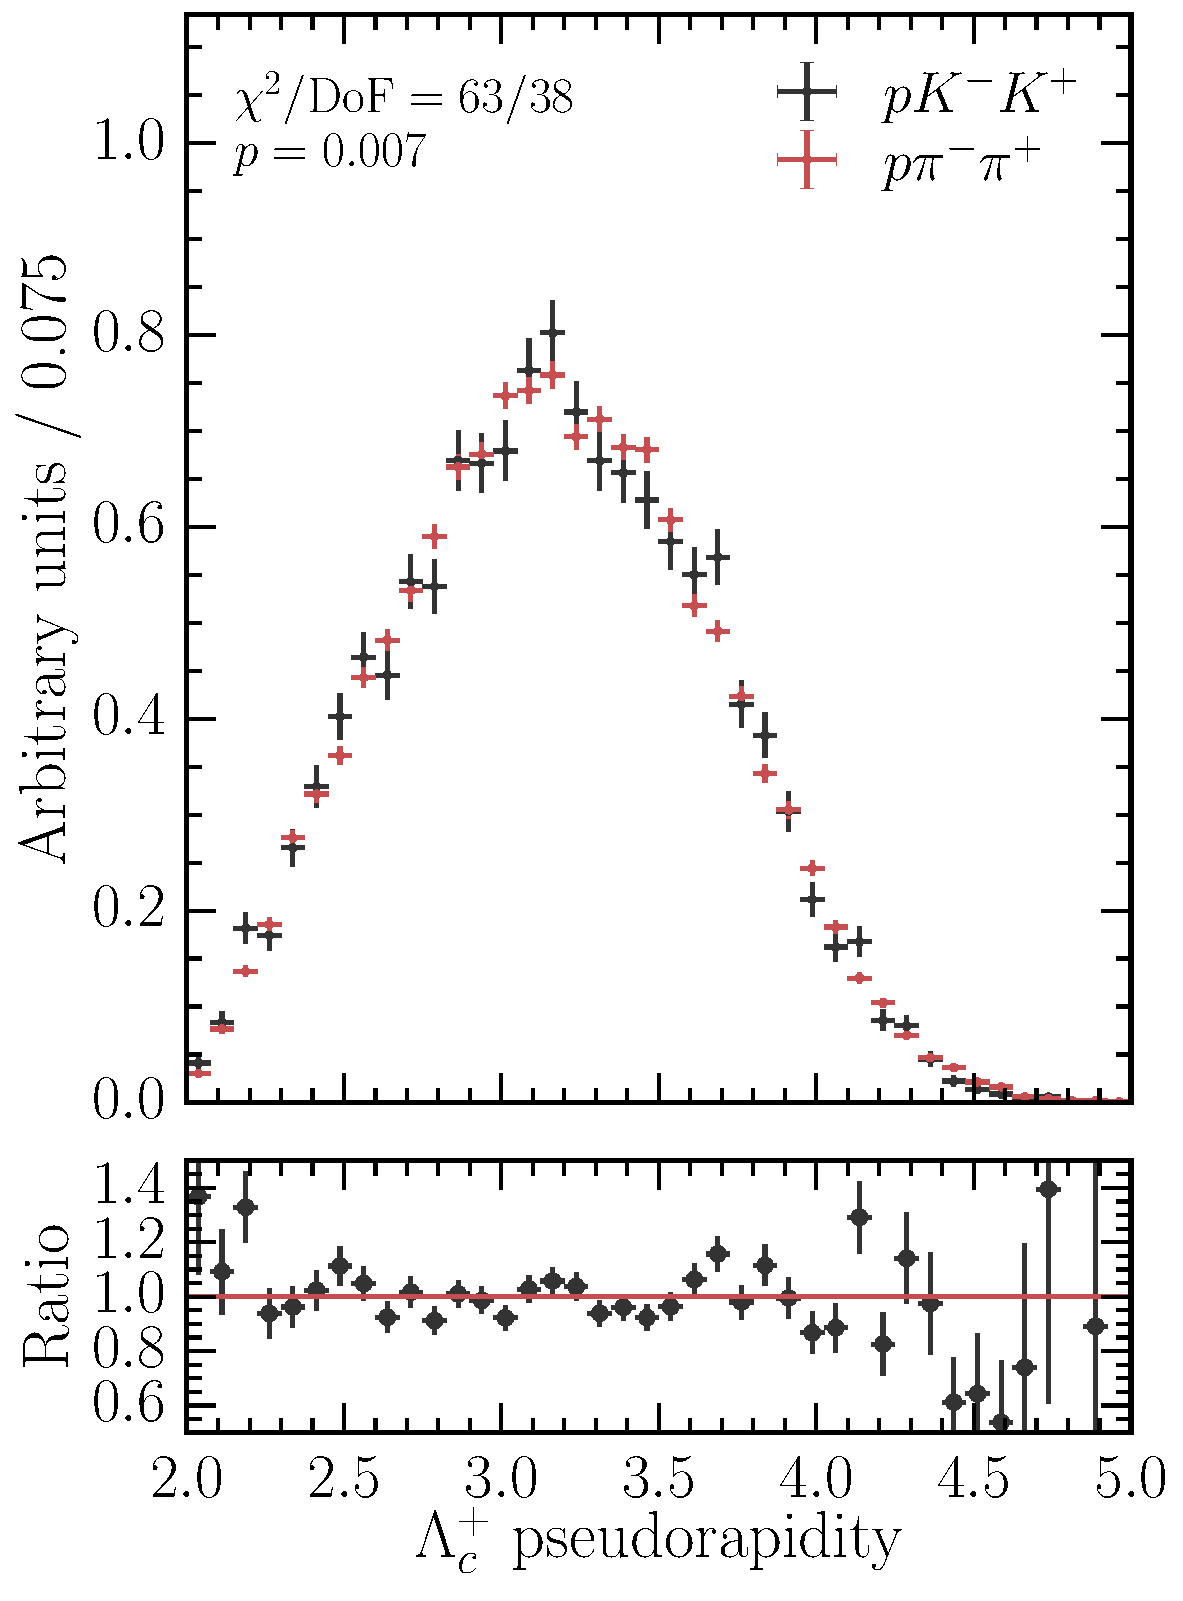
\includegraphics[width=\textwidth]{cpv/kinematic_weighting/postweighting_kinematics/LcToppipi_2012_MagDown_Lc_ETA-weighted}
    \label{fig:cpv:kinematic_weighting:post:Lc:ETA}
  \end{subfigure}
  \begin{subfigure}[b]{0.4\textwidth}
    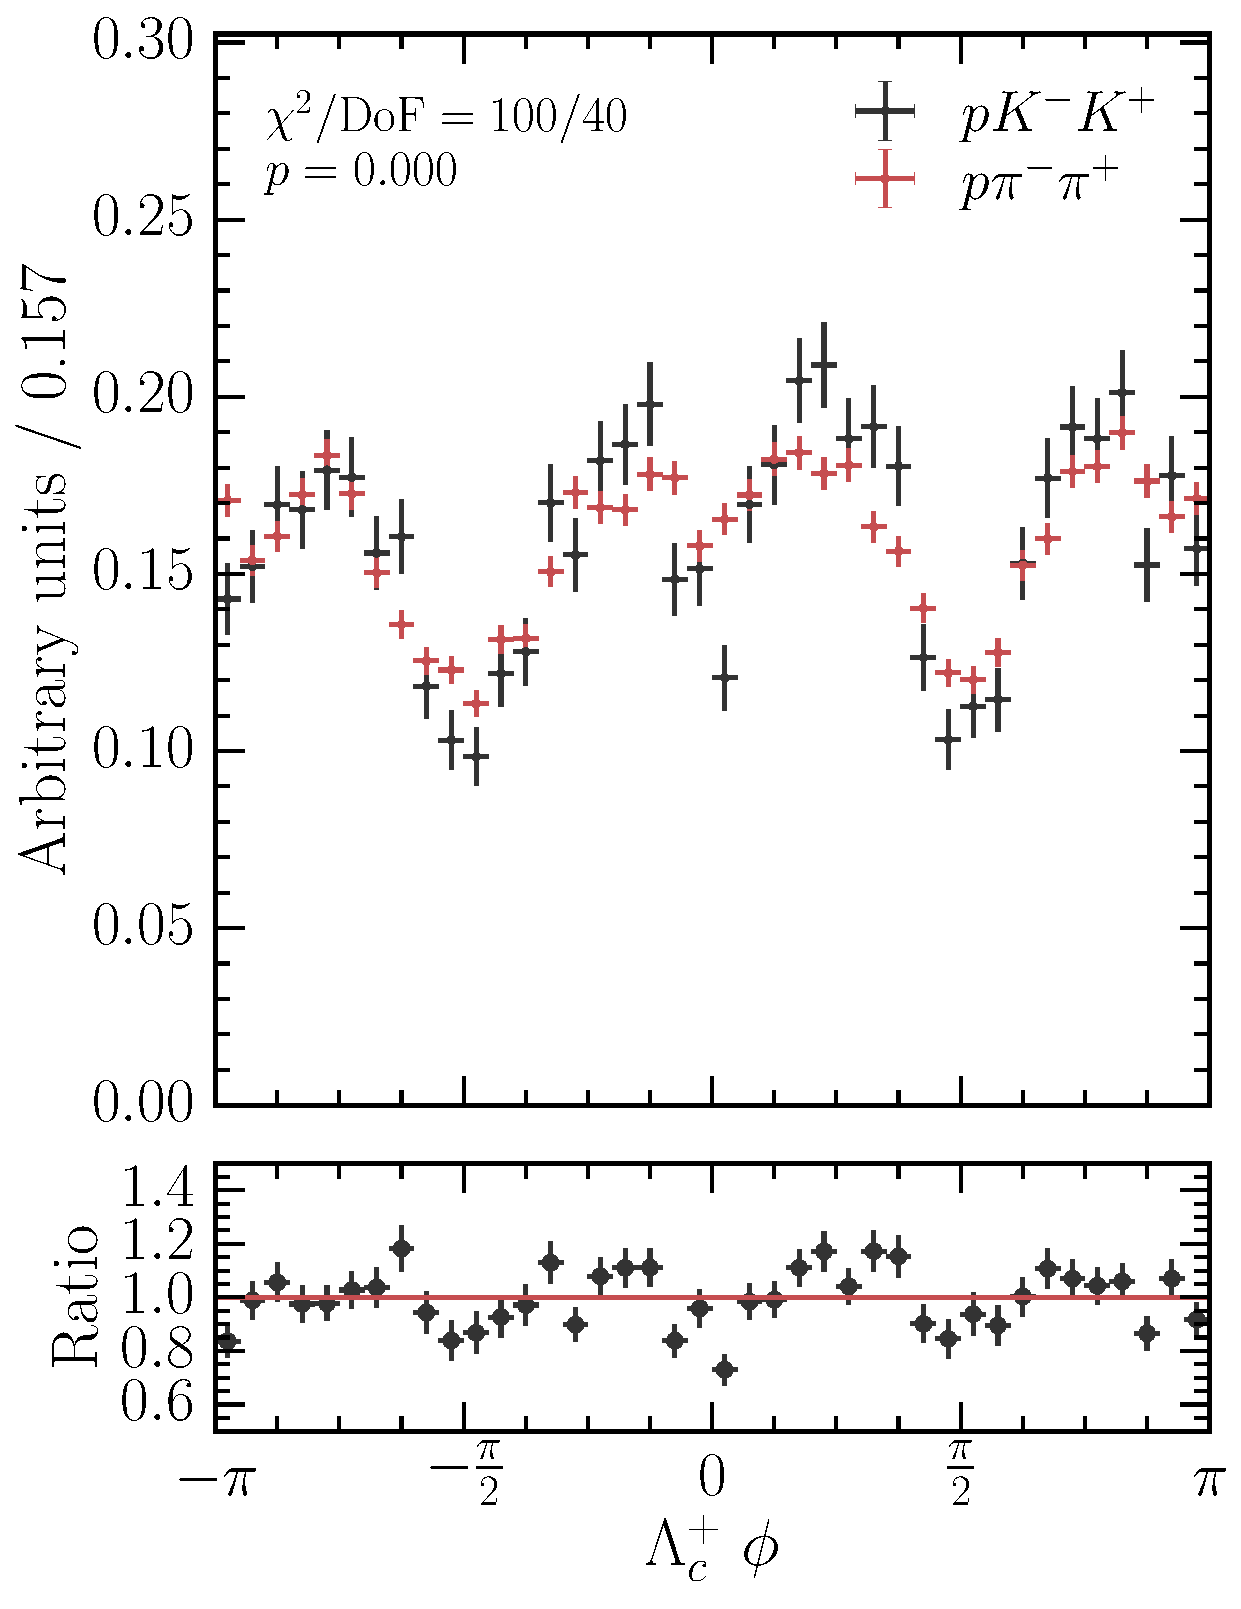
\includegraphics[width=\textwidth]{cpv/kinematic_weighting/postweighting_kinematics/LcToppipi_2012_MagDown_Lc_PHI-weighted}
    \label{fig:cpv:kinematic_weighting:post:Lc:PHI}
  \end{subfigure}
  \caption{%
    Clockwise from the top left: total momentum, transverse momentum, angle 
    $\phi$, and pseudorapidity of the \PLambdac, weighted by the product of 
    signal sWeights and kinematic weights.
    The 2012 magnet down data is shown.
  }
  \label{fig:cpv:kinematic_weighting:post:Lc}
\end{figure}

\begin{figure}
  \begin{subfigure}[b]{0.4\textwidth}
    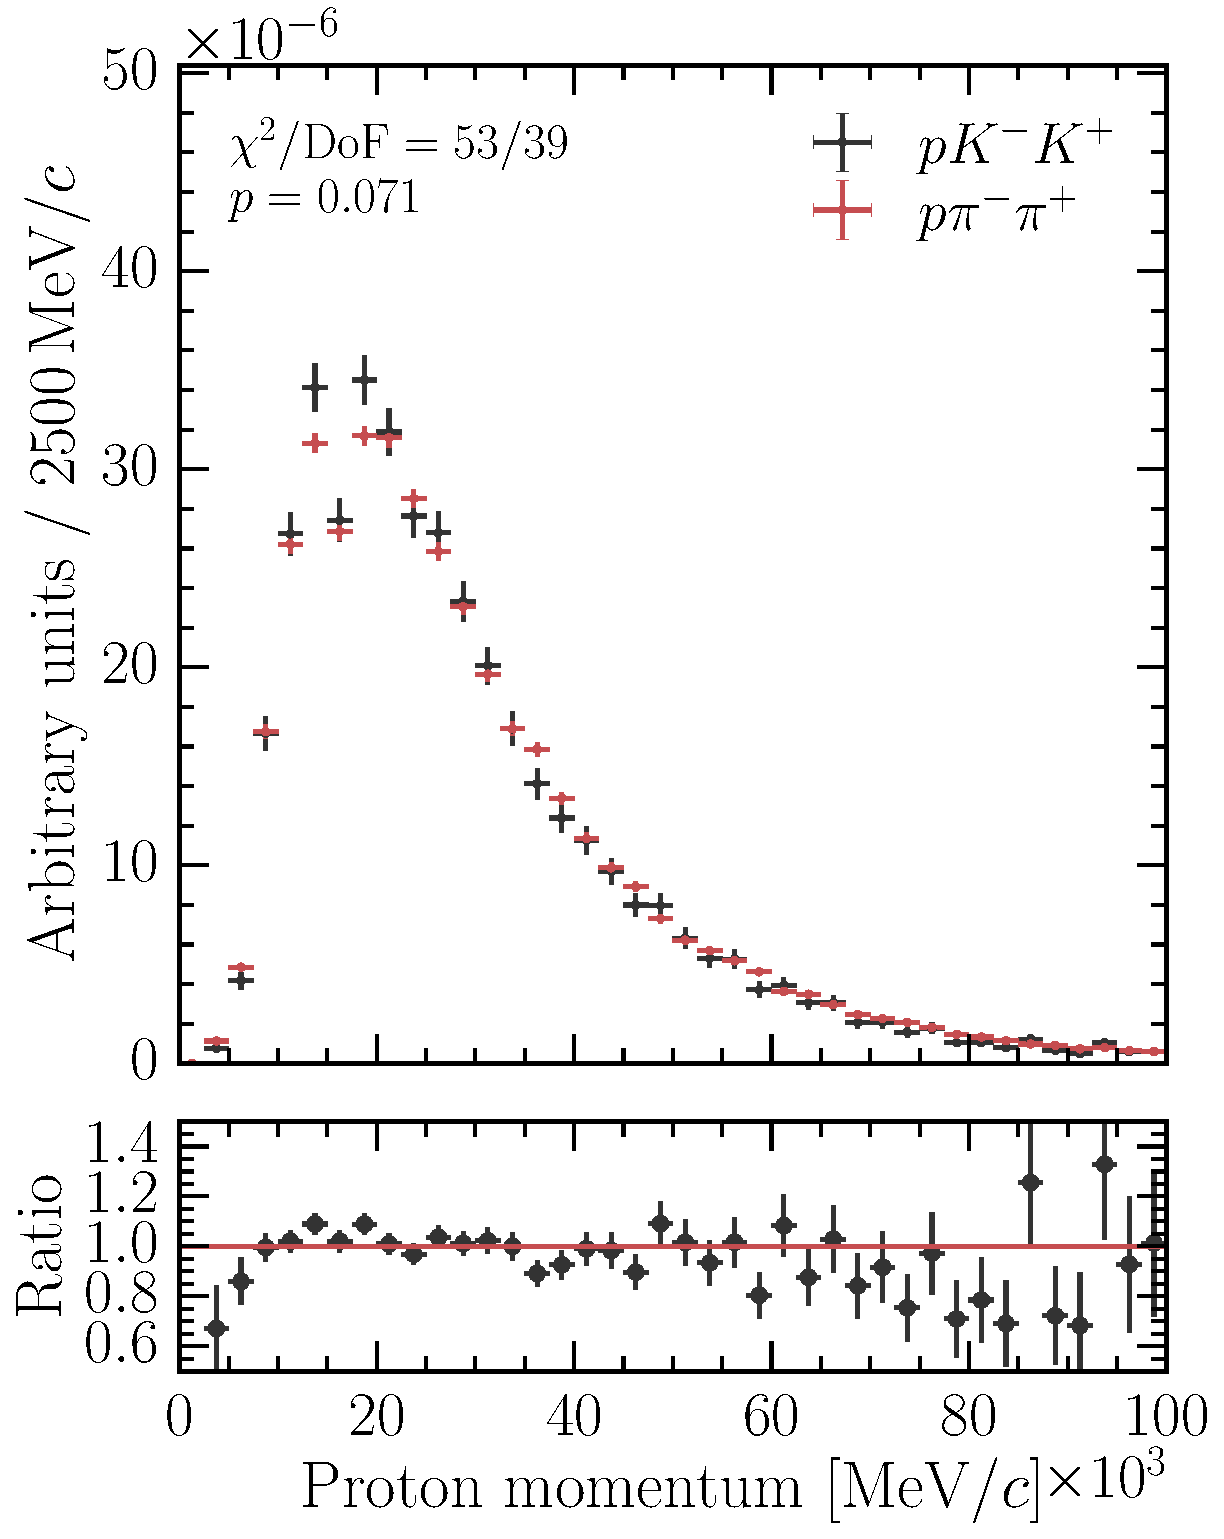
\includegraphics[width=\textwidth]{cpv/kinematic_weighting/postweighting_kinematics/LcToppipi_2012_MagDown_Lc_p_P-weighted}
    \label{fig:cpv:kinematic_weighting:post:Lc_p:P}
  \end{subfigure}
  \begin{subfigure}[b]{0.4\textwidth}
    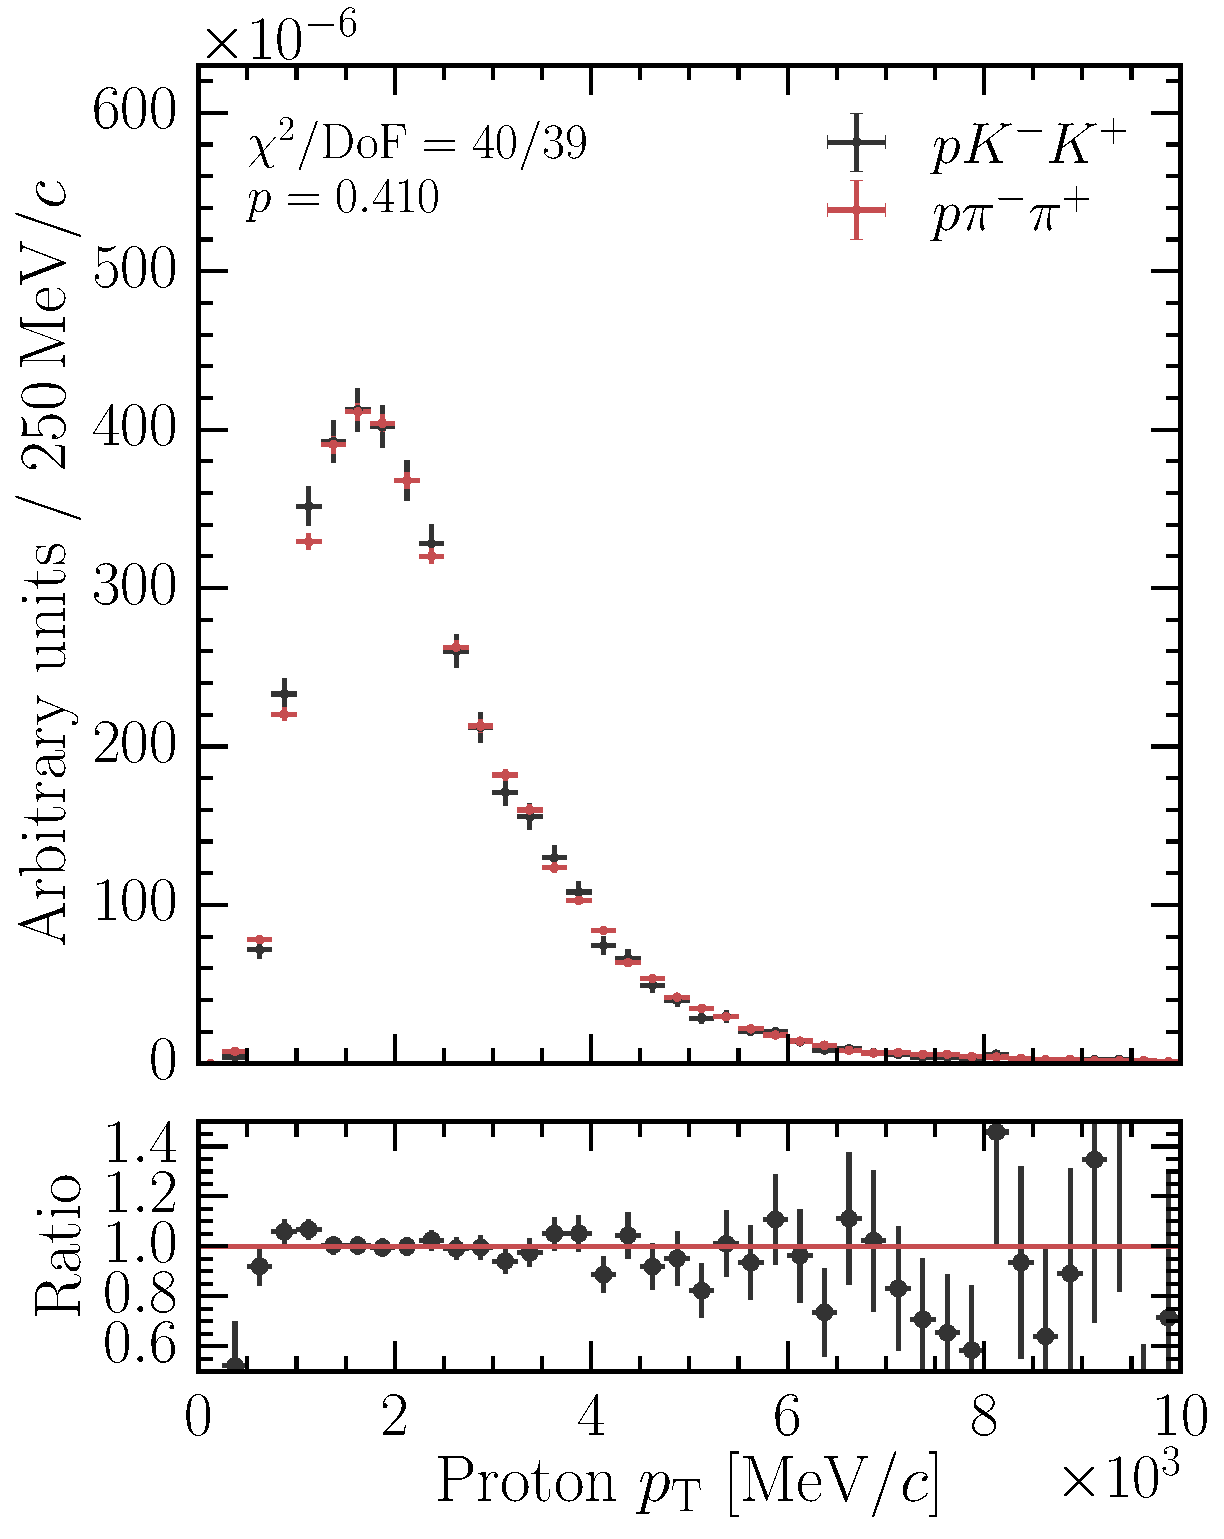
\includegraphics[width=\textwidth]{cpv/kinematic_weighting/postweighting_kinematics/LcToppipi_2012_MagDown_Lc_p_PT-weighted}
    \label{fig:cpv:kinematic_weighting:post:Lc_p:PT}
  \end{subfigure}\\
  \begin{subfigure}[b]{0.4\textwidth}
    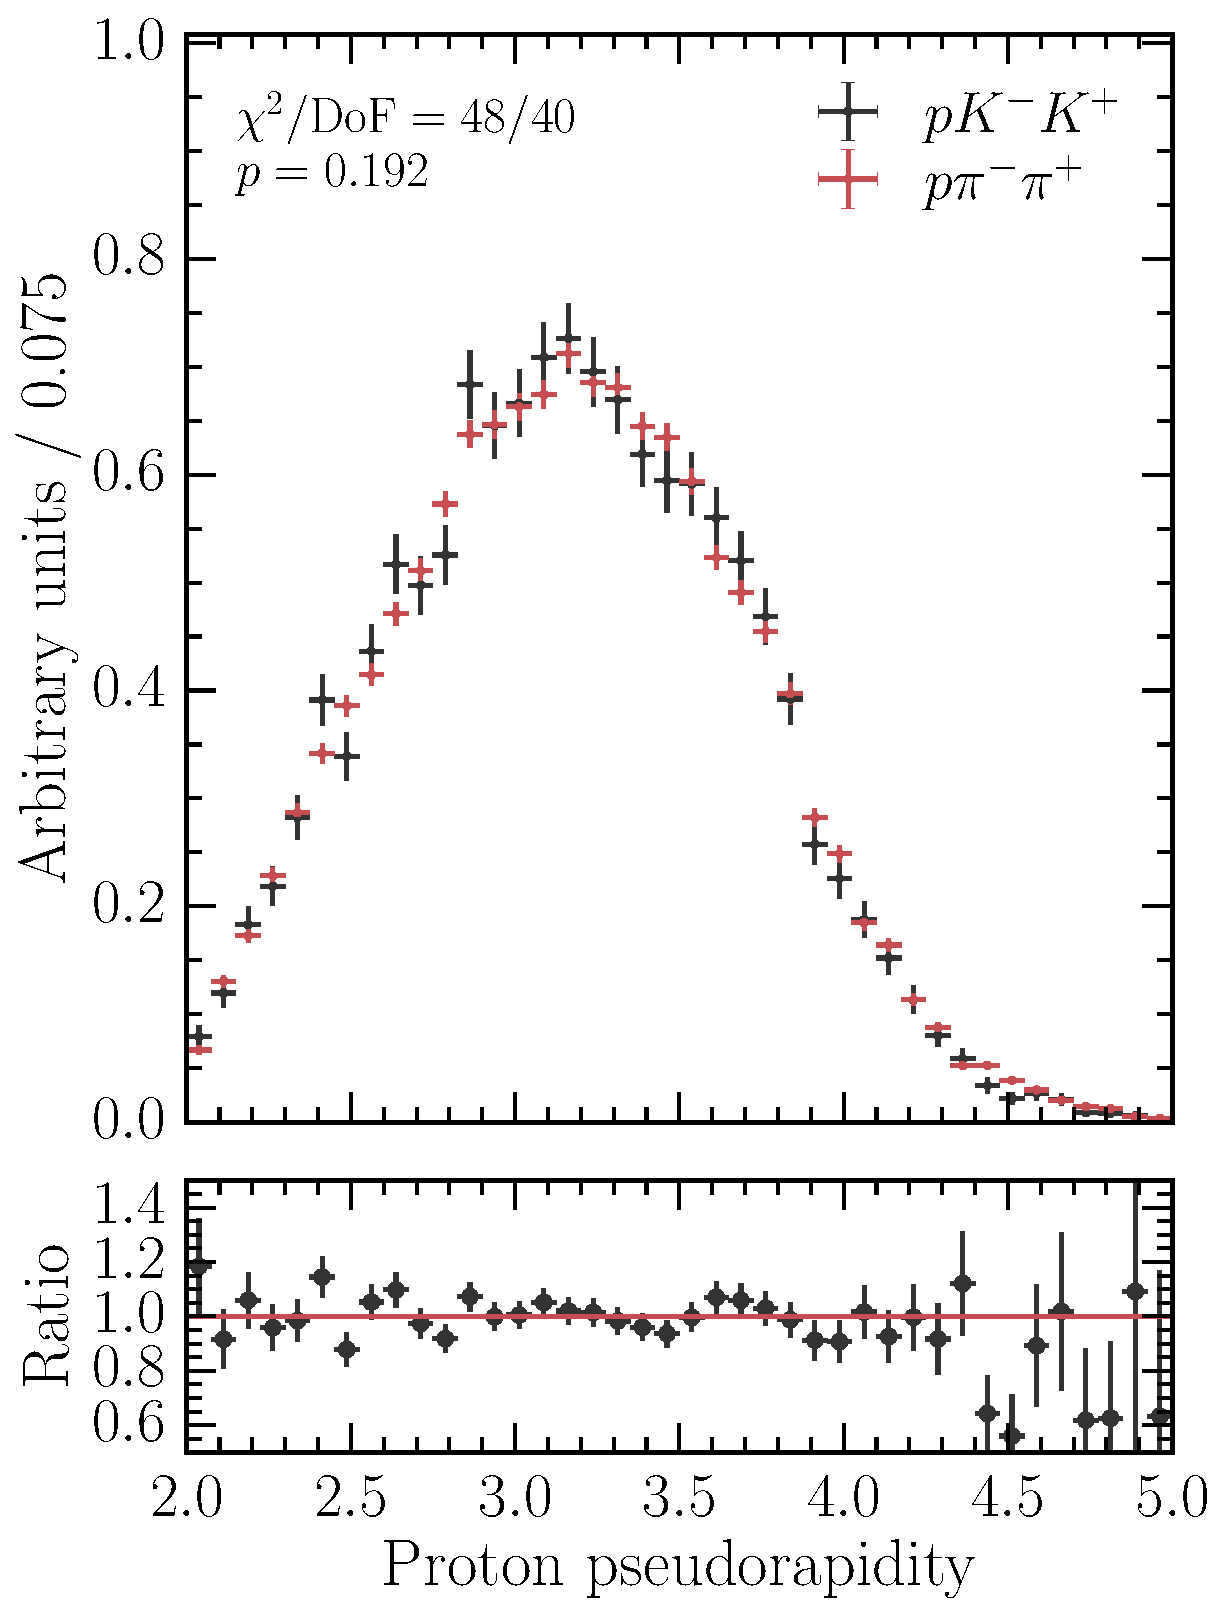
\includegraphics[width=\textwidth]{cpv/kinematic_weighting/postweighting_kinematics/LcToppipi_2012_MagDown_Lc_p_ETA-weighted}
    \label{fig:cpv:kinematic_weighting:post:Lc_p:ETA}
  \end{subfigure}
  \begin{subfigure}[b]{0.4\textwidth}
    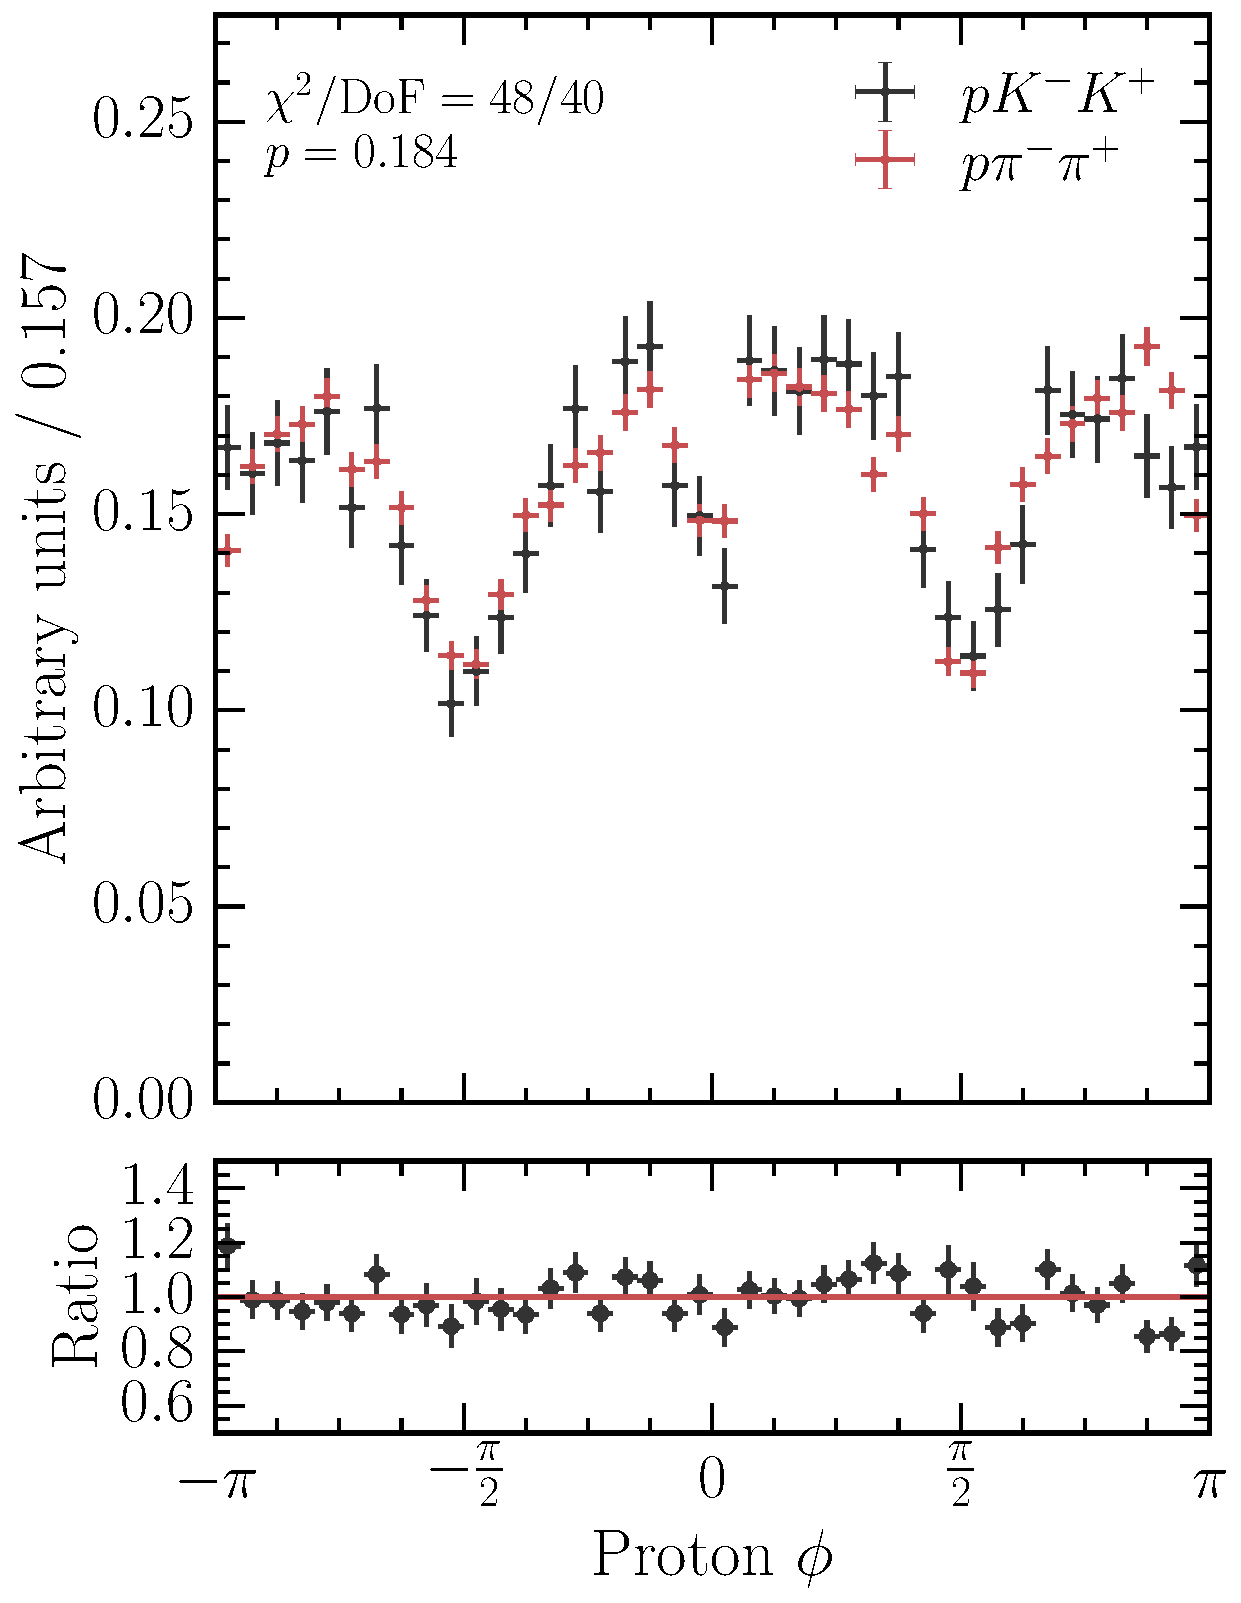
\includegraphics[width=\textwidth]{cpv/kinematic_weighting/postweighting_kinematics/LcToppipi_2012_MagDown_Lc_p_PHI-weighted}
    \label{fig:cpv:kinematic_weighting:post:Lc_p:PHI}
  \end{subfigure}
  \caption{%
    Clockwise from the top left: total momentum, transverse momentum, angle 
    $\phi$, and pseudorapidity of the proton from the \PLambdac, weighted by 
    the product of signal sWeights and kinematic weights.
    The 2012 magnet down data is shown.
  }
  \label{fig:cpv:kinematic_weighting:post:Lc_p}
\end{figure}

\begin{figure}
  \begin{subfigure}[b]{0.5\textwidth}
    \centering
    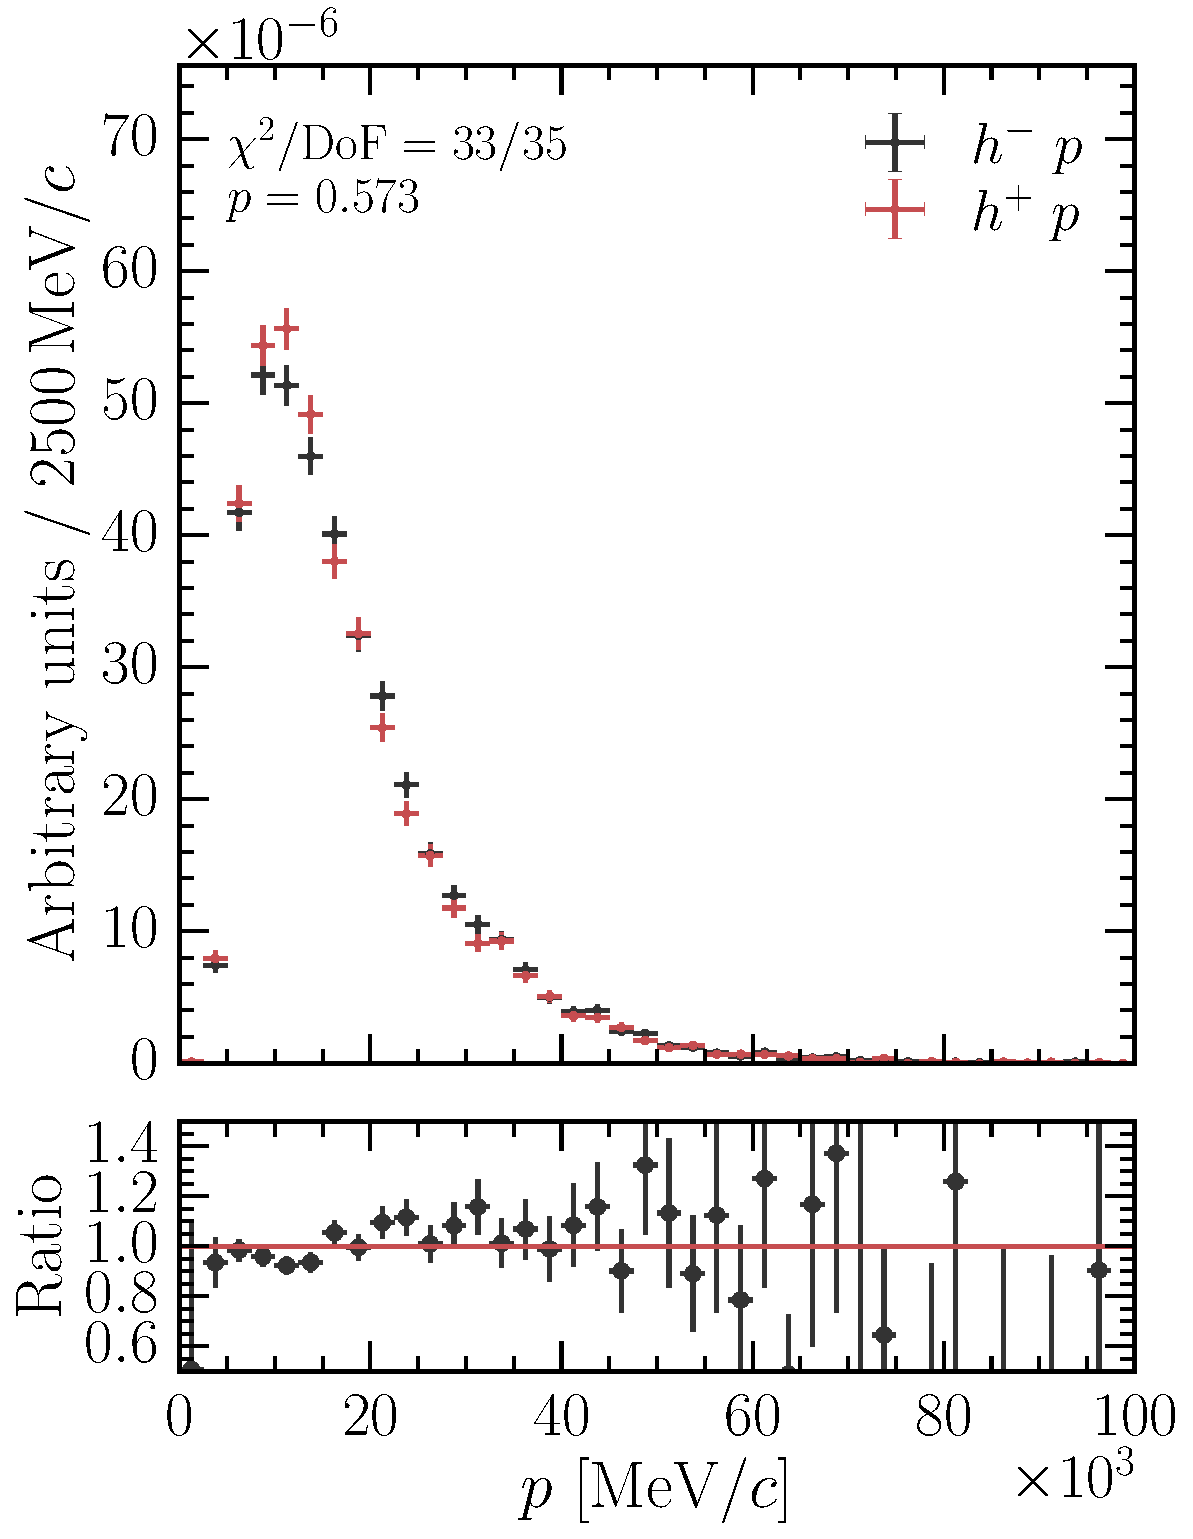
\includegraphics[width=0.8\textwidth]{cpv/kinematic_weighting/postweighting_kinematics/LcToppipi_2012_MagDown_h1_h2_P_LcTopKK-weighted}
    \label{fig:cpv:kinematic_weighting:post:pKK_h1h2:P}
  \end{subfigure}
  \begin{subfigure}[b]{0.5\textwidth}
    \centering
    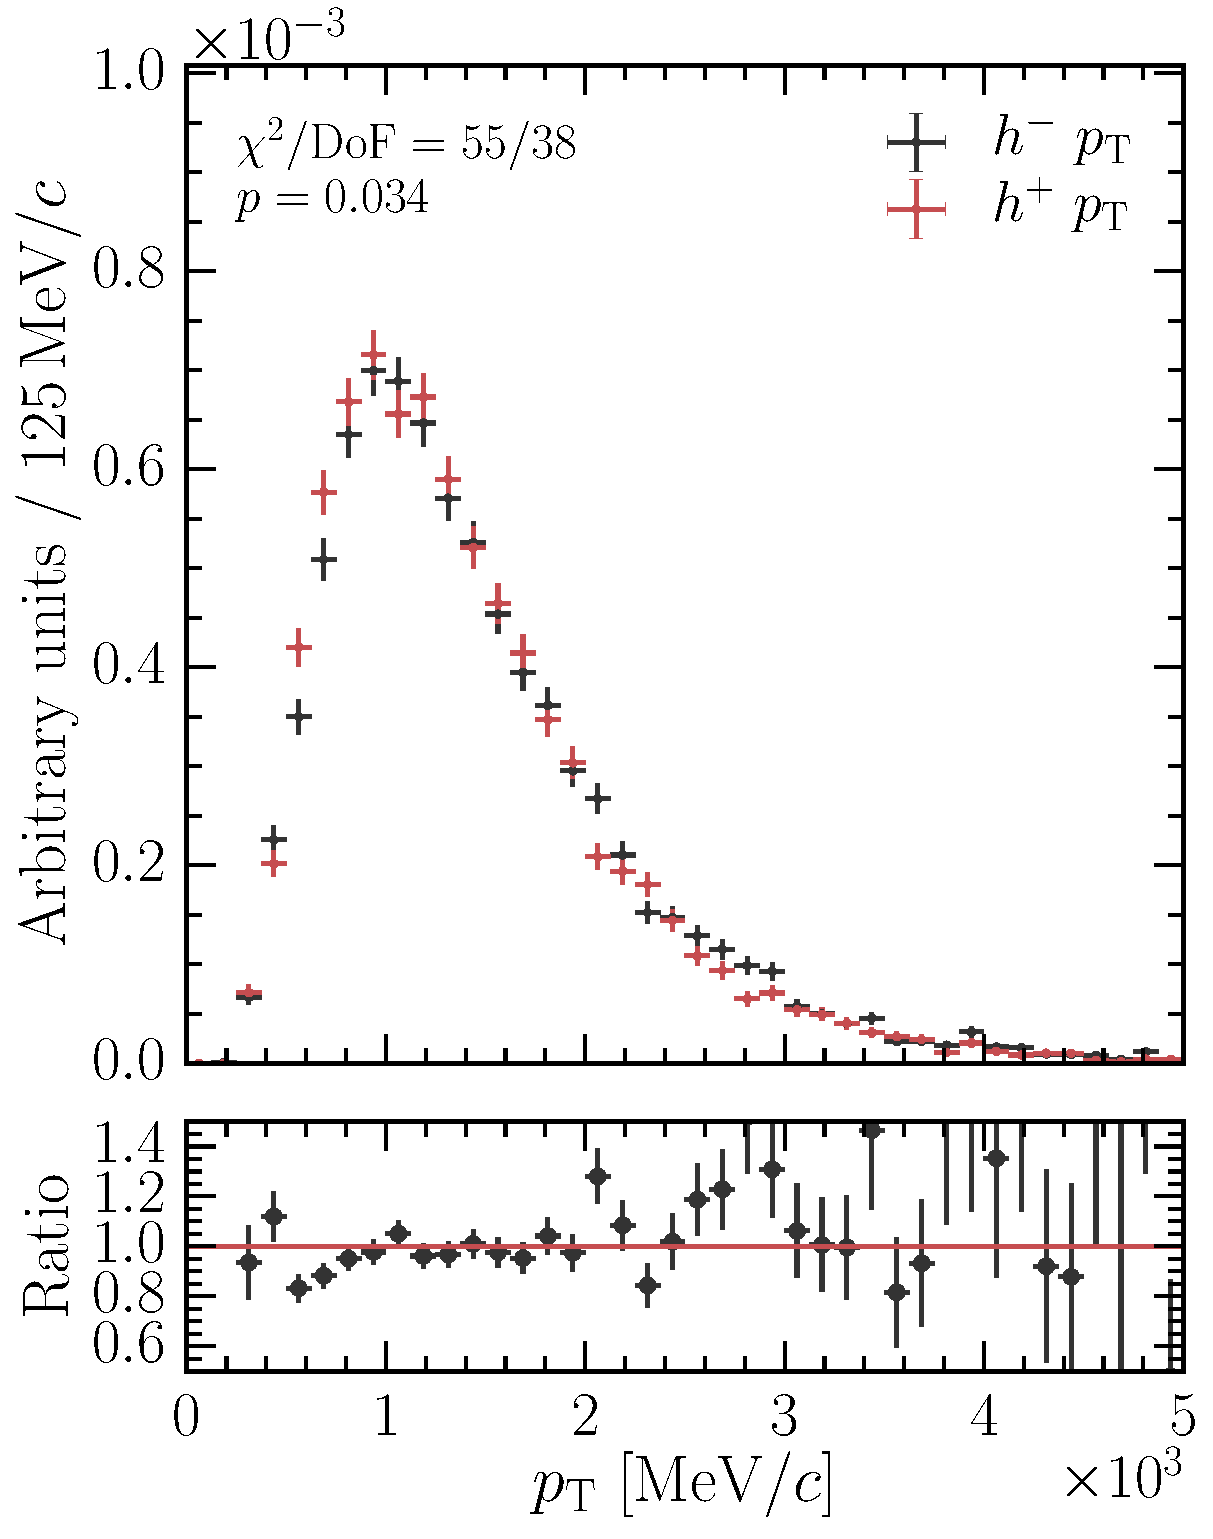
\includegraphics[width=0.8\textwidth]{cpv/kinematic_weighting/postweighting_kinematics/LcToppipi_2012_MagDown_h1_h2_PT_LcTopKK-weighted}
    \label{fig:cpv:kinematic_weighting:post:pKK_h1h2:PT}
  \end{subfigure}\\
  \begin{subfigure}[b]{\textwidth}
    \centering
    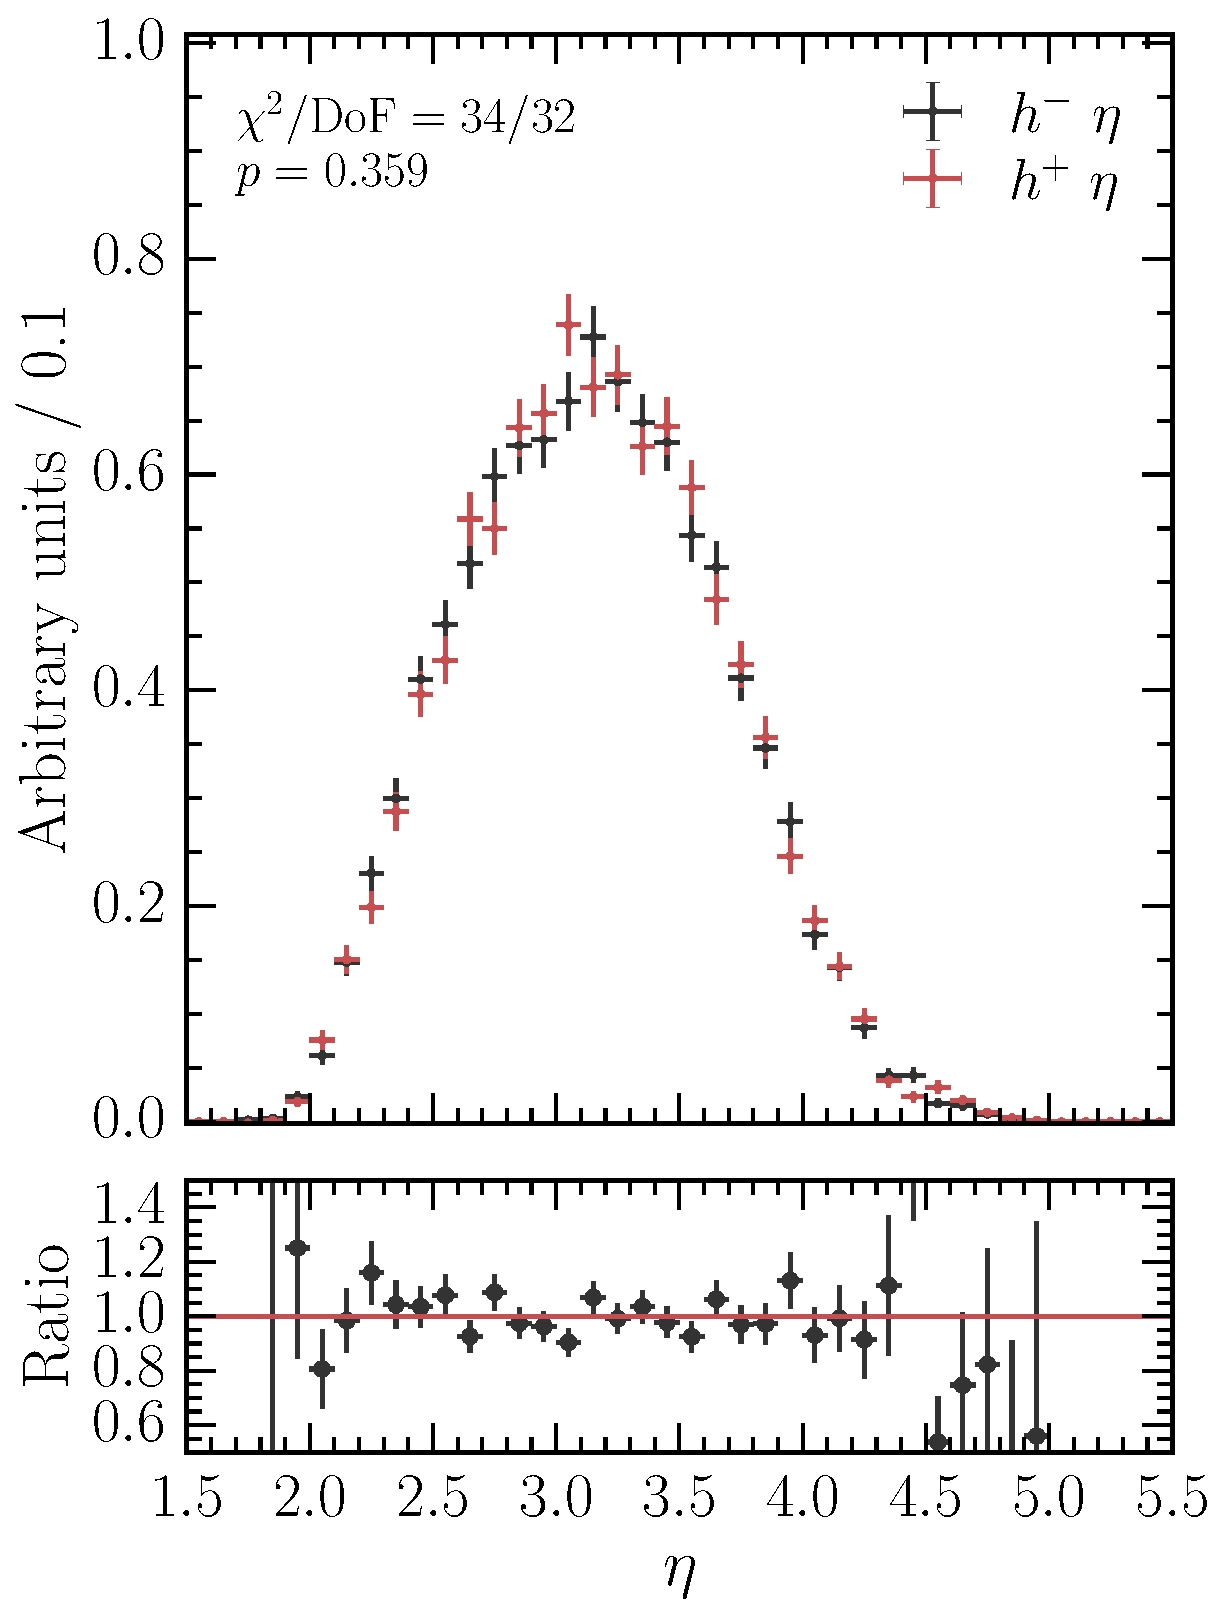
\includegraphics[width=0.4\textwidth]{cpv/kinematic_weighting/postweighting_kinematics/LcToppipi_2012_MagDown_h1_h2_ETA_LcTopKK-weighted}
    \label{fig:cpv:kinematic_weighting:post:pKK_h1h2:ETA}
  \end{subfigure}
  \caption{%
    Clockwise from the top left: total momentum, transverse momentum, and 
    pseudorapidity of the \PKminus\ and \PKplus\ \PLambdac\ children in the 
    \pKK\ data, weighted by the product of signal sWeights and kinematic 
    weights.
    The 2012 magnet down data is shown.
  }
  \label{fig:cpv:kinematic_weighting:post:pKK_h1h2}
\end{figure}

\begin{figure}
  \begin{subfigure}[b]{0.5\textwidth}
    \centering
    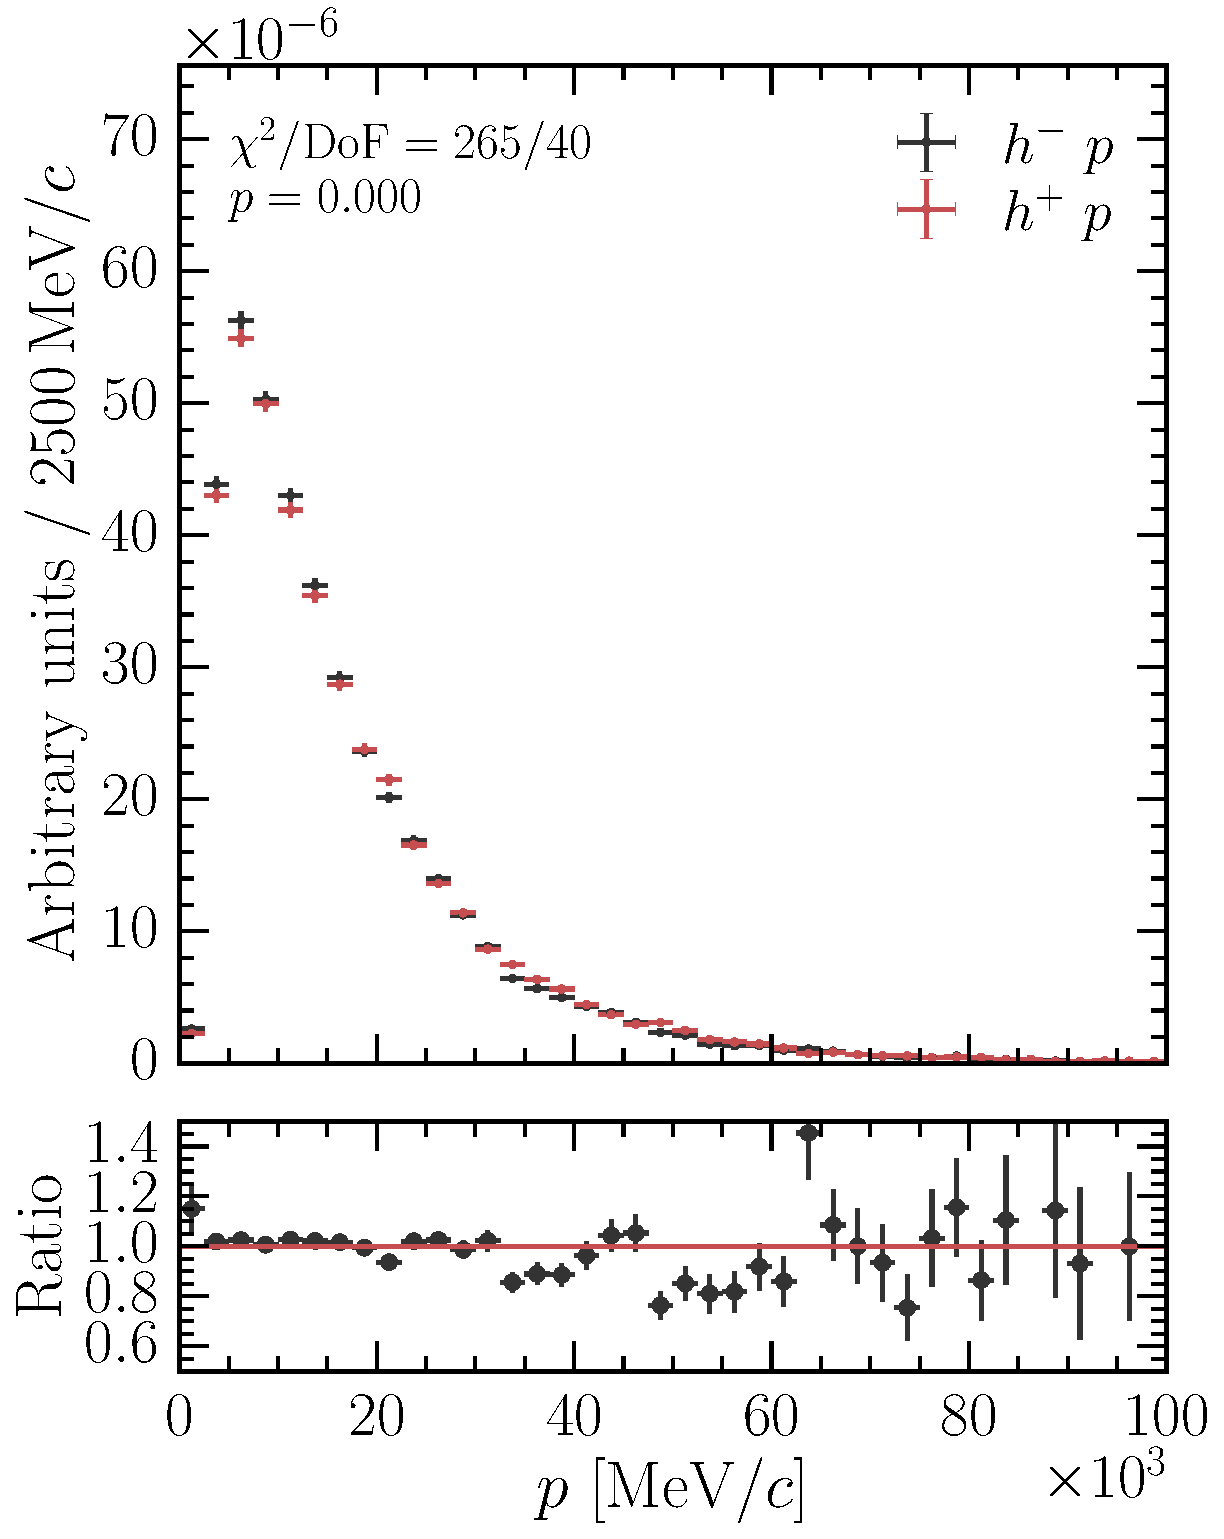
\includegraphics[width=0.8\textwidth]{cpv/kinematic_weighting/postweighting_kinematics/LcToppipi_2012_MagDown_h1_h2_P_LcToppipi-weighted}
    \label{fig:cpv:kinematic_weighting:post:ppipi_h1h2:P}
  \end{subfigure}
  \begin{subfigure}[b]{0.5\textwidth}
    \centering
    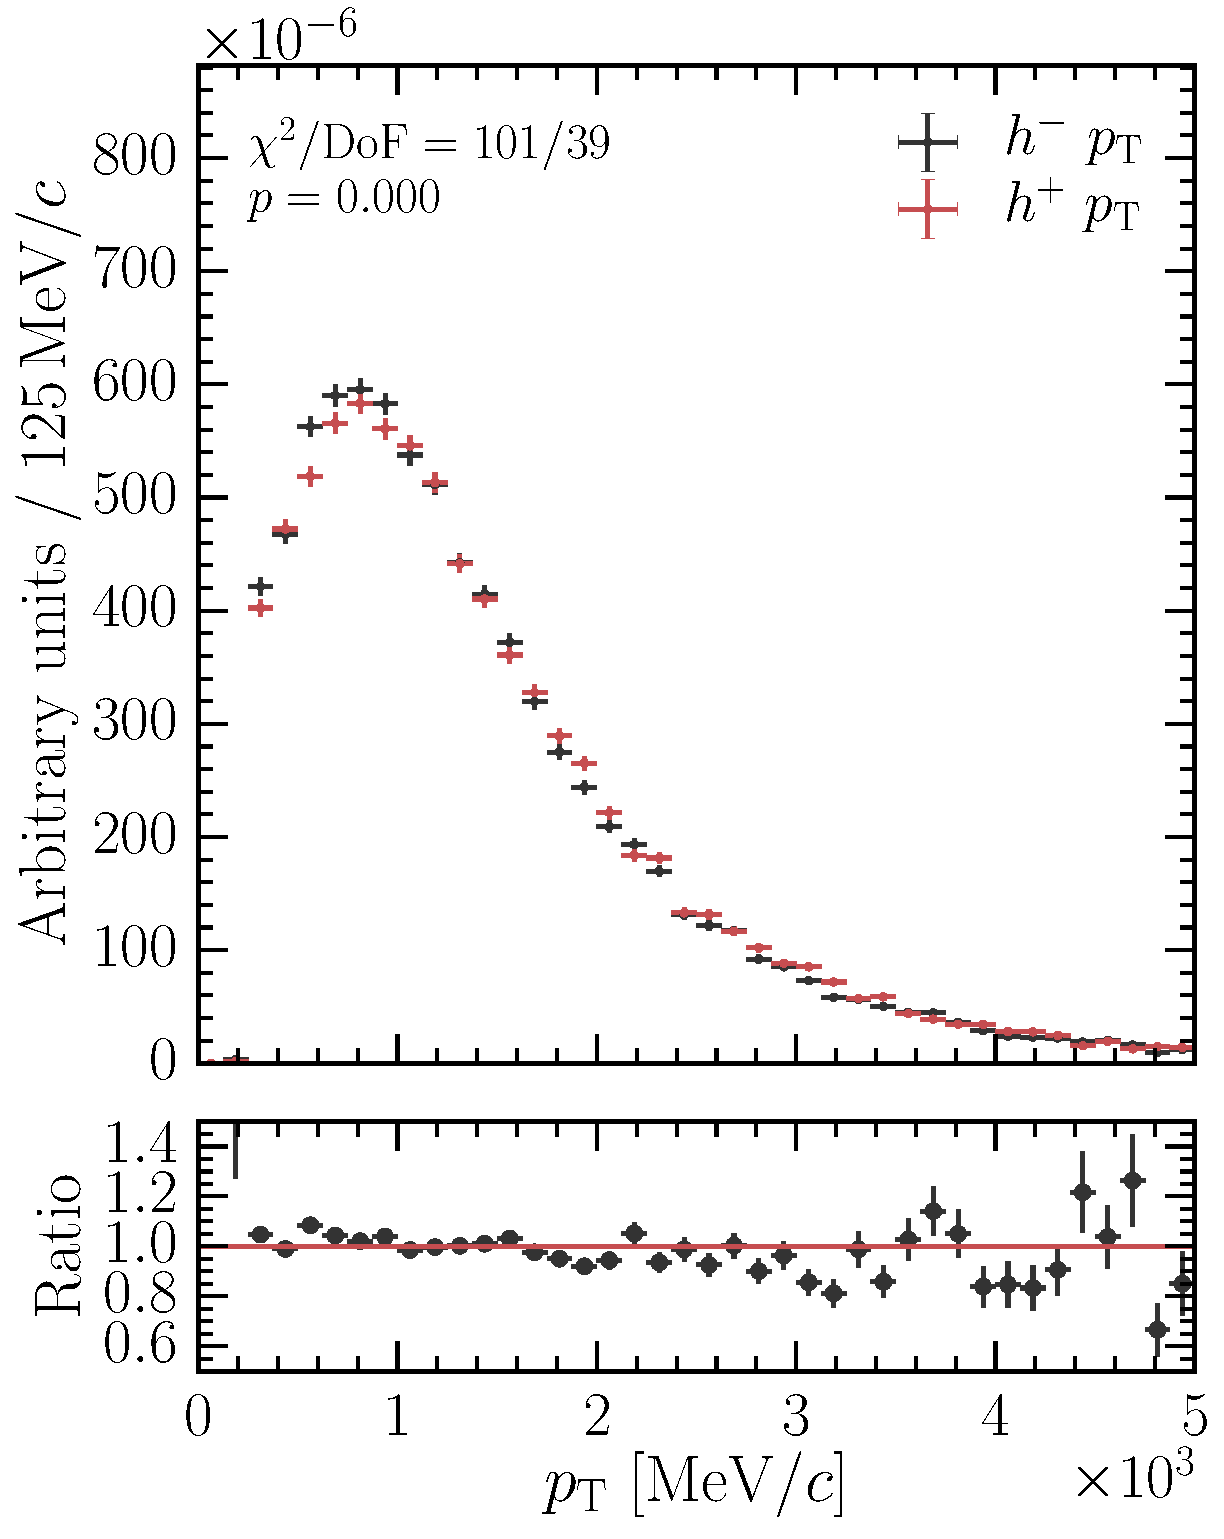
\includegraphics[width=0.8\textwidth]{cpv/kinematic_weighting/postweighting_kinematics/LcToppipi_2012_MagDown_h1_h2_PT_LcToppipi-weighted}
    \label{fig:cpv:kinematic_weighting:post:ppipi_h1h2:PT}
  \end{subfigure}\\
  \begin{subfigure}[b]{\textwidth}
    \centering
    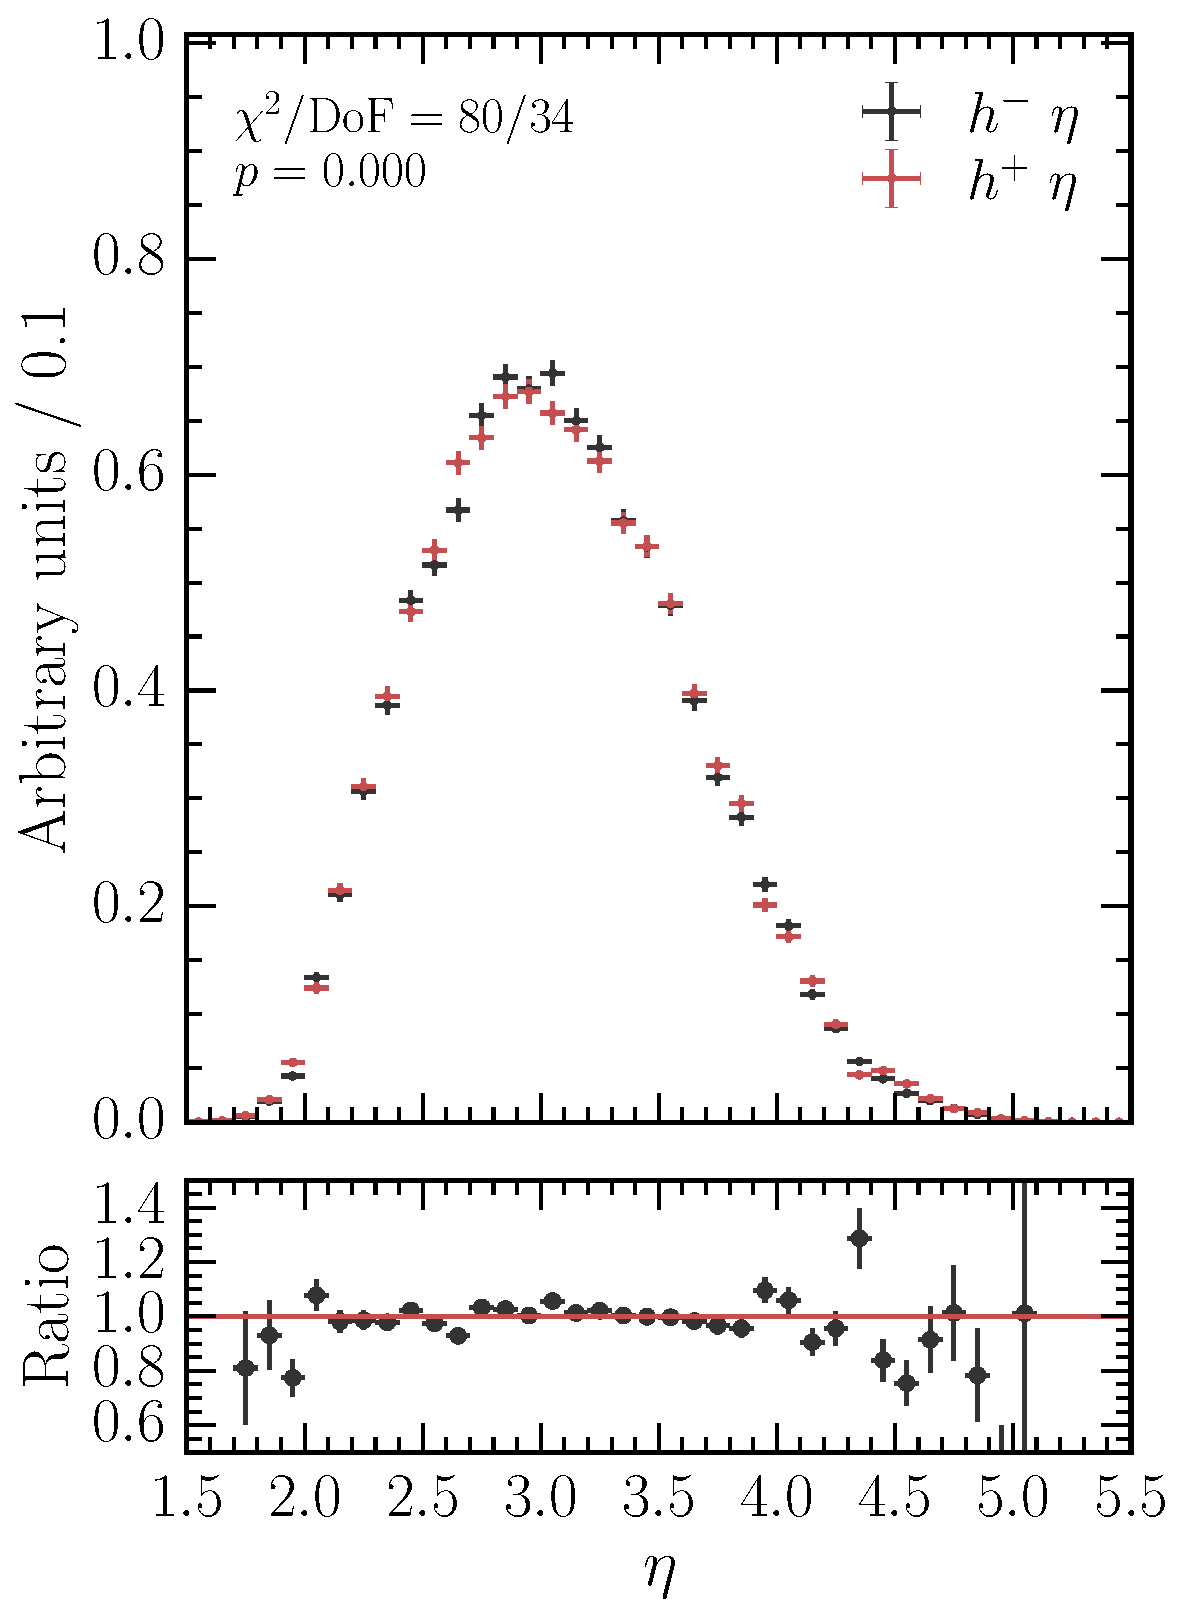
\includegraphics[width=0.4\textwidth]{cpv/kinematic_weighting/postweighting_kinematics/LcToppipi_2012_MagDown_h1_h2_ETA_LcToppipi-weighted}
    \label{fig:cpv:kinematic_weighting:post:ppipi_h1h2:ETA}
  \end{subfigure}
  \caption{%
    Clockwise from the top left: total momentum, transverse momentum, and 
    pseudorapidity of the \Ppiminus\ and \Ppiplus\ \PLambdac\ children in the 
    \ppipi\ data, weighted by the product of signal sWeights and kinematic 
    weights.
    The 2012 magnet down data is shown.
  }
  \label{fig:cpv:kinematic_weighting:post:ppipi_h1h2}
\end{figure}

\begin{figure}
  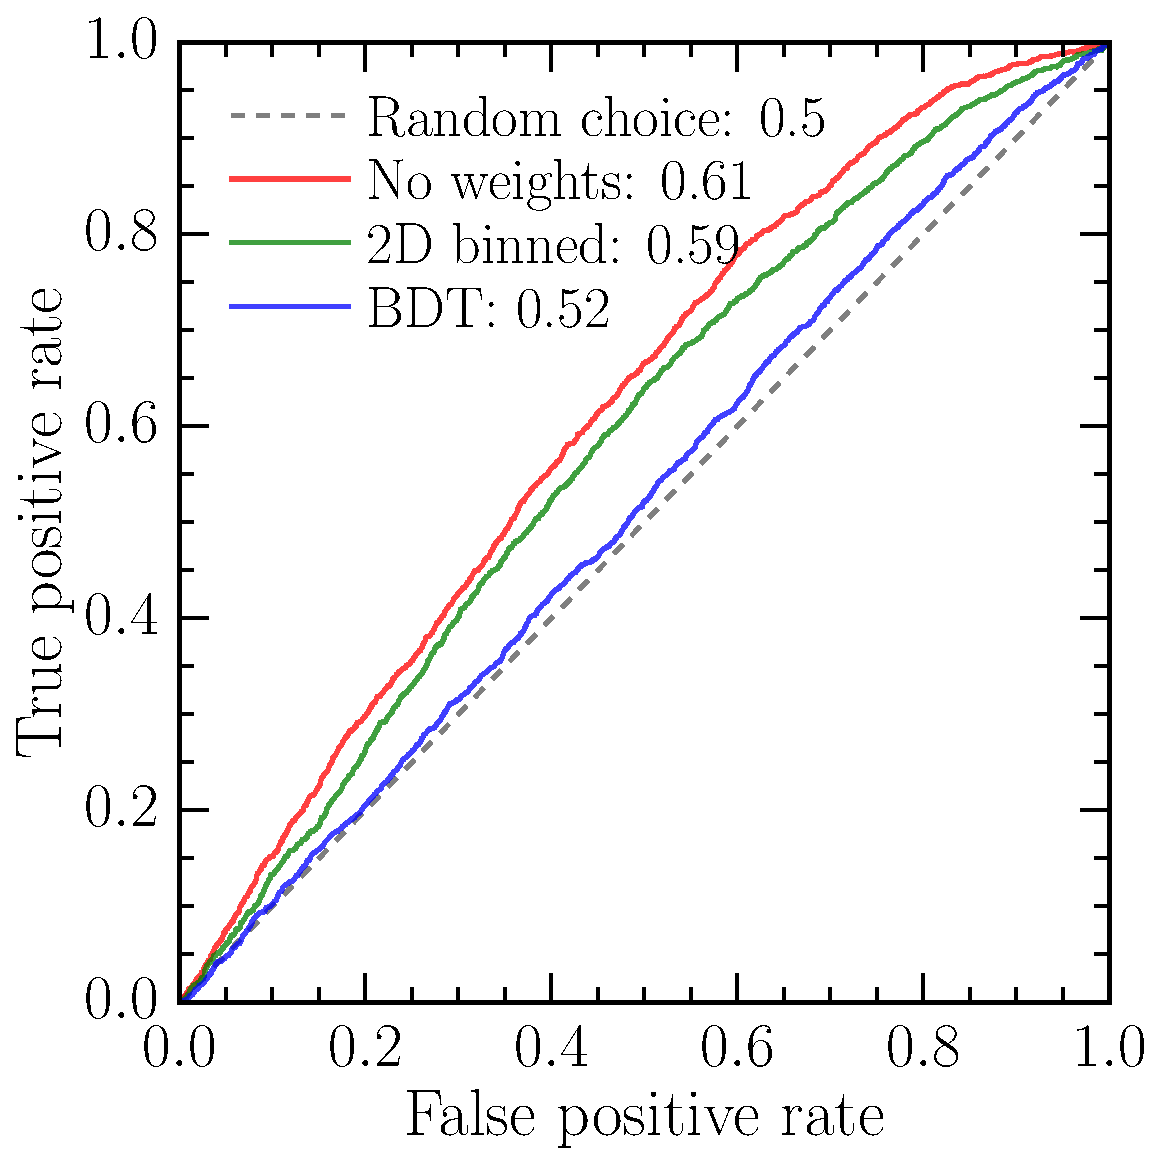
\includegraphics[width=\textwidth]{cpv/kinematic_weighting/postweighting_kinematics/LcToppipi_2012_MagDown_roc_curves}
  \caption{%
    ROC curves for different kinematic weighting techniques.
    The ``no weights'' data has no \emph{kinematic} weights applied, only 
    signal sWeights.
    The ``2D binned'' and ``\ac{BDT}'' data uses the product of the respective 
    kinematic weights and the signal sWeights for the \ppipi\ data, and uses
    signal sWeights for the \pKK\ data.
    The area under each \ac{ROC} curve, the \acs{AUC}, is given in the legend.
  }
  \label{fig:cpv:kinematic_weighting:post:roc}
\end{figure}
